\documentclass[final,12pt]{colt2018} % Anonymized submission
% \documentclass{colt2017} % Include author names

% The following packages will be automatically loaded:
% amsmath, amssymb, natbib, graphicx, url, algorithm2e


\usepackage{times}
\usepackage{physics}
\usepackage{natbib}
\usepackage{mathtools}

\newcommand{\BEAS}{\begin{eqnarray*}}
\newcommand{\EEAS}{\end{eqnarray*}}
\newcommand{\BEA}{\begin{eqnarray}}
\newcommand{\EEA}{\end{eqnarray}}
\newcommand{\BA}{\begin{align}}
\newcommand{\EA}{\end{align}}
\newcommand{\BEQ}{\begin{equation}}
\newcommand{\EEQ}{\end{equation}}
\newcommand{\BIT}{\begin{itemize}}
\newcommand{\EIT}{\end{itemize}}
\newcommand{\BNUM}{\begin{enumerate}}
\newcommand{\ENUM}{\end{enumerate}}
\newcommand{\diag}{\mathop{\rm diag}}
\newcommand{\Diag}{\mathop{\rm Diag}}


\newcommand{\x}{\mathbf{x}}
\newcommand{\D}{\Delta}
\renewcommand{\O}{\mathcal{O}}
\newcommand{\M}{\mathcal{M}}
\newcommand{\X}{\mathcal{X}}
\newcommand{\F}{\mathcal{F}}
\newcommand{\g}{\mathfrak{g}}
\newcommand{\G}{\mathcal{G}_{d,k}}

\newcommand{\Hess}{\nabla^2}

\newcommand{\eps}{\varepsilon}
\newcommand{\tp}[2]{\Gamma_{#1}^{#2}}
\newcommand{\te}[2]{\Lambda_{#1}^{#2}}

\newcommand{\mysec}[1]{Section~\ref{sec:#1}}
\newcommand{\myapp}[1]{Appendix~\ref{sec:#1}}
\newcommand{\eq}[1]{Eq.~(\ref{eq:#1})}
\newcommand{\myfig}[1]{Figure~\ref{fig:#1}}


\DeclareMathOperator*{\argmin}{argmin}
\newcommand{\Exp}{{\mathop { \rm Exp{}}}}
\newcommand{\Cov}{{\mathop { \rm cov{}}}}
\newcommand{\cov}{{\mathop {\rm cov{}}}}
\newcommand{\corr}{{\mathop { \rm corr{}}}}
\newcommand{\Var}{\mathop{ \rm var{}}}
\newcommand{\sign}{\mathop{ \rm sign}}
\newcommand{\idm}{I}
\newcommand{\rb}{\mathbb{R}}
\newcommand{\E}{\mathbb{E}}


% \theoremstyle{plain}
%\newtheorem{theorem}{Theorem}
% \newtheorem{claim}{Claim}
% \newtheorem{corollary}[theorem]{Corollary}
\newtheorem{assumption}{Assumption}
% \newtheorem{remark}{Remark}
%\newtheorem{lemma}[theorem]{Lemma}
%\newtheorem{proposition}[theorem]{Proposition}
% \newtheorem{fact}{Fact}
% \theoremstyle{definition}
% \newtheorem{condition}{Condition}
% \newtheorem{definition}{Definition}
% \newtheorem{example}{Example}
%\theoremstyle{remark}
%\newtheorem{remark}{Remark}
\allowdisplaybreaks

\title[Averaging on Manifolds]{Averaging Stochastic Gradient Descent on Riemannian Manifolds}
\usepackage{times}
 % Use \Name{Author Name} to specify the name.
 % If the surname contains spaces, enclose the surname
 % in braces, e.g. \Name{John {Smith Jones}} similarly
 % if the name has a "von" part, e.g \Name{Jane {de Winter}}.
 % If the first letter in the forenames is a diacritic
 % enclose the diacritic in braces, e.g. \Name{{\'E}louise Smith}

 % Two authors with the same address
  % \coltauthor{\Name{Author Name1} \Email{abc@sample.com}\and
  %  \Name{Author Name2} \Email{xyz@sample.com}\\
  %  \addr Address}

 % Three or more authors with the same address:
 % \coltauthor{\Name{Author Name1} \Email{an1@sample.com}\\
 %  \Name{Author Name2} \Email{an2@sample.com}\\
 %  \Name{Author Name3} \Email{an3@sample.com}\\
 %  \addr Address}


 % Authors with different addresses:
 \coltauthor{\Name{Nilesh Tripuraneni} \Email{nilesh\_tripuraneni@berkeley.edu}\\
 \addr University of California, Berkeley
 \AND
 \Name{Nicolas Flammarion} \Email{flammarion@berkeley.edu}\\
 \addr University of California, Berkeley
 \AND
 \Name{Francis Bach} \Email{francis.bach@inria.fr}\\
 \addr INRIA, Ecole Normale Sup\'erieure and PSL Research University
 \AND
 \Name{Michael I. Jordan} \Email{jordan@cs.berkeley.edu}\\
 \addr University of California, Berkeley
 }

\begin{document}

\maketitle
\vspace*{-.35cm}
\begin{abstract}
We consider the minimization of a function defined on a Riemannian manifold $\mathcal{M}$ accessible only through unbiased estimates of its gradients. We develop a geometric framework to transform a sequence of slowly converging iterates generated from stochastic gradient descent (SGD) on $\mathcal{M}$ to an averaged iterate sequence with a robust and fast $O(1/n)$ convergence rate. We then present an application of our framework to geodesically-strongly-convex (and possibly Euclidean non-convex) problems.  Finally, we demonstrate how these ideas apply to the case of streaming $k$-PCA, where we show how to accelerate the slow rate of the randomized power method  (without requiring knowledge of the eigengap) into a robust algorithm achieving the optimal rate of convergence.
\end{abstract}

\begin{keywords}
Optimization, Riemannian Manifold, Stochastic Approximation, $k$-PCA.
\end{keywords}

% !TeX root = main.tex
\section{Introduction}
\label{sec:intro}
Generative models are often trained in an unsupervised fashion, fitting a model $q$ to a set of observed data $x_P \subseteq X$ drawn iid from some true distribution $p$ on $x\in X$. Now, of course $p$ may not exactly belong to family $Q$ of probability distributions being fit, whether $Q$ consists of Gaussians mixture models, Markov models, or even neural networks of bounded size. We first discuss the limitations of generative modeling without feedback, and then discuss our model and results.

%\subsection{Limitations of Generative Modeling from Positive Examples Alone}
Consider fitting a generative model on a text corpus consisting partly of poetry written by four-year-olds and partly of mathematical publications from the {\em Annals of Mathematics}. Suppose that learning to generate a poem that looks like it was written by a child was easier than learning to generate a novel mathematical article with a correct, nontrivial statement. If the generative model pays a high price for generating unrealistic examples, then it may be better off learning to generate children's poetry than mathematical publications. However, without negative feedback, it may be difficult for a neural network or any other model to know that the mathematical articles it is generating are stylistically similar to the mathematical publications but do not contain valid proofs.\footnote{This is excluding clearly fake articles published without proper review in lower-tier venues \citep{LabbeL13}.} 

As a simpler example, the classic Markovian ``trigram model'' of natural language assigns each word a fixed probability conditioned only on the previous two words. Prior to recent advances in deep learning, for decades the trigram model and its variant were the workhorses of language modeling, assigning much greater likelihood to natural language corpora than numerous linguistically motivated grammars and other attempts \citep{Rosenfeld00}. However, text sampled from a trigram is typically nonsensical, e.g., the following text was randomly generated from a trigram model fit on a corpus of text from the Wall Street Journal \citep{JurafskyM09}:
\begin{quote}
They also point to ninety nine point six billion dollars from two hundred
four oh six three percent of the rates of interest stores as Mexico and
gram Brazil on market conditions. 
\end{quote}

In some applications, like text compression using a language model \citep{WittenNC87}, maximizing likelihood is equivalent to optimizing compression. However, in many  applications involving generation, such nonsense is costly and unacceptable. Now, of course it is possible to always generate valid data by returning random training examples, but this is simply overfitting and not learning. Alternatively, one could incorporate human-in-the-loop feedback such as through crowdsourcing, into the generative model to determine what is a valid, plausible sentence.

In some domains, validity could be determined automatically. Consider a Markovian model of a well-defined concept such as mathematical formulas that compile in \LaTeX{}. Now, consider a $n$-gram Markovian character model which the probability of each subsequent character is determined by the previous $n$ characters. For instance, the expression \$\{2+\{x-y\}\$ is invalid in \LaTeX{} due to mismatched braces. For this problem, a \LaTeX{} compiler may serve as a validity oracle. Various $n$-gram models can be fit which only generate valid formulas. To address mismatched braces, for example, one such model would ensure that it always closed braces within $n$ characters of opening, and had no nested braces. While an $n$-gram model will not perfectly model the true distribution over valid \LaTeX{} formulas, for certain generative purposes one may prefer an $n$-gram model that generates valid formulas over one that assigns greater likelihood to the training data but generates invalid formulas. 

Figure \ref{fig:rectangle} illustrates a simple case of learning a rectangle model for data which is not uniform over a rectangle. A maximum likelihood model would necessarily be the smallest rectangle containing all the data, but most examples generated from this distribution may be invalid. Instead a smaller rectangle, as illustrated in the figure, may be desired.

\begin{figure}[h]\label{fig:rectangle}
\centering
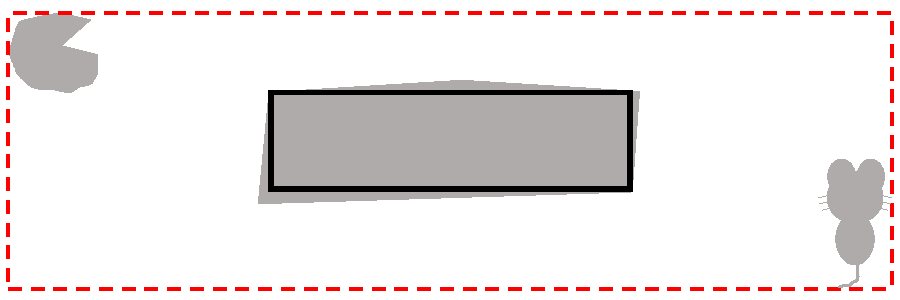
\includegraphics[width=3in]{fig.pdf}
\caption{Example where the underlying distribution $p$ is uniform over the (gray) valid regions. The solid rectangle maximizes our objective since it does not output nonsense (is supported only within the grey matter) and is closest to the $p$ (covers the maximum amount of grey matter). In contrast, the standard maximum likelihood (dashed red) rectangle must fully contain the observed samples, thus generating invalid points most of the time.  }
\end{figure}

Motivated by these observations, we evaluate a generative model $q$ on two axes. First is {\em coverage}, which is related to the probability assigned to future examples drawn from the true distribution $p$. Second is {\em validity}, defined as the probability that random examples generated from $q$ meet some validity requirement. Formally, we measure coverage in terms of a bounded {\em loss}:
$$\Loss(p,q)=\E_{x \sim p}[L(q_x)],$$
where $L:[0,1]\rightarrow [0,M]$ is a bounded decreasing function such as the capped log-loss $L(q_x)=\min(M, \log 1/q_x)$. % or $L(q_x)=\log 1/(q_x+\exp(-M))$. 
A bounded loss has the advantages of being efficiently estimable, and also it enables a model to assign 0 probability to one example (e.g., an outlier or error) if it greatly increases the likelihood of all other data. Validity is defined with respect to a set $V \subseteq X$, and $q(V)$ is the probability that a random example generated from $q$ lies within $V$. 

Clearly, there is a tradeoff between coverage and validity. We first focus on the case of (near) perfect validity. A Valid Generative Modeling (VGM) algorithm if it outputs, for a family of distributions $Q$ over $X$, if it outputs $\hat{q}$ with (nearly) perfect validity and whose loss is nearly as good as the loss of the best valid $q\in Q$. More precisely, $A$ is a VGM learner of $Q$ if for any nonempty valid subset $V \subseteq X$, any probability distribution $p$ over $V$, and any $\eps>0$, $A$ uses $n$ random samples from $p$ and makes $m$ membership oracle calls to $V$ and outputs a distribution $\hat{q}$ such that, $$\Loss(p, \hat{q}) \leq \min_{q \in Q: q(V)=1}\Loss(p,q) + \eps ~\text{ and }~\hat{q}(V)\geq 1-\eps.$$ 
We aim for our learner to be sample and query efficient, requiring that $n$ and $m$ are polynomial in $M, 1/\eps$ and a measure of complexity of our distribution class $Q$.
Furthermore, we would like our algorithms to be computationally efficient, with a runtime polynomial in the size of the data, namely the $n + m$ training examples. 
A more formal description of the problem is available in Section~\ref{sec:problem}.

$A$ is said to be {\em proper} if it always outputs $\hat{q}\in Q$ and {\em improper} otherwise.
In Section~\ref{sec:impossibility}, we first show that efficient proper learning for VGM is impossible. This is an information-theoretic result, meaning that even given infinite runtime and positive samples, one still cannot solve the VGM problem. Interestingly, this is different from binary classification, where it is possible to statistically learn from iid examples without a membership oracle.

Our first main positive result is an efficient (improper) learner for VGM. The algorithm relies on a subroutine that solves the following {\em Generative Modeling with Negatives} (GMN) problem: given sets $X_P, X_N \subset X$ of positive and negative examples, find the probability distribution $q \in Q$ which minimizes $\sum_{x \in X_P} L(q(x))$ subject to the constraint that $q(X_N)=0$. For simplicity, we present our algorithm for the case that the distribution family $Q$ is finite, giving sample and query complexity bounds that are logarithmic in terms of $|Q|$. However, as we show in Section~\ref{sec:infinite-families}, all of our results extend to infinite families $Q$. It follows that if one has a computationally efficient algorithm for the GMN problem for a distribution family $Q$, then our reduction gives a computationally efficient VGM learning algorithm for $Q$.

Our second positive result is an algorithm that minimizes $\Loss(p,q)$ subject to a relaxed validity constraint comparing against the optimal distribution that has validity $q(V)$ at least $1-\alpha$ for some $\alpha>0$. We show in Section~\ref{sec:partial-validity} that even in this more general setting, it is possible to obtain an algorithm that is statistically efficient but may not be computationally efficient. An important open question is whether there exists a computationally efficient algorithm for this problem when given access to an optimization oracle, as was the case for our algorithm for VGM.

\subsection{Related Work}
\cite{KearnsMRRSS94} showed how to learn distributions from positive examples in the realizable setting, i.e., where the true distribution is assumed to belong to the class being learned. In the same sense as their work is similar to PAC learning \citet{Valiant84} of distributions, our work is like agnostic learning \citet{KearnsSS94} in which no assumption on the true distribution is made. 

Generative Adversarial Networks (GANs)~\cite{GoodfellowPMXWOCB14} are an approach for generative modeling from positive examples alone, in which a generative model is trained against a discriminator that aims to distinguish real data from generated data. In some domains, GANs have been shown to outperform other methods at generating realistic-looking examples. Several shortcomings of GANs have been observed \citet{AroraRZ18}, and GANs are still subject to the theoretical limitations we argue are inherent to any model trained without a validity oracle. 

In supervised learning, there is a rich history of learning theory with various types of queries, including membership which are not unlike our (in)validity oracle. Under various assumptions, queries have been shown to facilitate the learning of complex classes such as finite automata \citet{Angluin88} and DNFs \citet{Jackson97}. See the survey of \cite{Angluin92} for further details.  Interestingly, \cite{Feldman09} has shown that for agnostic learning, i.e., without making assumptions on the generating distribution, the addition of membership queries does not enhance what is learnable beyond random examples alone. 
Supervised learning also has a large literature around active learning, showing how the ability to query examples reduces the sample complexity of many algorithms. See the survey of \cite{Hanneke14}. Note that the aim here is typically to save examples and not to expand what is learnable.
 
More sophisticated models, e.g., involving neural networks, can mitigate the invalidity problem as they often generate more realistic natural language and have even been demonstrated to generate \LaTeX{} that nearly compiles \citep{Karpathy15} or nearly valid Wikipedia markdown. However, longer strings generated are unlikely to be valid. For example, \cite{Karpathy15} shows generated markdown which includes:
\begin{quote}
==Access to ''rap===
The current history of the BGA has been [[Vatican Oriolean Diet]], British Armenian, published in 1893.  While actualistic such conditions such as the [[Style Mark Romanians]] are still nearly not the loss.
\end{quote}

Even ignoring the mismatched quotes and equal signs, note that this example has two so-called ``red links'' to two pages that do not exist. Without checking, it was not obvious to us whether or not Wikipedia had pages titled {\em Vatican Oriolean Diet} or {\em Style Mark Romanians}. In some applications, one may or may not want to disallow red links. In the case that they are considered valid, one may seek a full generative model of what might plausibly occur inside of brackets, as the neural network has learned in this case. If they are disallowed, a model might memorize links it has seen but not generate new ones. A validity oracle can help the learner identify what it should avoid generating.

 In practice, \cite{KusnerPH17} discuss how generative models from neural networks (in particular autoencoders) often generate invalid sequences. 
\cite{JanzWPKH18} learn the validity of examples output by a generative model using oracle feedback. 

%!TEX root = LWM_colt.tex
\section{Results}
\label{sec:results}

    In this work, we consider both the specific problem of estimating linear dynamical systems, and a more general problem of linear estimation in time series.
    In both cases we measure the estimation error in the operator norm $\|\cdot\|_{\op}$.
    In Section~\ref{sec:linear_systems} we present upper bounds on the estimation error of the 
parameters $\Ast$ of a linear dynamical system, which hold for any $\Ast$ with $\rho(\Ast) \leq 1$.
%
In Section~\ref{sec:lower_bounds} we show that these upper bounds are
nearly optimal in many regimes of interest.
%
Finally, Section~\ref{sec:meta_thm} states a general result,
which applies to covariate processes with linear responses. 

\textbf{Notation:} We let $\calS^{d-1}$ denote the unit sphere in $\R^d$. Given a matrix $M$ we denote by $M^\dagger$ its pseudoinverse. For a symmetric matrix $M \in \R^{d\times d}$, we let $\lambda_{\max}(M)$ and $\lambda_{\min}(M)$ denote its largest and smallest eigenvalues. If $M \in \R^{d \times d}$ and $M \succ 0$, we denote by $\calS_M$ the set of all points $x\in \R^d$ such that $\|M^{-1/2}x\|_2 = 1$.  


\subsection{Linear Dynamical Systems}
\label{sec:linear_systems}

We analyze the statistical performance of the $\OLS$ estimator of the parameter $\Ast$
    from a single observed trajectory $X_1, \ldots, X_{T+1}$ satisfying $X_{t + 1} = \Ast X_t + \noise_t$, where $X_0 = 0$ and $\noise_t \iid \calN(0, \sigma^2 I_d)$:
    \begin{align}
    \ALS(T) &:= \arg\min_{A \in \R^{d \times d}} \sum_{t=1}^T \frac{1}{2}\|X_{t + 1} - A X_t\|_2^2 \:.
    \end{align}
%
Our bounds are stated in terms of the finite-time controllability Gramian of the system, denoted by $\Gramm_t := \sum_{s=0}^{t-1} (\Ast^{s})(\Ast^s)^{\top}$, which captures the magnitude of the excitations induced by the process noise. Indeed, we can write $X_t$ explicitly as
\begin{eqnarray}\label{eq:recursion_eq}
X_{t} = \sum_{s=1}^{t} \Ast^{t-s}\noise_{s-1}~~\text{ which implies that}~~\Exp[X_tX_t^{\top}] = \sigma^2\Gramm_t~.
\end{eqnarray}
Hence, the expected covariance can be expressed in terms of the Gramians via $\Exp[\sum_{t=1}^T X_tX_t^\top] = \sigma^2\cdot \sum_{t=1}^T \Gramm_t$. As is standard in analyses of least-squares, ``larger'' covariates/covariance matrices correspond to faster rates of learning.
% For example,, and hence, $\Exp\|X_t\|_2^2 = \tr\left(\Gramm_t\right)$. Furthermore, the identity implies th
We are ready to state our first result, proved in Section~\ref{sec:pf_stable_thm}:

\begin{thm}\label{stable_thm} Fix $\delta \in (0,1/2)$ and consider the linear dynamical system $X_{t+1} = \Ast X_t + \noise_t $, where $\Ast$ is a marginally stable matrix in $\R^{d\times d}$ (i.e. $\rho(\Ast) \leq 1$), $X_0 = 0$, and $\noise_t  \iid \calN(0,\sigma^2 I)$. Then there exist universal constants $c,C > 0$ such that
\begin{align}
\Pr\left[\opnormbig{\ALS(T)-\Ast} >\frac{C}{\sqrt{T\lambda_{\min}\left(\Gramm_{k}\right)}} \sqrt{d\log\frac{d}{\delta} + \log \det (\Gramm_T \Gramm_k^{-1})} \right] \le  \delta,
\end{align}
for any $k \ge 1$ such that $\frac{T}{k} \ge c(d\log(d/\delta)+\log \det (\Gramm_T \Gramm_{k}^{-1}))$ holds.
\end{thm}
Note that $\sigma^2$ does not appear in the bound from Theorem~\ref{stable_thm} because scaling the noise also rescales the covariates. In Appendix~\ref{sec:appendix:kst}, we show that for any marginally stable $\Ast$,
we can always choose a $k \geq 1$ provided $T$ is sufficiently large. Therefore, even when $\rho(\Ast) = 1$ and the system does not mix, we obtain finite-sample estimation guarantees which also guarantees consistency of estimation. In many cases, these rates are qualitatively no-worse than random-design linear regression with independent covariates (Theorem~\ref{cor:consistent} and Remark~\ref{rem:consistent}).

In general, $\lambda_{\min}\left(\Gramm_k\right)$ is a nondecreasing function of the block length $k$. The intuition for this is that larger $k$ takes into account more long-term excitations to lower bound the size of our covariance matrix. However, as we use longer blocks, our high probability bounds degrade. Thus, the optimal block length is the maximal value $k$ which satisfies the condition in Theorem~\ref{stable_thm}.

The dependence on the minimum eigenvalue of the Gramian $\lambda_{\min}\left(\Gramm_k\right)$ has two interpretations. From a \emph{statistical} perspective, we have $\frac{1}{2k\cdot \sigma^2}\Exp[\sum_{t=1}^{2k} X_tX_t^\top] = \frac{1}{2k}\sum_{t= 1}^{2k}\Gramm_t \succeq \frac{1}{2}\lambda_{\min}\left(\Gramm_k\right) \cdot I $. Thus, $\lambda_{\min}\left(\Gramm_k\right)$ gives a lower bound on the smallest eigenvalue value of the covariance matrix associated with the first $2k$ covariates. In fact, one can also show (see~\eqref{eq:paley_zygmund}) that for any $t_0 \ge 0$, we still have $\frac{1}{2k\cdot \sigma^2}\Exp[\sum_{t=t_0 + 1}^{t_0 + 2k} X_tX_t^\top | X_{t_0}]~\succeq  \frac{1}{2}\lambda_{\min}\left(\Gramm_k\right) \cdot I$. Theorem~\ref{stable_thm} thus states that the larger the expected covariance matrix, the faster $\Ast$ is estimated. Note that $\Gamma_k \succeq I$ for all $k \ge 1$.

The second interpretation is \emph{dynamical}. The term $\lambda_{\min}\left(\Gramm_k\right)$ corresponds to the ``excitability'' of the system, which is the extent to which the process noise $\noise_t$ influences future covariates. This can be seen from~\eqref{eq:recursion_eq}, where the slower $(\Ast^{t_0})(\Ast^{t_0})^\top$ decays as $t_0$ grows, the larger the contribution of $\noise_{t - t_0-1}$ is. This is precisely the reason why linear systems with larger spectral radii mix slowly, and do not mix when $\rho(\Ast) \ge 1$.
%
In this light, Theorem~\ref{stable_thm} shows that with high-probability, the more a linear system is excited by the noise $\noise_t$, the easier it is to estimate the parameter matrix $\Ast$. For stable systems with $\rho(\Ast) < 1$, the following corollary removes the explicit dependence on the block length $k$ for large values of $T$:
\begin{cor}\label{cor:mixed_cor}
Suppose that $\rho(\Ast) < 1$. Then the limit $\Gamma_{\infty} := \lim_{t \to \infty} \Gamma_t$ exists, and there is a time $T_0$ depending on $\Ast$ and $\delta$ such that the following holds w.p. $1-\delta$ for all $T > T_0$:
\begin{eqnarray}
\opnormbig{\ALS(T)-\Ast} \le \BigOh{\sqrt{ \frac{d \cdot \log\left(\frac{d}{\delta} \right)}  {T\lambda_{\min}\left(\Gramm_{\infty}\right)}}}  \,.
\end{eqnarray}
\end{cor}
The above corollary uses the fact that $\lim_{k \to \infty}\|\Ast^k\|_{\op}^{1/k} = \rho(\Ast)$, which implies that the limit $\lim_{t \to \infty} \Gamma_t$ is finite when $\rho(\Ast) < 1$. The rate of the convergence of $\Gamma_t$ to $\Gamma_{\infty}$ is related to the $\mathcal{H}_{\infty}$-norm of the linear system, a core concept in control theory. For an extended discussion on this relationship, we direct the reader to~\cite{tu2017non}. Corollaries~\ref{cor:consistent} and~\ref{cor:diag} in the appendix give an analogue of Corollary~\ref{cor:mixed_cor} which holds even if $\rho(\Ast) = 1$. We now explicitly describe the consequences of Theorem~\ref{stable_thm} for three illustrative classes of linear systems:

%Even a when $\rho(A^*) = 1$, we can find a positive block length $k$ which satisfies the hypothesis of Theorem~\ref{stable_thm}, provided $T$ is sufficiently large.

\begin{enumerate}
\item \textbf{Scalar linear system.} In this case the states $X_t$ and the parameter $\Ast$ are scalars, and denoted $a_* = \Ast$. For $|a_*| \le 1$, we can apply Theorem~\ref{stable_thm} with block length $k = \BigOm(T/\log(1/\delta))$. This then guarantees that $|\widehat{a} - a_*| \leq \BigOm\left(\sqrt{\log(1/\delta)/\left(T \sum_{t = 1}^{k_*} a_*^{2t} \right)}\right)$ with probability $1 - \delta$. In Appendix~\ref{sec:1d_appendix}, we show this statistical rate is minimax optimal (Theorem~\ref{thm:info_lb_1d}). Moreover, we offer a specialized analysis for the scalar case (Theorem~\ref{thm:one_d_thm}) which yields sharper constants and also applies to the unstable case $|a_*| > 1$, matching the lower bounds of Theorem~\ref{thm:info_lb_1d}. Stated succinctly, our results in Appendix~\ref{sec:1d_appendix} imply that the $\OLS$ estimator satisfies with probability $1 - \delta$ error guarantees which can be categorized into three regimes:
\begin{align*}
    |\widehat{a} - a_*| = \begin{cases}
        \Theta\left(\sqrt{\frac{\log(1/\delta)(1 - |a_*|)}{T}}\right)\; &\text{ if }\; |a_*| \leq 1 - \frac{c\log(1/\delta)}{T},\\
        \Theta\left(\frac{\log(1/\delta)}{T}\right)\; &\text{ if }\; 1 - \frac{c\log(1/\delta)}{T} < |a_*| \leq 1 + \frac{1}{T}\\
        \Theta\left(\frac{\log\left(1/\delta\right)}{|a_*|^T}\right) \; &\text{ if }\; 1 + \frac{1}{T} \le |a_*|.
    \end{cases}
\end{align*}

\citet{white1958limiting} showed the same dependence on $|a_*|$ of the estimation error by characterizing the asymptotic distribution of $\widehat{a} - a_*$ when appropriately scaled. However, our results offer finite sample guarantees. 


\item \textbf{Scaled orthogonal systems.} Let us assume $\Ast =  \rho \cdot O$ for an orthogonal $d\times d$ matrix $O$ and $|\rho| \leq 1$. Then, one can verify that $\Gamma_t = I \cdot \sum_{s=0}^{t-1} \rho^{2s}$ and that we can choose the block length $k = \BigOm\left(\tfrac{T}{d\log(d/\delta)}\right)$. Therefore, Theorem~\ref{stable_thm} guarantees that with probability $1 - \delta$:
\begin{align}\label{eq:rho_eye_upper}
\opnorm{\ALS - \Ast} \leq \begin{cases}
    \BigOm\left(\sqrt{(1-|\rho|) \cdot \frac{d\log(d/\delta)}{T}}\right)\; &\text{ if }\; |\rho| \leq 1 - \frac{cd\log(d/\delta)}{T},\\
    \BigOm\left(\frac{d\log(d/\delta)}{T}\right)\; &\text{ if }\; 1 - \frac{cd\log(d/\delta)}{T} < |\rho|.
\end{cases}
\end{align}

	\item \textbf{Diagonalizable linear systems.} Let $\Ast = SDS^{-1}$ define a diagonalizable linear system. We denote by $\underline{\rho}$ the smallest magnitude of an eigenvalue of $\Ast$. In Appendix~\ref{app:consistent}, we show that we can choose the block length $k$ such that
$
k \geq \frac{T}{c d \log\left(\frac{d \, \cond(S)}{\delta}\right)}. 
$
With this choice of $k$ the $\OLS$ estimator satisfies (Corollary~\ref{cor:diag})
\begin{align*}
\Pr\left[\opnorm{\ALS - \Ast} \leq \BigOm\left(\sqrt{\frac{d\log(d \, \cond(S)/\delta)}{T\left(1 + \cond(S)^{-2}\sum_{s = 0}^{k-1}\underline{\rho}^{2s}\right)}}\right)\right] \ge 1- \delta
\end{align*}
which could once again be split into a slow and fast rate, as in the examples presented above, depending on the size $\underline{\rho}$ of the least excitable mode of the system defined by $\Ast$. Note that up to a factor of $\log(d \, \cond(S)/\delta)$, the above bound is no worse than the worst-case rate for standard random-design least-squares in the operator norm (see Appendix~\ref{app:op_norm_ls}).
\end{enumerate}
\begin{remark}[Noise dependence] As mentioned before, the estimation guarantee provided by Theorem~\ref{stable_thm} does not depend on the variance $\sigma^2$ of the noise $\noise_t$. For Gaussian noise with a general identity covariance $\noise_t \sim \calN(0,\Sigma)$, one can rederive rates from our more general Theorem~\ref{main_thm} to get a more precise dependence on $\Gramm_t$ and $\Sigma$.
%
Note that if the covariance $\Sigma$ is known, an alternative estimator would be to choose $\ALS$ to minimize a loss which takes $\Sigma$ into account in the same way that one would for non-dynamic linear regression with heteroskedastic noise, e.g. $\widehat{A}^{\Sigma}(T) := \arg\min_{A \in \R^{d \times d}} \sum_{t=1}^T \frac{1}{2}\left\|\Sigma^{-1/2}\left(X_{t + 1} - A X_t\right)\right\|_2^2$.
\end{remark}
\begin{remark}[Learning with input sequences] We can also consider the case where the linear system $X_{t + 1} = \Ast X_t + \Bst u_t + \eta_t$ is driven by a known sequence of inputs $u_0,u_1,\dots$, with known $\Bst$. Defining the control Gramian $\GrammB_t := \sum_{s=1}^t \Ast^{t-s}\Bst\Bst^\top \Ast^{t-s}~$, the proof of Theorem~\ref{stable_thm} can be modified to show that, if the inputs are white noise $u_t \overset{i.i.d}{\sim} \mathcal{N}(0,\sigmaU^2 I)$, then there exist universal constants $c,C > 0$ such that, with probability $1-\delta$,
\begin{align*}
\opnorm{\ALS(T)-\Ast} \le \frac{C\sigma^2}{\sqrt{T\lambda_{\min}\left(\sigma^2\Gramm_k + \sigmaU^2 \GrammB_k)\right)}}\sqrt{d\log\left(\frac{1}{\delta} \frac{\tr \left(\sigma^2\Gramm_T + \sigmaU^2 \GrammB_T)\right)}{\lambda_{\min}\left(\sigma^2\Gramm_k + \sigmaU^2 \GrammB_k\right)}\right)}
\end{align*}
for any $k$ such that $\frac{T}{k} \ge cd\log \left( \frac{\tr(\sigma^2\Gramm_T + \sigmaU^2 \GrammB_T)}{\delta\lambda_{\min}(\sigma^2\Gramm_k + \sigmaU^2 \GrammB_k)} \right)$. Process noise with covariance not equal to a multiple of the identity can be absorbed into $\Bst$. 
\end{remark}

\subsection{Lower Bounds for Linear System Identification}
\label{sec:lower_bounds}

    We have seen in Theorem~\ref{stable_thm} and in the subsequent examples that the estimation of linear dynamical systems is easier for systems
    which are easily excitable. It is natural to ask what is the best possible estimation rate one can hope to achieve. To make explicit the dependence of the lower bounds on the spectrum of $\Gamma_t$, we consider the minimax rate of estimation over the set $\eig \cdot \Od$, where $\eig \in \R$ and $\Od$ denotes the orthogonal group. In this case, we can define an \emph{scalar} Gramian $\gamma_t(\eig) := \sum_{s=0}^{t-1} |\eig|^{2s}$, so that $\Gamma_t := \gamma_t(\eig) \cdot I$. We now show that the estimation rate of the $\OLS$ provided in Theorem~\ref{stable_thm} is optimal up to log factors for $|\rho| \le 1 - \BigOhTil{d/T}$:
    \begin{thm}
    \label{thm:info_lb_d} Fix  $d \ge 2$, $\eig \in \R$, $\delta \in (0,1/4)$, and $\epsilon \le \frac{\eig}{2048}$. Then, there exists a universal constant $c_0$ such for any estimator $\widehat{A}$,
    \begin{eqnarray*}
    \sup_{O \in \Od}\Pr_{\eig O}\left[\left\|\widehat{A}(T) - \eig O\right\|_{\op} \ge \epsilon\right] \ge \delta\; \text{ for any } T \text{ such that }\; T \gamma_{T}(\eig) \leq  \frac{c_0 \left( d + \log\left(1/\delta\right)\right)}{\epsilon^2},
    \end{eqnarray*}
    where $\Od$ is the orthogonal group of $d \times d$ real matrices.
    \end{thm}
    This result is proved in Appendix~\ref{sec:lb_proofs}. We can interpret it
    by considering the following regimes:
\begin{align*}
    \opnorm{\widehat{A} - \Ast} \ge \begin{cases}
        \Omega\left(\sqrt{\frac{(d+\log(1/\delta))\cdot(1 - |\rho|)}{T}}\right)\; &\text{ if }\; |\rho| \leq 1 - \frac{1}{T},\\
        \Omega\left(\frac{\sqrt{d+\log(1/\delta) }}{T}\right)\; &\text{ if }\; 1 - \frac{1}{T} < |\rho| < 1 + \frac{1}{T}\\
        \Omega\left(\frac{\sqrt{d+\log(1/\delta)}}{T|\rho|^T}\right) \; &\text{ if }\; 1 + \frac{1}{T} \le |\rho|.
    \end{cases}
\end{align*}
Comparing to~\eqref{eq:rho_eye_upper}, we see that for $|\rho| \le 1 - \BigOhTil{d/T}$, our upper and lower bounds coincide up to logarithmic factors. In the regime $\rho \in [1 - \BigOhTil{d/T},1]$, our upper and lower bounds differ by a factor of $\BigOhTil{\sqrt{d + \log(1/\delta)}}$. 

%We conjecture that our upper bounds qualitatively describe the performance of $\OLS$; that we conjecture that the least-squares estimator actually attains a rate of $\BigOh{\frac{d + \log(1/\delta)}{T}}$ (without the log factors) and that our lower bounds are off by a factor of $\BigOhTil{\sqrt{d + \log(1/\delta)}}$.\horia{Not sure what we are trying to conjecture here, but something is wrong.}

%; we provide a heuristic argument which is specific to least squares in Appendix~\ref{sec:Lower_Bound_Loose}. It is possible that shaving off the $\BigOhTil{\sqrt{d + \log(1/\delta)}}$ factor for $|\rho|$ close to one may be informational-theoretically possible (that is, attainable by an algorithm other than OLS).


% \subsection{Estimation Rates with Known $\Bst$}
% In this section, we show that the learning rates can be improved when the system is driven by inputs $u_t$ when the control matrix $\Bst$ is known. For ease, we assume that the inputs are white noise $u_t \overset{i.i.d}{\sim} \mathcal{N}(0,\sigmaU^2 I)$. In this regime, note that we have the decomposition:
% \begin{eqnarray}\label{eq:recursion_eq}
% &&X_{t+1} = \sum_{s=1}^{t} \Ast^{t-s}(\noise_s+\Bst u_t)~~\text{ which implies that}~~\Exp[X_tX_t^{\top}] = \sigma^2\Gramm_t~ + \sigmaU^2 \GrammB_t~,\nonumber\\
% \text{where}&& \quad \GrammB_t := \sum_{s=1}^t \Ast^{t-s}\Bst\Bst^\top \Ast^{t-s}~.
% \end{eqnarray}
% With these definitions, we can now state an analogue of Theorem~\ref{stable_thm} for control inputs, which is again a consequence of Theorem~\ref{main_thm}:
% \begin{thm}\label{thm:stbl_input} Fix $\delta \in (0,1/2)$ and consider the linear dynamical system $X_{t+1} = \Ast X_t + \Bst u_t + \noise_t $, where $\Ast$ is a marginally stable matrix in $\R^{d\times d}$, $X_0 = 0$, $\noise_t  \iid \calN(0,\sigma^2 I)$, and $u_t \sim \mathcal{N}(0,\sigmaU^2 I)$.
% \end{thm}



\subsection{General Time Series with Linear Responses}
\label{sec:meta_thm}

    In this section, we consider a sequence of covariate-response pairs $(X_t,Y_t)_{t \ge 1}$, where $Y_t = \Ast X_t + \noise_t$, with $Y_t, \noise_t \in \R^n$, $X_t \in \R^d$, and $\Ast \in \R^{n \times d}$. The least squares estimator is then
    \begin{eqnarray}
    \ALS(T) &:= \arg\min_{A \in \R^{d \times d}} \sum_{t=1}^T \frac{1}{2}\|Y_{t} - A X_t\|_2^2 \:.
    \end{eqnarray}

    We let $\calF_{t} := \sigma(\noise_0,\noise_1,\dots,\noise_{t},X_1,\dots,X_t)$ denote the filtration generated by the covariates and noise process. Note then that $Y_t \in \calF_{t}$, but $Y_t \notin \calF_{t - 1}$. Further, we assume $\eta_t | \calF_{t-1}$ is mean-zero, and $\sigma^2$-sub-Gaussian (i.e., $\Exp[\exp(\lambda \eta_t) | \calF_t] \le e^{\sigma^2 \lambda^2/2}$).
    %
    The linear dynamical systems sub-case is recovered from this general setting when $Y_t = X_{t+1}$.

%For concreteness, the $\OLS$ estimates for the two cases considered here are respectively
%
%
%    \begin{align}
%    \label{eq:ols}
%    \ALS(T) &:= \arg\min_{A \in \R^{n \times d}} \sum_{t=1}^T \frac{1}{2}\|Y_t - A X_t\|_2^2.
%    \end{align}

%	In this section, we analyze the performance of the $\OLS$ estimator when applied to time series of the form $Y_t = \Ast X_t + \noise_t$.
%
% Theorem~\ref{stable_thm} is a consequence of the result presented in this section.
    To capture the excitation behavior observed in the case of linear systems we introduce a general martingale small-ball condition which quantifies the growth of the covariates $X_t$.
	\begin{defn}[Martingale Small-Ball]\label{def:bmsb} Let $(Z_t)_{t \ge 1}$ be an $\{\calF_t\}_{t \ge 1}$-adapted random process  taking values in $\R$. We say $(Z_t)_{t\ge 1}$ satisfies the $(k,\nu,p)$-block martingale small-ball (BMSB) condition if, for any $j \ge 0$, one has $\frac{1}{k}\sum_{i=1}^k \Pr( |Z_{j+i}| \ge \nu | \calF_{j}) \ge p$ almost surely.  Given a process $(X_t)_{t \ge 1}$ taking values in $\R^d$, we say that it satisfies the $(k,\Gamsb,p)$-BMSB condition for $\Gamsb \succ 0$ if, for any fixed $w\in \calS^{d-1}$, the process $Z_t:= \langle w, X_t\rangle$ satisfies $(k,\sqrt{w^\top \Gamsb w},p)$-BMSB.
	\end{defn}

	Such a small-ball condition is necessary for establishing a high-probability lower bound on $\lambda_{\min}(\sum_{t=1}^T X_tX_t^\top) = \min_{\direc \in \calS^{d-1}} \sum_{t=1}^T \langle X_t, \direc \rangle^2$. The parameter $\Gamsb$ plays the role of the Gramians $\Gramm_t$ considered in the case of linear systems,
    and measures how excitable the covariates $X_t$ are. As expected, the next result shows that a higher $\lambda_{\min}(\Gamsb)$ leads to faster statistical estimation.

\begin{thm}\label{main_thm} Fix $\epsilon, \delta \in (0,1)$, $T \in \N$ and $0 \prec \Gamsb \preceq \Gambar$. Then if $(X_t,Y_t)_{t \ge 1} \in (\R^d \times \R^n)^{T}$ is a random sequence such that (a) $Y_t = \Ast X_t + \noise_t$, where $\noise_t | \calF_t$ is $\sigma^2$-sub-Gaussian and mean zero, (b) $X_1,\dots,X_T$ satisfies the $(k,\Gamsb,p)$-small ball condition, and (c) such that\\ $\Pr[\sum_{t = 1}^T X_t X_t^\top \npreceq T\Gambar] \le \delta$. Then if 
\begin{align}\label{eq:main_thm_condition}
T \geq  \frac{10k}{p^2}\left(\log \left(\frac{1}{\delta}\right) + 2d\log(10/ p) +  \log \det (\Gambar \Gamsb^{-1}) \right),
\end{align}
we have
\begin{align}
\Pr\left[\opnormbig{\ALS(T)-\Ast} >\frac{90\sigma}{p}\sqrt{\frac{n + d\log \frac{10}{p} + \log \det \Gambar \Gamsb^{-1} + \log\left(\frac{1}{\delta}\right)}{T\lambda_{\min}(\Gamsb)}} \right] \le  3\delta.
\end{align}
\end{thm}
%\begin{remark}
The proof of Theorem~\ref{main_thm} is outlined in Section~\ref{sec:mn_thm_proof}, and technical details are deferred to Appendix~\ref{app:main_thm}. We remark that the conclusion of Theorem~\ref{main_thm} still holds if one replaces the $(k,\Gamsb,p)$ small-ball condition with any high probability lower bound of the form $\Pr\left( \sum_{t = 1}^T X_t X_t^\top \succsim T \Gamsb \right) \leq \delta$.
%\end{remark}

\subsection{Analysis Techniques\label{sec:analysis_tech}}
Let $\ALS = \ALS(T)$, let $\matX \in \R^{T \times d}$ denote the matrix whose rows are $X_t$, and $\Noise \in \R^{T \times n}$ denote the matrix
whose rows are $\noise_t$.  Consider the compact SVD of $\matX$ and
$\matX = \matU \matSig \matV^\top$, where $\matSig,\matV \in \R^{d \times d}$
and $\matU \in \R^{T \times d}$. Note then that we have $\ALS - A_* =
(\matX^{\dagger} \Noise)^\top $ which implies that
\begin{eqnarray}\label{eq:error_decomp}
\opnorm{\ALS - A_\star}  = \opnorm{\matX^{\dagger} \Noise} \leq \sigma_{d}(\matX)^{-1}\opnorm{\matU^{\top}\Noise}.
\end{eqnarray}
Here $\sigma_{d}((\matX)^{-1})$ denotes the $d$-th largest singalue value of $\matX$, which is precisely $\sqrt{1/\lambda_{\min}(\matX^\top \matX)}$.
The technical challenge arises from the fact that the singular space $\matU^{\top}$ and $\Noise$ are correlated, and that the rows $X_t$ of $\matX$ are also dependent. We upper bound $\opnorm{\matU^{\top}\Noise}$ with Lemma~\ref{eq:normalized}, a martingale-Chernoff bound that gives precise control on the deviations of sub-Gaussian martingale sequences in terms of random variance proxies. We explain this argument in more detail at the end of Section~\ref{sec:mn_thm_proof}.

Our lower bound on $\sigma_{\min}(\matX) = \sqrt{\lambda_{\min}(\sum_{t=1}^TX_tX_t^\top)}$ eschews mixing-time arguments in favor of a careful modification of Mendelson's small-ball method~\citep{mendelson14b}. %to lower bound the least singular value of the covariance matrix $\sum_{t=1}^T X_tX_t^\top$.
We divide our covariates into size-$k$ blocks $\{X_{(\ell-1) k + 1},\dots,X_{\ell k}\}$, such that for  any fixed $\direc \in \calS^{d-1}$, the quantity $\sum_{\ell=1}^k \langle X_{(\ell-1) k + 1}, \direc \rangle^2$ can be lower bounded by the $(k, \Gamsb, p)$-BMSB condition. Proposition~\ref{prop:Small_Ball} below (proved in Appendix~\ref{sec:proof_small_ball}) then implies that we have $\sum_{t=1}^T \langle X_t, \direc \rangle^2~\gtrsim~T w^\top \Gamsb w$~with probability at least $1 - \exp( - c T/k)$ for some constant $c$:
\begin{prop}\label{prop:Small_Ball} Let $\{Z_t\}_{t\geq 1}$ be  a scalar process  that satisfies the $(k,\nu,p)$-BMSB condition. Then
    \begin{eqnarray}
    \Pr\left[\sum_{i=1}^T Z_i^2 \le \frac{\nu^2p^2}{8} k\floor{T/k}\right] \leq   e^{-\frac{\floor{T/k}p^2}{8}}.
    \end{eqnarray}
 \end{prop}
Once $T$ is large enough, these high-probability bounds can be used to derive a uniform bound over $\direc \in \calS^{d-1}$ via a discretization argument (Lemma~\ref{lem:eig_Packing_Lem}).  In general there is a trade-off between the size of the blocks $k$ and the probability guarantee obtained: a larger block size leads to a larger
parameter $\nu$ and a faster rate, but it degrades the probability guarantee.

 %e show that in the case of linear systems, this trade-off can be settled to yield fast rates of estimation for nearly unstable matrices $\Ast$ which hold with high probability.


  %	\maxs{explain: advantage is that we need failure probability $e^{-\BigOhTil{d}}$ for lb on $\sigma_{\min}(\dots)$, so we can have as few as $T/\BigOhTil{d}$-blocks. And fewer blocks means large $k$ means large $\nu$, necessarily bc we can only lower bound with $\nu$ w. const prob, not high prob. }

%%% Local Variables:
%%% mode: latex
%%% TeX-master: t
%%% End:

%!TEX root = main.tex
\vspace{-.0cm}
\section{Preliminaries}\label{sec:background}
\vspace{-1.22pt}
We recall some important concepts from Riemannian geometry. \citet{do2016differential}  provides more a thorough review, with \citet{absil2009optimization} providing a perspective particularly relevant for Riemannian optimization.

As a base space we consider a Riemannian manifold $(\M, \g)$--a smooth manifold equipped with a Riemannian metric $\g$ containing a compact, connected subset $\X$. At all $x \in \M$, the metric $\g$ induces a natural inner product on the tangent space $T_{x} \M$, denoted by $\langle\cdot,\cdot\rangle$--this inner product induces a norm on each tangent space denoted by $\Vert \cdot \Vert$. The metric $\g$ also provides a means of measuring the length of a parametrized curve from $\mathbb{R}$ to the manifold; a \emph{geodesic} is a constant speed curve $\gamma\! :\! [0,1]\! \to\! \M$ that is locally distance-minimizing with respect to the distance~$d$ induced by $\g$.

When considering functions $f : \M \to \mathbb{R}$ we will use $\nabla f(x) \in T_{x} M$ to denote the \emph{Riemannian gradient} of $f$ at $x \in \M$, and $\Hess f(x) : T_{x} M \to T_{x} M$, the \emph{Riemannian Hessian} of $f$ at $x$. When considering functions between manifolds $F : \M \to \M$, we will use $D F(x) : T_{x} \M \to T_{F(x)} \M$ to denote the \emph{differential} of the mapping at $x$ (its linearization) % for which the chain rule and inverse function theorem also hold
\citep[see][for more formal definitions of these objects]{absil2009optimization}.
 \begin{figure}[!t]
 \vspace{-.5cm}
\centering
\begin{minipage}[c]{.48\linewidth}
 \def\svgwidth{2.5in}
%!TEX root = ../colt2018-manifold.tex

%% Creator: Inkscape inkscape 0.92.2, www.inkscape.org
%% PDF/EPS/PS + LaTeX output extension by Johan Engelen, 2010
%% Accompanies image file 'retraction.pdf' (pdf, eps, ps)
%%
%% To include the image in your LaTeX document, write
%%   \input{<filename>.pdf_tex}
%%  instead of
%%   \includegraphics{<filename>.pdf}
%% To scale the image, write
%%   \def\svgwidth{<desired width>}
%%   \input{<filename>.pdf_tex}
%%  instead of
%%   \includegraphics[width=<desired width>]{<filename>.pdf}
%%
%% Images with a different path to the parent latex file can
%% be accessed with the `import' package (which may need to be
%% installed) using
%%   \usepackage{import}
%% in the preamble, and then including the image with
%%   \import{<path to file>}{<filename>.pdf_tex}
%% Alternatively, one can specify
%%   \graphicspath{{<path to file>/}}
%% 
%% For more information, please see info/svg-inkscape on CTAN:
%%   http://tug.ctan.org/tex-archive/info/svg-inkscape
%%
\begingroup%
  \makeatletter%
  \providecommand\color[2][]{%
    \errmessage{(Inkscape) Color is used for the text in Inkscape, but the package 'color.sty' is not loaded}%
    \renewcommand\color[2][]{}%
  }%
  \providecommand\transparent[1]{%
    \errmessage{(Inkscape) Transparency is used (non-zero) for the text in Inkscape, but the package 'transparent.sty' is not loaded}%
    \renewcommand\transparent[1]{}%
  }%
  \providecommand\rotatebox[2]{#2}%
  \ifx\svgwidth\undefined%
    \setlength{\unitlength}{198.42519685bp}%
    \ifx\svgscale\undefined%
      \relax%
    \else%
      \setlength{\unitlength}{\unitlength * \real{\svgscale}}%
    \fi%
  \else%
    \setlength{\unitlength}{\svgwidth}%
  \fi%
  \global\let\svgwidth\undefined%
  \global\let\svgscale\undefined%
  \makeatother%
  \begin{picture}(1,1)%
    \put(0,0){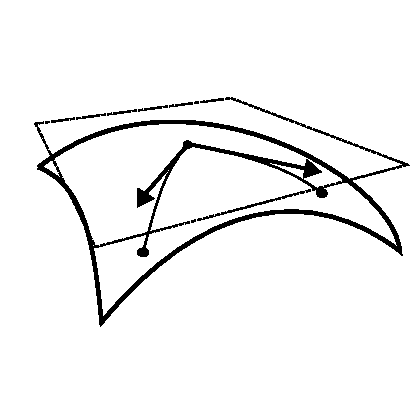
\includegraphics[width=\unitlength,page=1]{Figs/retractionbis.pdf}}%
    \put(0.47046491073,0.658059720226){\color[rgb]{0,0,0}\makebox(0,0)[lb]{\smash{$x_{n-1}$}}}%
     \put(0.75,0.60){\color[rgb]{0,0,0}\makebox(0,0)[lb]{\smash{$-\!\gamma_{n}\nabla f_{n}(x_{n-1})$}}}%
    \put(0.050473214,0.74160431){\color[rgb]{0,0,0}\makebox(0,0)[lb]{\smash{$T_{x_{n-1}}\M$}}}%
    \put(0.88081831845,0.328726181){\color[rgb]{0,0,0}\makebox(0,0)[lb]{\smash{$\M$}}}%
    \put(0.2809223052,0.47167483){\color[rgb]{0,0,0}\makebox(0,0)[lb]{\smash{$v$}}}%
     \put(0.780809223052,0.490167483){\color[rgb]{0,0,0}\makebox(0,0)[lb]{\smash{$x_{n}$}}}%
    \put(0.2207857,0.3651749994){\color[rgb]{0,0,0}\makebox(0,0)[lb]{\smash{$R_{x_{n\!-\!1}}\!(v)$}}}%
  \end{picture}%
\endgroup%

   \end{minipage}
   \begin{minipage}[c]{.48\linewidth}
 \def\svgwidth{2.5in}
%!TEX root = ../colt2018-manifold.tex

%% Creator: Inkscape inkscape 0.92.2, www.inkscape.org
%% PDF/EPS/PS + LaTeX output extension by Johan Engelen, 2010
%% Accompanies image file 'transport.pdf' (pdf, eps, ps)
%%
%% To include the image in your LaTeX document, write
%%   \input{<filename>.pdf_tex}
%%  instead of
%%   \includegraphics{<filename>.pdf}
%% To scale the image, write
%%   \def\svgwidth{<desired width>}
%%   \input{<filename>.pdf_tex}
%%  instead of
%%   \includegraphics[width=<desired width>]{<filename>.pdf}
%%
%% Images with a different path to the parent latex file can
%% be accessed with the `import' package (which may need to be
%% installed) using
%%   \usepackage{import}
%% in the preamble, and then including the image with
%%   \import{<path to file>}{<filename>.pdf_tex}
%% Alternatively, one can specify
%%   \graphicspath{{<path to file>/}}
%% 
%% For more information, please see info/svg-inkscape on CTAN:
%%   http://tug.ctan.org/tex-archive/info/svg-inkscape
%%
\begingroup%
  \makeatletter%
  \providecommand\color[2][]{%
    \errmessage{(Inkscape) Color is used for the text in Inkscape, but the package 'color.sty' is not loaded}%
    \renewcommand\color[2][]{}%
  }%
  \providecommand\transparent[1]{%
    \errmessage{(Inkscape) Transparency is used (non-zero) for the text in Inkscape, but the package 'transparent.sty' is not loaded}%
    \renewcommand\transparent[1]{}%
  }%
  \providecommand\rotatebox[2]{#2}%
  \ifx\svgwidth\undefined%
    \setlength{\unitlength}{198.42519685bp}%
    \ifx\svgscale\undefined%
      \relax%
    \else%
      \setlength{\unitlength}{\unitlength * \real{\svgscale}}%
    \fi%
  \else%
    \setlength{\unitlength}{\svgwidth}%
  \fi%
  \global\let\svgwidth\undefined%
  \global\let\svgscale\undefined%
  \makeatother%
  \begin{picture}(1,1)%
    \put(0,0){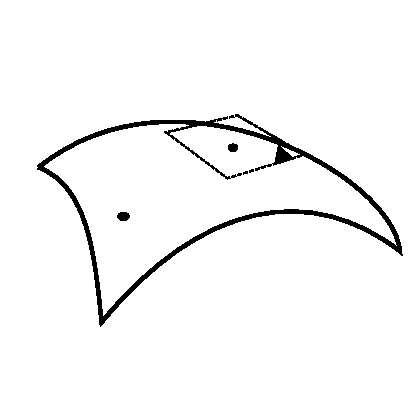
\includegraphics[width=\unitlength,page=1]{Figs/transport2.pdf}}%
    \put(0.88081831845,0.328726181){\color[rgb]{0,0,0}\makebox(0,0)[lb]{\smash{$\M$}}}%
    \put(0,0){\includegraphics[width=\unitlength,page=2]{Figs/transport2.pdf}}%
    \put(0.49373014,0.651988096){\color[rgb]{0,0,0}\makebox(0,0)[lb]{\smash{$x$}}}%
    \put(0.236627,0.47247038){\color[rgb]{0,0,0}\makebox(0,0)[lb]{\smash{$y$}}}%
    \put(0.1720032738,0.6014499){\color[rgb]{0,0,0}\makebox(0,0)[lb]{\smash{$T_y\M$}}}%
    \put(0.594176587,0.7369925609){\color[rgb]{0,0,0}\makebox(0,0)[lb]{\smash{$T_x\M$}}}%
    \put(0.70539679,0.56444469){\color[rgb]{0,0,0}\makebox(0,0)[lb]{\smash{$v$}}}%
    \put(0.42325397,0.4704097231){\color[rgb]{0,0,0}\makebox(0,0)[lb]{\smash{$\tp{x}{y}(v)$}}}%
  \end{picture}%
\endgroup%

  \end{minipage}
  \vspace{-1cm}
\caption{Left: In the tangent space at iterate $x_{n-1}$, a retraction along an arbitrary vector $v$ generating a curve pointing in the ``direction'' of  $v$, and a retraction along the gradient update to $x_n$. Right:
The parallel transport of a different $v$ along the same path.}
\label{fig:manifold}
  \vspace{-.5cm}
\end{figure}
The \emph{exponential map} $\Exp_{x}(v) : T_{x} \M \to \M$ maps $v \in T_{x} \M$ to $y \in \M$ such that there is a geodesic with $\gamma(0)=x$, $\gamma(1)=y$, and $\frac{d}{dt}\gamma(0)=v$; although it may not be defined on the whole tangent space. If there is a unique geodesic connecting $x, y \in \X$, the exponential map will have a well-defined inverse $\Exp_{x}^{-1}(y) : \M \to T_{x}\M$, such that the length of the connecting geodesic is $d(x,y)=\Vert \Exp_{x}^{-1}(y) \Vert$. We also use $R_x : T_{x} \M \to \M$ and $R_x^{-1} : \M \to T_{x}\M$ to denote a \emph{retraction mapping} and its inverse (when well defined), which is an approximation to the exponential map (and its inverse). $R_x$ is often computationally cheaper to compute then the entire exponential map $\Exp_x$. Formally, the map $R_x$ is defined as a first-order retraction if $R_x(0) = x$ and $D R_x(0)= id_{T_{x} \M}$---so locally $R_x(\xi)$ must move in the ``direction'' of $\xi$. The map $R_x$ is a second-order retraction if $R_x$ also satisfies $\frac{D^2}{dt^2} R_x(t \xi)|_{0} = 0$ for all $\xi \in T_{x}\M$, where $\frac{D^2}{dt^2}\gamma = \frac{D}{dt} \dot{\gamma}$ denotes the acceleration vector field \citep[][Sec.~5.4]{absil2009optimization}. This condition ensures $R_x$ satisfies a ``zero-acceleration'' initial condition.
Note that locally, for $x$ close to $y$, the retraction satisfies $\norm{R^{-1}_{x}(y)} = d(x, y) + o(d(x, y))$.

If we consider the example where the manifold is a sphere (i.e., $\M = S^{d-1}$ with the round metric $\g$), the exponential map along a vector will generate a curve that is a great circle on the underlying sphere. A nontrivial example of a retraction $R$ on the sphere can be defined by first moving along the tangent vector in the embedded Euclidean space $\mathbb{R}^d$, and then projecting this point to the closest point on the sphere.

We further define the \emph{parallel translation} $\tp{x}{y} : T_x \mathcal{M} \to T_y \mathcal{M}$ as the map
transporting a vector $v \in T_x \M$ to $\tp{x}{y} v$, along a path $R_{x}(\xi)$ connecting $x$ to $y = R_{x}(\xi)$, such that the vector stays ``constant" by satisfying a zero-acceleration condition. This is illustrated in \myfig{manifold}. The map $\tp{x}{y}$ is an isometry. We also consider, a different vector transport map $\te{x}{y}:T_x \mathcal{M} \to T_y \mathcal{M}$ which is the differential  $DR_{x}(R_x^{-1}(y))$ of the retraction $R$ \citep[][Sec.~8.1]{absil2009optimization}.

Following \citet{huang2015broyden}, we will call a function $f$ on $\X$ \emph{retraction convex} on $\X$ (with respect to $R$) if for all $x \in \X$ and all $\eta \in T_{x}\M$ satisfying $\norm{\eta}=1$, $t \mapsto f(R_{x}(t \eta))$ is convex for all $t$ such that $R_{x}(t \eta) \in \X$; similarly $f$ is \emph{retraction strongly convex} on $\X$ if $t \mapsto f(R_{x}(t \eta))$ is strongly convex under the same conditions. If $R_x$ is the exponential map, this reduces to the definition of geodesic convexity \citep[see the work of][for further details]{zhang2016first}.
\vspace{-1.21pt}
\section{Assumptions} \label{sec:assumptions}
\vspace{-1.22pt}
We introduce several assumptions on the manifold $\M$, function $f$, and the noise process $\{\nabla f_n\}_{n\geq1}$ that will be relevant throughout the paper.
\vspace*{-.1850cm}
\subsection{Assumptions on $\M$}
\vspace{-.0856cm}
First, we assume the iterates of the algorithm in \eq{grad_desc} and \eq{ave_grad_desc}
remain in $\mathcal X$ where the manifold ``behaves well.'' Formally,
\vspace*{-4pt}
\begin{assumption} \label{assump:manifold}
  For a sequence of iterates $\{ x_n \}_{n \geq 0}$ defined in \eq{grad_desc}, there exists a compact, connected subset $\mathcal X$ such that $x_n \in \mathcal X$ for all $n \geq 0$, and $x_\star \in \mathcal X$. Furthermore, $\mathcal X$ is totally retractive (with respect  to the retraction $R$) and the function $x\mapsto \Vert \frac{1}{2} R_y^{-1}(x)\Vert^2$ is retraction strongly convex on $\X$ for all $y\in\X$. Also, $R$ is a second-order retraction at $x_\star$.
\end{assumption}
\vspace*{-4pt}
Assumption~\ref{assump:manifold} is restrictive, but standard in prior work on stochastic approximation on manifolds \cite[e.g.,][]{bonnabel2013stochastic, zhang2016riemannian, sato2017riemannian}.
As further detailed by \citet{huang2015broyden}, a totally retractive neighborhood $\X$ is such that
for all $x \in \X$ there exists $r>0$ such that $\X \subset R_{x} (\mathbb{B}_{r}(0))$
where $R_x$ is a diffeomorphism on $\mathbb{B}_{r}(0)$. A totally retractive neighborhood is analogous to the concept of a totally normal neighborhood \citep[see, e.g.,][Chap. 3, Sec. 3]{do2016differential}.
Principally, Assumption~\ref{assump:manifold} ensures that the retraction map (and its respective inverse) are well-defined when applied to the iterates of our
algorithm.

If $\M$ is a Hadamard manifold, the exponential map (and its inverse) is defined everywhere on~$\M$, although this globally may not
be true for a retraction $R$. Similarly, if $\M$ is a compact manifold the first statement of Assumption~\ref{assump:manifold} is always satisfied. Moreover, in the case of the exponential map, $x \mapsto \frac{1}{2} \Vert \Exp_y^{-1}(x)\Vert^2$ is strongly convex in a ball around $y$
whose radius depends on the curvature, as explained by \citet{Afs11} and \citet[Ch. IV, Sec. 2 Lemma 2.9]{Sak96}. For our present purpose, we also assume the retraction $R$ agrees with the Riemannian exponential map up to second order near $x_\star$. This assumption, that $R$ is a second-order retraction, is fairly general and is satisfied by projection-like retraction maps on matrix manifolds \citep[see][]{AbsMal12}.
\vspace*{-.8cm}
\subsection{Assumptions on $f$}
\vspace{-.0856cm}
We now introduce some regularity assumptions on the function $f$ ensuring
sufficient differentiability and strong convexity at $x_\star$:
\begin{assumption} \label{assump:strongconvpoint}
The function $f$ is twice-continuously differentiable on $\X$. Further
the Hessian of the function $f$ at $x_\star$, $\Hess f(x_\star)$, satisfies,
for all $v \in T_{x_\star}\M$ and $\mu>0$,
\[
\langle v, \Hess f(x_\star)v\rangle \geq \mu \Vert v\Vert^2>0.
\]
\end{assumption}
Continuity of the Hessian  also ensures local retraction strong convexity in a neighborhood of $x_\star$ \citep[][Prop. 5.5.6]{absil2009optimization}. Moreover, since the function $f$ is twice-continuously differentiable on $\X$ its Hessian is Lipschitz on this compact set.
We formalize this as follows:
\begin{assumption}  \label{assump:HessianLip}
 There exists $M>0$ such that the Hessian of the function $f$, $\Hess f$, is $M$-Lipschitz  at $x_\star$.
That is, for all $y \in \X$ and $v \in T_{y}\M$,
\[
\Vert \tp{y}{x_\star}  \circ \Hess f(y) \circ \tp{x_\star}{y} -  \Hess f(x_\star)\Vert_{op} \leq M \Vert R_{x_\star}^{-1}(y) \Vert.
\]
\end{assumption}
Note that $\Vert R_{x_\star}^{-1}(y) \Vert$ is not necessarily symmetric under the exchange of $x_\star$ and $y$. This term could also be replaced with $d(x_\star, y)$, since these expressions will be locally equivalent
in a neighborhood of $x_\star$, but would come at the cost of a less transparent analysis.
\vspace{-0.11pt}
\subsection{Assumptions on the noise} \label{sec:assumptions_noise}
\vspace{-.0856cm}
We state several assumptions on the noise process that will be relevant throughout our discussion.
Let $(\F_n)_{n \geq 0}$ be an increasing sequence of sigma-fields. We will assume access to a sequence $\{\nabla f_n\}_{n \geq 1}$
of noisy estimates of the true gradient $\nabla f$ of the function $f$,
\begin{assumption} \label{assump:noiseunbiased}
The sequence of (random) vector fields $\{ \nabla f_n \}_{n\geq1} : \mathcal M \to T\mathcal M$ is $\F_n$-measurable, square-integrable and unbiased:
    \[
\forall x \in \X, \ \forall n \geq 1, \ \E[\nabla f_n(x)\vert \F_{n-1}]=\nabla f(x).
\]
\end{assumption}
This general framework subsumes two situations of interest.
\begin{itemize}
 \vspace*{-6pt}
 \item
Statistical Learning (on Manifolds): minimizing a loss function $\ell: \mathcal M \times  \mathcal Z \to \mathbb R$ over $x \in \mathcal X$, given a sequence
of i.i.d. observations in $\mathcal Z$, with access only to noisy, unbiased estimates of the gradient $\nabla f_n=\nabla \ell(\cdot,z_n)$ \citep{AswBicTom11}.
\vspace*{-6pt}
\item
Stochastic Approximation (on Manifolds): minimizing a function $f(x)$ over $x \in \mathcal X$, with access only to the
(random) vector field $\nabla f(x) + \epsilon_n(x)$ at each iteration. Here the gradient vector field is perturbed
 by a square-integrable martingale-difference sequence (for all $x\in\mathcal M $, $\E[\epsilon_n(x) \vert \F_{n-1}]=0$) \citep{bonnabel2013stochastic}.
\end{itemize}
Lastly, we will assume the vector fields $\{\nabla f_n\}_{n \geq 1}$ are individually Lipschitz and have
bounded covariance at the optimum $x_\star$:
\vspace*{-4pt}
\begin{assumption} \label{assump:noiseLip}
 There exists $L > 0$ such that for all $x \in \mathcal X$ and $n\geq 1$, the vector field $\nabla f_n$ satisfies
\[ \E [\Vert  \tp{x}{x_\star} \nabla f_n(x)- \nabla f_n(x_\star)\Vert^2\vert  \F_{n-1}]\leq L^2 \ \Vert R_{x_\star}^{-1}(x) \Vert^2 ,
 \]
there exists $\tau>0$ such that $ \E [\Vert  \nabla f_{n}(x) \Vert^4\vert  \F_{n-1}]\leq \tau^4$ for all $x \in \X$, and a symmetric positive-definite matrix $\Sigma$ such that,
 \[
 \E[\nabla f_n(x_\star) \otimes \nabla f_n(x_\star) \vert\mathcal F_{n-1}] = \Sigma \text{ a.s.} \]
\end{assumption}
These are natural generalizations of standard assumptions in the optimization literature \citep{Fab68} to the setting of
Riemannian manifolds\footnote{Assuming bounded gradients does not contradict Assumption~\ref{assump:strongconvpoint}, since we are constrained to the compact set $\X$.}. Note that the assumption, \\ $\E[\nabla f_n(x_\star) \otimes \nabla f_n(x_\star) \vert\mathcal F_{n-1}] = \Sigma \text{ a.s.}$ could be slightly relaxed (as detailed in \myapp{conv_rates}),
but allows us to state our main result more cleanly.

%!TEX root = main.tex
%\vspace{-.5cm}
\section{Proof Sketch} \label{sec:pfsketch}
\vspace{-1.22pt}
We provide an overview of the arguments that comprise the proof of Theorem \ref{thm:main} (full details are deferred to \myapp{app_pfsketch}). We highlight three key steps. First, since we assume the iterates $x_n$
produced from SGD converge to within $\sim O(\sqrt{\gamma_n})$ of $x_\star$, we can perform a
Taylor expansion of the recursion in \eq{grad_desc}, to relate the points $x_n$ on the manifold $\M$ to vectors $\Delta_n$ in the tangent space $T_{x_\star}\M$. This
generates a (perturbed) linear recursion governing the evolution of the vectors $\Delta_n \in T_{x_\star} \M$.
Recall that as $x_\star$ is unknown, $\Delta_n$ is not accessible, but is primarily a tool for our analysis. Second, we can show a fast $O(\frac{1}{n})$ convergence rate for the averaged vectors $\bar{\Delta}_n \in T_{x_\star} \M$, using techniques from the Euclidean setting.
Finally, we once again use a local expansion of \eq{ave_grad_desc} to connect the averaged tangent vectors $\bar \Delta_n$ to the streaming, Riemannian average $\tilde \Delta_n$---transferring the fast rate for the inaccessible vector $\bar{\Delta}_n$ to the computable point $\tilde x_n$.
Throughout our analysis we extensively use Assumption~\ref{assump:manifold}, which restricts the iterates $x_n$ to the subset $\X$.
\vspace{-4.11pt}
\subsection{From $\M$ to $T_{x_\star}\M$ } \label{sec:pfsketch1}
\vspace{-.0856cm}
We begin by linearizing the progress of the SGD iterates $x_n$ in the tangent space of $x_\star$ by considering the evolution of $\Delta_n = R_{x_\star}^{-1}(x_n)$.
\begin{itemize}
\vspace*{-6pt}
  \item First, as the $\Delta_n$ are all defined in the vector space $T_{x_\star} \M$, Taylor's theorem applied  to $R_{x_\star}^{-1} \circ R_{x_n}:T_{x_n} \M \to T_{x_\star} \M$ along with \eq{grad_desc} allows us to conclude that \vspace*{-4pt}
  \[
  \D_{n+1} = \D_n - \gamma_{n+1} [\te{x_\star}{x_n}]^{-1} (\nabla f_{n+1}(x_n)) + O(\gamma_{n+1}^2).
  \vspace*{-6pt}
  \]
  See Lemma \ref{lem:tangent_rec} for more details.
 \vspace*{-6pt}
 \item Second, we use the manifold version of Taylor's theorem and appropriate Lipschitz conditions on the gradient to further expand the gradient term $ \tp{x_n}{x_\star} \nabla f_{n+1}(x_n)$ as \vspace*{-6pt}
  \[
 \tp{x_n}{x_\star} \nabla f_{n+1}(x_n)=\Hess f(x_\star)\Delta_n + \nabla f_{n+1}(x_\star)+ \xi_{n+1}+O(\Vert \Delta_n\Vert^2), \vspace*{-6pt}
  \]
  where the noise term is controlled as $\E[\ \xi_{n+1}\vert\mathcal F_{n}]=0$, and $\E[\Vert \xi_{n+1}\Vert^2 \vert\mathcal F_{n}]=O( \Vert\Delta_n\Vert^2)$. See Lemma \ref{lem:tangent_rec_2} for more details.
 \vspace*{-6pt}
 \item Finally, we argue that the operator $ [\te{x_\star}{x_n}]^{-1}\tp{x_\star}{x_n} : T_{x_\star}\M \to  T_{x_\star}\M$ is a local isometry up to second-order terms:
 $
    [\te{x_\star}{x_n}]^{-1}\tp{x_\star}{x_n} = I + O(\norm{\Delta_n}^2),
  $
  which crucially rests on the fact $R$ is a second-order retraction. See Lemma \ref{lem:tangent_rec_3} for more details.

 \item  \vspace*{-6pt} Assembling the aforementioned lemmas allows us to derive a (perturbed) linear recursion, governing the tangent vectors $\{ \Delta_n \}_{n \geq 0}$ as \vspace*{-6pt}
  \begin{equation} \label{eq:final_proof_sketch}
    \D_{n+1} = \D_n - \gamma_{n+1} \Hess f(x_\star) \D_n  -\gamma_{n+1} \nabla f_{n+1}(x_\star)  -\gamma_{n+1}\xi_{n+1}   +  O(\norm{\D_n}^2\gamma_n + \gamma_n^2).  \vspace*{-6pt}
  \end{equation}
  See Theorem \ref{thm:linear} for more details.
\end{itemize}
\vspace{-.6cm}
\subsection{Averaging in $T_{x_\star} \M$} \label{sec:pfsketch2}
\vspace{-.0856cm}
Our next step is to prove both asymptotic and non-asymptotic convergence rates for a general, perturbed linear recursion (resembling \eq{final_proof_sketch}) of the form,
\begin{align}
  \D_{n}=\D_{n-1} -\gamma_n \Hess f(x_\star) \D_{n-1}+ \gamma_n (\eps_n+\xi_{n}+e_{n}),\label{eq:rec_with_error}
\end{align}
under appropriate assumptions on the error $\{ e_n \}_{n \geq 0}$ and noise $\{ \eps_n \}_{n \geq 0}$, $\{ \xi_n \}_{n \geq 0}$ sequences detailed in \myapp{conv_rates}. Under these assumptions we can derive an asymptotic rate for the average, $\bar{\Delta}_n = \frac{1}{n}\sum_{i=1}^{n} \Delta_i$, under a first-moment condition on $e_n$:
  \[
  \sqrt n \bar{\Delta}_n  \overset{D}{\to} \mathcal N (0,  \Hess f(x_\star)^{-1}\Sigma \Hess f(x_\star)^{-1}),
  \]
  and, under a slightly stronger second-moment condition on $e_n$ we have:
  \[
    \mathbb{E}[\Vert \bar{\Delta}_n \Vert ^2] \leq \frac{1}{n} \tr [\Hess f(x_\star)^{-1} \Sigma \Hess f(x_\star)^{-1}] +  O(n^{-2\alpha}) + O(n^{\alpha-2}),
  \]
  where $\Sigma$ denotes the asymptotic covariance of the noise $\eps_n$. The proof techniques are similar to those of \citet{polyak1992acceleration} and \citet{moulines2011non} so we do not detail them here. See Theorems \ref{thm:asymp_ave} and \ref{thm:nonasymp_ave} for more details.
  Note that $\bar{\Delta}_n$ is \textit{not} computable, but does have an interesting interpretation as an upper bound on the Riemannian center-of-mass, $K_n = \arg \min_{x \in \M}\sum_{i=1}^{n} \norm{R_{x}^{-1}(x_i)}^2$, of a set of iterates $\{ x_n \}_{n \geq 0}$ in $\M$
   \citep[see \mysec{com} and][for more details]{Afs11}.
\vspace{-3.11pt}
\subsection{From $T_{x_\star} \M$ back to $\M$} \label{sec:pfsketch3}
\vspace{-.0856cm}
Using the previous arguments, we can conclude that the averaged vector $\bar{\Delta}_n$ obeys both asymptotic and non-asymptotic Polyak-Ruppert-type results. However, $\bar{\Delta}_n$
is \textit{not} computable. Rather, $\tilde{\Delta}_n = R_{x_\star}^{-1}(\tilde{x}_n)$ corresponds to the computable, Riemannian streaming average $\tilde{x}_n$ defined in \eq{ave_grad_desc}. In order to conclude our result, we argue that $\tilde{\Delta}_n = R_{x_\star}^{-1}(\tilde{x}_n)$ and $\bar{\Delta}_n$ are close up to $O(\gamma_n)$ terms. The argument proceeds in two steps:
\begin{itemize}
\vspace*{-6pt}
  \item Using the fact that $x \to \norm{R_{x_\star}^{-1}(x)}^2$ is retraction convex we can conclude that $\E[\norm{\Delta_n}^2] = O(\gamma_n)$ implies that  $\E[\Vert \tilde{\Delta}_n\Vert^2] = O(\gamma_n)$ as well. See Lemma \ref{lem:avg_iters} for more details.
  \vspace*{-6pt}
  \item Then, we can locally expand \eq{ave_grad_desc} to find that,
  \vspace*{-6pt}
  \[
    \tilde{\Delta}_{n+1} = \tilde{\Delta}_n + \frac{1}{n+1}(\Delta_{n+1}-\tilde{\Delta}_n)+\tilde{e}_n,
 \vspace*{-6pt} \]
  where $\E[\Vert \tilde{e}_n\Vert] = O(\frac{\gamma_n}{n+1})$. Rearranging and summing this recursion shows that $\tilde{\Delta}_n = \bar{\Delta}_n+e_n$ for $\E[\Vert e_n\Vert] = O(\gamma_n)$, showing these terms are close. See Lemma \ref{lem:stream_avg_iters} for details.
  \vspace*{-6pt}
\end{itemize}

%!TEX root = main.tex
%\vspace{-.25cm}
\section{Applications} \label{sec:application}
\vspace{-.1cm}
We now introduce two applications of our Riemannian iterate-averaging framework.
\vspace{-0.3cm}
\subsection{Application to Geodesically-Strongly-Convex Functions}
\vspace{-.0856cm}
\label{sec:geostrong}
In this section, we assume that $f$ is globally geodesically convex over $\X$ and take $R \equiv \Exp$, which allows the derivation of global convergence rates. This function class encapsulates interesting problems such as the matrix Karcher mean problem
 \citep{bini2013computing} which is non-convex in Euclidean space but geodesically strongly convex with an appropriate choice of metric on $\M$.

\citet{zhang2016first} show for geodesically-convex $f$, that averaged SGD with step size $\gamma_n \propto \frac{1}{\sqrt{n}}$ achieves the slow $O\big(\frac{1}{\sqrt{n}}\big)$ convergence rate. If in addition, $f$ is geodesically strongly convex on $\X$, they obtain the fast $O(\frac{1}{n})$ rate. However, their result is not \textit{algorithmically robust}, requiring a delicate specification of the step size $\gamma_n \propto \frac{1}{\mu n}$, which is often practically impossible due to a lack of knowledge of $\mu$. Assuming smoothness of $f$, our iterate-averaging framework provides a means of obtaining a robust and global convergence rate. First, we make the following assumption:
 \vspace{-5.22pt}
\begin{assumption} \label{assump:strongconv}
The function $f$ is $\mu$-geodesically-strongly-convex on $\X$, for $\mu>0$, and the set $\X$ is geodesically convex.
\vspace*{-3pt}
\end{assumption}
Then using our main result in Theorem \ref{thm:main}, with $\gamma_n \propto \frac{1}{n^{\alpha}}$, we have:
\vspace*{-6pt}
\begin{proposition}   \label{prop:strongconvrate}
  Let Assumptions \ref{assump:manifold},
  \ref{assump:HessianLip},
  \ref{assump:noiseunbiased},
  \ref{assump:noiseLip}, and \ref{assump:strongconv}
  hold for the iterates evolving in \eq{grad_desc} and \eq{ave_grad_desc} and take the retraction $R$ to be the exponential map $\Exp$. Then, \vspace{-5pt}
  \[
    \mathbb{E}[\Vert \tilde{\Delta}_n \Vert^2] \leq \frac{1}{n} \tr[\Hess f(x_\star)^{-1} \Sigma \Hess f(x_\star)^{-1}] + O(n^{-2\alpha}) + O(n^{\alpha-2}). \vspace{-5pt}
  \]
\end{proposition}
We make several remarks.
\begin{itemize}
\vspace*{-6pt}
  \item In order to show the result, we first derive a
  slow rate of convergence for SGD,
 by arguing that $\E[d^2(x_{n},x_\star)]\leq \frac{2C  \zeta \upsilon^2}{\mu n^\alpha } + O( \exp(-c\mu n^{1-\alpha} ))$ and $
  \E[d^4(x_{n},x_\star)]\leq\frac{4C(3+\zeta)\zeta\upsilon^4}{\mu n^{2\alpha} } + O( \exp(-c\mu n^{1-\alpha} ))$ where $c, C> 0$ and $\zeta > 0$ is a geometry-dependent constant (see Proposition \ref{prop:mom2} for more details). The result follows by combining these results and Theorem \ref{thm:main}.
  \item  \vspace*{-6pt}
 As in Theorem \ref{thm:main} we also obtain convergence in law and the statistically optimal covariance.
  \vspace*{-6pt}
  \item Importantly, taking the step size to be $\gamma_n \propto \frac{1}{\sqrt{n}}$ provides a single, robust algorithm achieving both the slow $O\big(\frac{1}{\sqrt{n}}\big)$ rate in the absence of strong convexity (by \citet{zhang2016first}) and the fast $O(\frac{1}{n})$ rate in the presence of strong convexity. Thus (Riemannian) averaged SGD automatically adapts to the strong-convexity in the problem without any prior knowledge of its existence (i.e., the value of $\mu$).
  \vspace*{-6pt}
\end{itemize}
\vspace{-9pt}
\subsection{Streaming Principal Component Analysis (PCA)} \label{sec:stream_pca}
\vspace{-.0856cm}
The framework of geometric optimization is far-reaching, containing even (Euclidean) non-convex problems such as PCA. Recall the classical formulation of streaming $k$-PCA: we are given a stream of i.i.d.~symmetric positive-definite random matrices $H_n \in \rb^{d \times d}$ such that $\E H_n\!=\!H$, with eigenvalues $\{ \lambda_i \}_{1 \leq i \leq d}$ sorted in decreasing order, and hope to approximate the subspace of the top~$k$ eigenvectors, $\{ v_i \}_{1 \leq i \leq k}$. Sharp convergence rates for streaming PCA (with $k\!=\!1$) were first obtained by \citet{jain2016streaming} and \citet{shamir16b} using the randomized power method.
\citet{shamir2016fast} and \citet{AllenLi2017-streampca}
  later extended this work to the more general streaming $k$-PCA setting. These results are powerful---particularly because they provide \textit{global} convergence guarantees.

  For streaming $k$-PCA, a similar dichotomy to the convex setting exists: in the absence of an eigengap ($\lambda_k=\lambda_{k+1}$) one can only attain the slow $O\big(\frac{1}{\sqrt{n}}\big)$ rate, while the fast $O(\frac{1}{n})$ rate is achievable when the eigengap is positive ($\lambda_k>\lambda_{k+1}$).
However, as before, a practically burdensome requirement of these fast $O (\frac{1}{n} )$, global-convergence guarantees is that the step sizes of their corresponding algorithms depend explicitly on the unknown eigengap\footnote{In this example, the eigengap is analogous to the strong-convexity parameter $\mu$.} of the matrix $H$.

 By viewing the
  $k$-PCA problem as minimizing the Rayleigh quotient, $f(X) = -\frac{1}{2} \tr [X^\top H X]$, over the Grassmann manifold, we show how to apply the Riemannian iterate-averaging framework developed here to derive, for streaming $k$-PCA, a fast, \textit{robust} algorithm,\vspace*{-7pt}
\begin{align}
  X_n = R_{X_{n-1}} \left(\gamma_n H_n X_{n-1}\right) \quad \text{ and } \quad  \tilde X_n = R_{\tilde X_{n-1}}\Big(\frac{1}{n} X_{n}X_{n}^\top \tilde X_{n-1}\Big). \label{eq:robust_oja}
  \vspace*{-10pt}
\end{align}
 Recall that the Grassmann manifold $\G$ is the set of the $k$-dimensional subspaces of a $d$-dimensional Euclidean space which we equip with the projection-like, second-order retraction map
$R_X(V)=(X+V)[(X+V)^\top(X+V)]^{-1/2}$.
Observe that the randomized power method update \citep{OjaKar85},
$
X_n = R_{X_{n-1}}\big( \gamma_n H_n  X_{n-1} \big)
$, in \eq{robust_oja},
is almost identical to the Riemannian SGD update,
$
X_n = R_{X_{n-1}}\big(\gamma_n(I-X_{n-1} X_{n-1}^{\top}) H_n X_{n-1}\big)
$, in \eq{grad_desc}.
The principal difference between both is that in the randomized power method, the Euclidean gradient is used instead of the Riemannian gradient. Similarly, the average $ \tilde X_n = R_{\tilde X_{n-1}}\big(\frac{1}{n} X_{n}X_{n}^\top \tilde X_{n-1}\big)$, considered in \eq{robust_oja}, closely resembles the (Riemannian) streaming average in \eq{ave_grad_desc} (see \myapp{alg_stream}).

In fact we can argue that the randomized power method, Riemannian SGD, and the classic Oja iteration (the linearization of the randomized power method in $\gamma_n$) are equivalent up to $O(\gamma_n^2)$ corrections (see Lemma \ref{lem:equiv_oja}). The average $ \tilde X_n = R_{\tilde X_{n-1}}\big(\frac{1}{n} X_{n}X_{n}^\top \tilde X_{n-1}\big)$ also admits the same linearization as the Riemannian streaming average up to $O(\gamma_n)$ corrections (see Lemma \ref{lem:average_oja}).

Using results from  \citet{shamir2016fast} and  \citet{AllenLi2017-streampca} we can then argue that the randomized power method iterates satisfy a slow rate of convergence under suitable conditions on their initialization. Hence, the present framework is applicable and we can use geometric iterate averaging to obtain a local, robust, accelerated convergence rate. In the following, we will use $\{e_j \}_{1\leq j \leq k}$ to denote the standard basis vectors in $\mathbb{R}^k$.
  \begin{figure}[!t]
 \vspace{-2.4cm}
\centering
\begin{minipage}[c]{.45\linewidth}
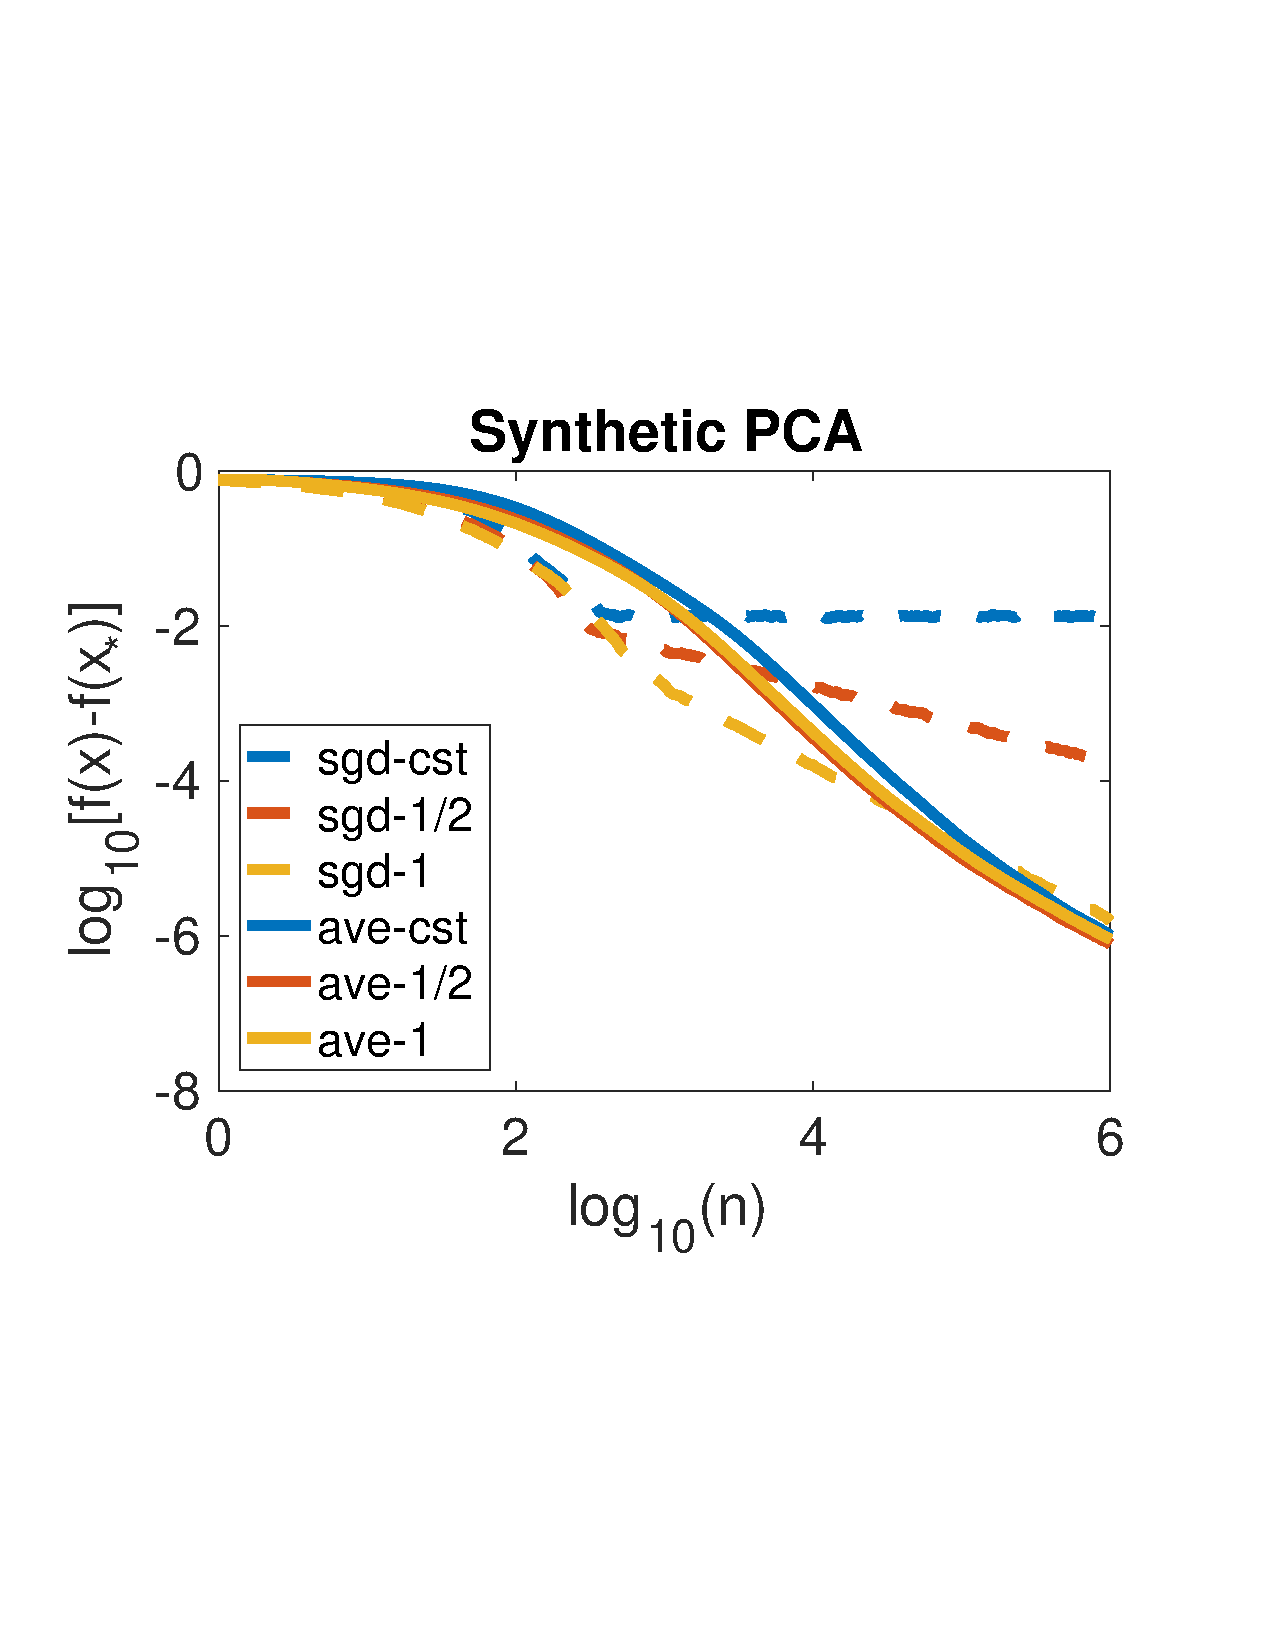
\includegraphics[width=\linewidth]{Figs/gapgrand}
   \end{minipage}
    \hspace*{-10pt}
   \begin{minipage}[c]{.45\linewidth}
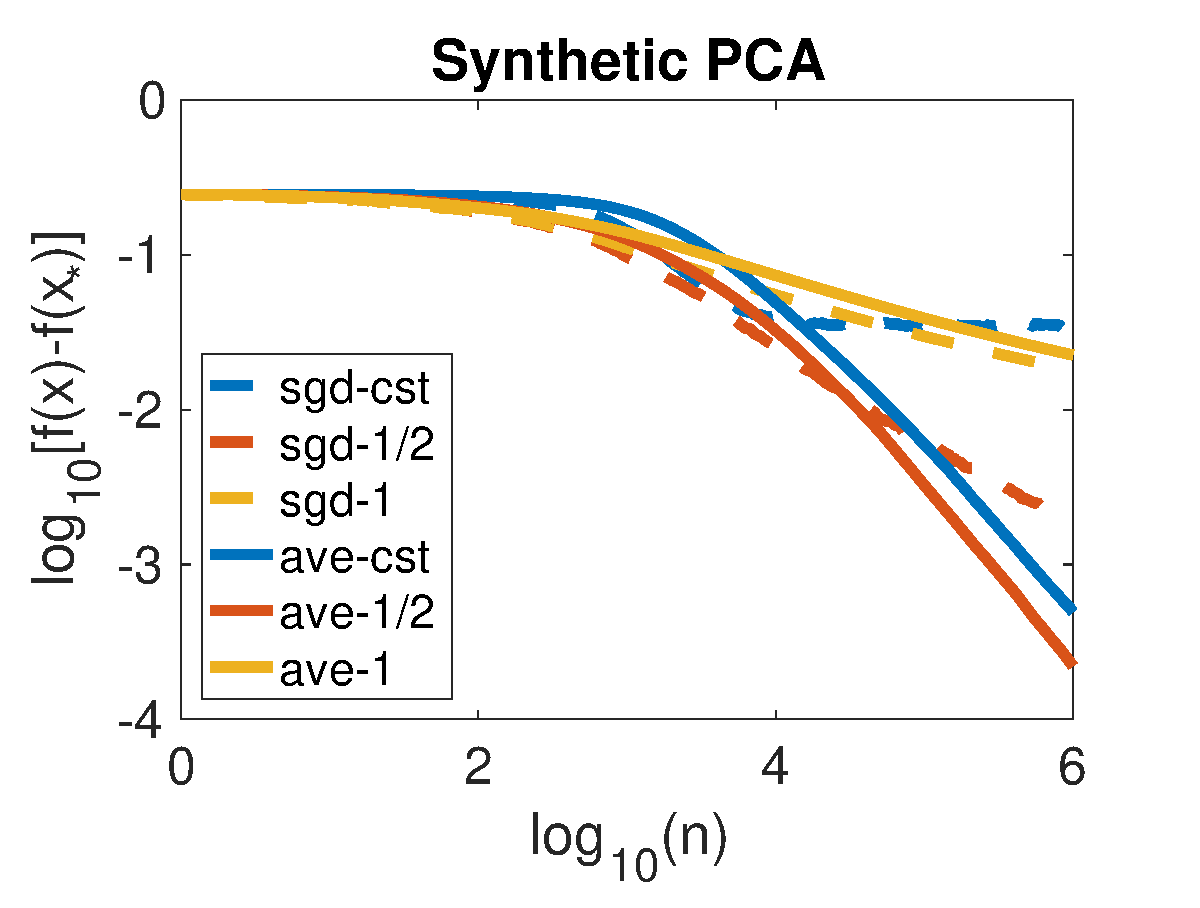
\includegraphics[width=\linewidth]{Figs/gappetit}
   \end{minipage}
   \vspace{-2.25cm}
  \caption{Streaming PCA. Left: Well-conditioned problem. Right: Poorly-conditioned problem.}
     \label{fig:synthetic}
  \vspace{-0.2cm}
\end{figure}
\begin{theorem} \label{thm:oja_main}
  Let Assumption~\ref{assump:manifold} hold for the set $\X = \{ X : \Vert X_\star^\top X\Vert_F^2 \geq k-\eta \}$, for some constant $0 < \eta <\frac{1}{4}$, where $X_\star$ minimizes $f(X)$ over the $k$-Grassmann manifold. Denote, $\tilde{H}_n =  H^{-1/2} H_n H^{-1/2}$, and the 4th-order tensor $C_{ii'jj'} = \E [(v_i^\top \tilde H_n v_j) (v_{i'}^\top \tilde H_n v_{j'})]$. Further assume that $\norm{H_n}_2 \leq 1$ a.s., and that $\lambda_k > \lambda_{k+1}$. Then if $X_n$ and $\tilde{X}_n$ evolve according to \eq{robust_oja}, there exists a positive-definite matrix $C$, such that $\tilde{\Delta}_n = R_{X_{\star}}^{-1}(\tilde{X}_n)$ satisfies:
  \vspace*{-6pt}
  \begin{align}
   \sqrt{n} \tilde{\Delta}_n \overset{D}{\to}  \mathcal{N}(0, C) \ \ \text{ with } \ \     C = \sum_{j'=1}^k\sum_{i'=k+1}^d \sum_{j=1}^k\sum_{i=k+1}^d C_{ii'jj'} \frac{\sqrt{\lambda_i \lambda_j} \cdot \sqrt{\lambda_{i'} \lambda_{j'}}}{(\lambda_{j}-\lambda_{i}) \cdot (\lambda_{j'}-\lambda_{i'})} (v_i e_j^\top) \otimes (v_{i'} e_{j'}^\top). \notag
  \end{align}
\end{theorem}
We  make the following observations:
\begin{itemize}
\vspace*{-6pt}
  \item If the 4th-order tensor satisfies\footnote{For example if $H_n = h_n h_n^\top$ for $h_n \sim \mathcal{N}(0, \Sigma)$ -- so $H_n$ is a rank-one stream of Gaussian random vectors -- this condition is satisfied. See the proof of Theorem \ref{thm:oja_main} for more details.} $C_{ii'jj'} = \kappa \delta_{ii'}\delta_{jj'}$ for constant $\kappa$, the aforementioned covariance structure simplifies to 
$
    C = \kappa \sum_{j=1}^k\sum_{i=k+1}^d\frac{{\lambda_i \lambda_j}}{(\lambda_j-\lambda_i)^2} (v_i e_j^\top) \otimes (v_{i} e_{j}^\top)
    $.
  This asymptotic variance matches the result
  of \citet{reiss2016non}, achieving the same statistical performance as the empirical risk minimizer and matching the lower bound
  of \citet{CaiMaWu13} obtained for the (Gaussian) spiked covariance model. 
  \vspace*{-6pt}
  \item Empirically, even using a constant step size in \eq{robust_oja} appears to yield convergence in a variety of situations; however, we can see a numerical counterexample in \myapp{counter}. We leave it as an open problem to understand the convergence of the iterate-averaged, constant step-size algorithm in the case of Gaussian noise \citep{BouLac85}.
  \vspace*{-6pt}
 \item Assumption~\ref{assump:manifold} could be relaxed using a martingale concentration result showing the iterates $X_n$ are restricted to $\X$ with high probability similar to the work of \citet{shamir16b} and \citet{AllenLi2017-streampca}.
 \vspace*{-4pt}
\end{itemize}
Note that we could also derive an analogous result to Theorem \ref{thm:oja_main} for the (averaged) Riemannian SGD algorithm in \eq{grad_desc} and \eq{ave_grad_desc}. However, we prefer to present the algorithm in \eq{robust_oja} since it is simpler and directly averages the (commonly used) randomized power method.

% !TEX root = main.tex
\newpage
\section{Experiments} \label{sec:experiments}
\subsection{Image Classification}

Training a binary classifier with imbalanced data is a challenging task in machine learning. Practices for dealing with imbalance include optimizing class weight hyperparameters, hard negative mining \citep{shrivastava2016training} and synthetic minority oversampling \citep{chawla2002smote}. 
Without accounting for imbalance, the minority samples are often misclassified in early stages of the iterative training procedures, resulting in high loss and high gradient norms associated with these points. Importance sampling schemes for reducing the variance of the gradient norms will sample these instances more often at the early phases, offering a way of tackling imbalance.

For verifying this intuition, we perform the image classification experiment of \cite{bouchard2015online}. We train one-vs-all logistic regression Pascal VOC 2007 dataset \citep{everingham2010pascal} with image features extracted from the last layer of the VGG16 \citep{simonyan2014very} pretrained on Imagenet. We measure the average precision by reporting its mean over the 20 classes of the test data. The optimization is performed with AdaGrad \citep{duchi2011adaptive}, where learning rate is initialized to 0.1. The losses received by the bandit methods are the norms of the logistic loss gradient.
We compare our method, Variance Reducer Bandit (VRB), to:
\vspace{-1.5mm}
\begin{itemize}
\setlength\itemsep{0.05em}
\item uniform sampling for SGD,
\item Adaptive Weighted SGD (AW) \citep{bouchard2015online} ---  variance reduction by sampling from a chosen distribution whose parameters are optimized alternatingly with the model parameters,
\item MABS \citep{salehi2017} --- bandit algorithm for variance reduction that relies on EXP3 through employing modifies losses.  
\end{itemize}

\begin{figure}[h]
\centering
\begin{minipage}{.48\textwidth}
  \centering
  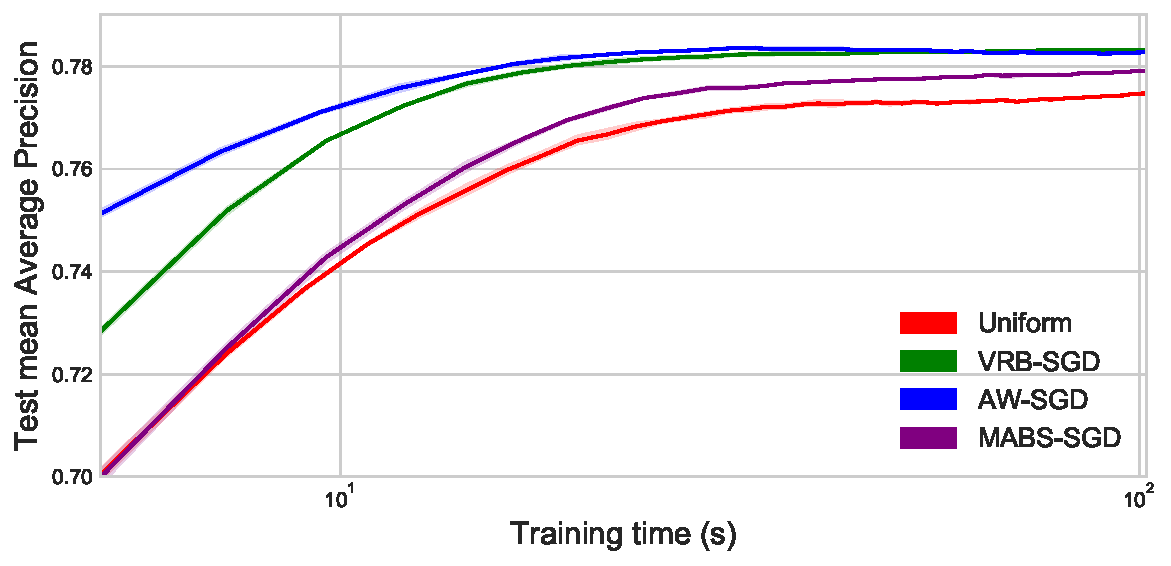
\includegraphics[width=\linewidth]{figures/voc-result.pdf}
      \caption{Mean Average Precisions on the test part of VOC 2007.}
      \label{fig:voc-results}
\end{minipage}%
\quad
\begin{minipage}{.48\textwidth}
  \centering
  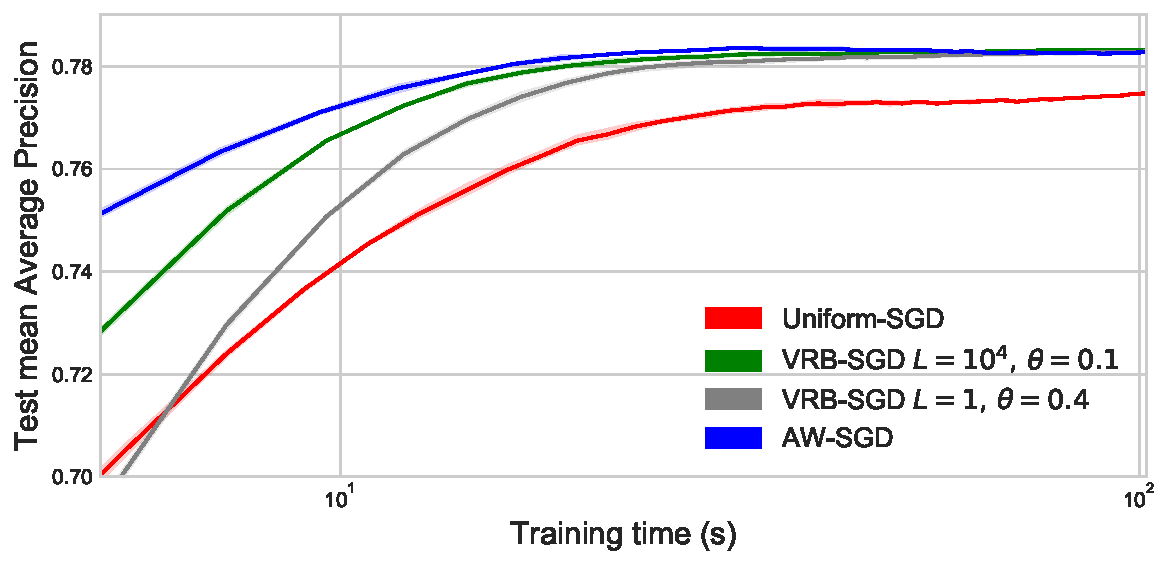
\includegraphics[width=\linewidth]{figures/voc-result-2.pdf}
      \caption{The effect of different hyperparameters on VRB. }
      \label{fig:voc-results-2}
\label{fig:test}
\end{minipage}%
\end{figure}

        
The hyperparameters of the methods are chosen based on cross-validation on the validation portion of the dataset. The results can be seen in Figure \ref{fig:voc-results}, where the shaded areas represent confidence $95\%$ intervals over 10 runs. The best performing method is AW, but its disadvantage compared to the bandit algorithms is that it requires choosing a family of sampling distributions, which usually incorporates prior knowledge, and calculating the derivative of the log-density. VRB and AW both outperform uniform subsampling with respect to the training time.  VRB performs similarly to AW at convergence, and speeds up training 10 times compared to uniform sampling, by attaining a certain score level 10 times faster. We have also experimented with the variance reduction method of \cite{pmlr-v70-namkoong17a}, but it did not outperform uniform sampling significantly. Since cross-validation is costly, in Figure \ref{fig:voc-results-2} we show the effect of the hyperparameters of our method. More specifically, we compare the performance of VRB with misspecified regularizer $L=1$ to the best $L=10^8$ chosen by cross-validation, and we compensate by using higher mixing coefficient $\theta=0.4$. The fact that only the early-stage performance is affected is a sign of method's robustness against regularizer misspecification.

We also measure the regret incurred both by the full information and VRB samplers, and show the results in Figure \ref{fig:regret}. For a fair comparison, we choose an \emph{oblivious} adversary that generates the loss sequences by performing the same optimization process as described above on a subset of 1000 data points from VOC 2007, with uniform sampling. For VRB, we report the average regret over 10 runs. 
\begin{figure}[h]

		\centering
		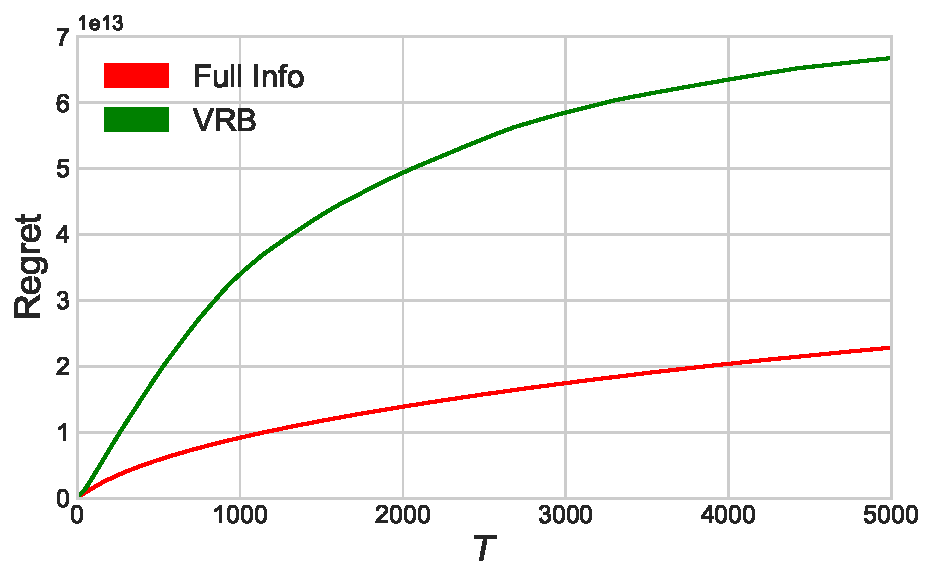
\includegraphics[width=0.5\linewidth]{figures/regret.pdf}
		\caption{Regret incurred by the full info and VRB.}
		\label{fig:regret}
\end{figure}


\subsection{$k$-Means}

In this experiment, we show that in some applications it is beneficial to work with per-sample upper bound estimates $L_i$ instead of a single global bound. As an illustrative example, we choose mini-batch $k$-Means clustering \citep{sculley2010web}. This is a slight deviation from the presented theory, since we sample multiple points for the batch and update the sampler only  once, upon observing the loss for the batch. 

In the case of $k$-Means, the parameters consist of the coordinates of the $k$ centers \linebreak $Q=\{q_1, q_2, \dots, q_k\}$. As the cost function for a point $x_i \in \{x_1, x_2, \dots, x_n \}$ is the  squared Euclidean distance to the closest center, the loss received by VRB  is the norm of the gradient  \linebreak $\min _{q \in Q } 2 \cdot || x_i - q||_2$. This lends itself to a natural estimation of $L_i$:
choose a point $u$ randomly from the dataset and define $L_i=4 \cdot || x_i - u||^2_2$. For this experiment, we set $\theta=0.5$.

We solve mini-batch $k$-Means  for $k=100$ and batch size $b=100$ with uniform sampling and VRB. The initial centers are chosen with $k$-Means++ \citep{arthur2007k} from a random subsample of 1000 points from the training data and they are shared between the methods. We generate 10 different sets of initial centers and run both algorithms 10 times on each set of centers, with different random seeds for the samplers.  We train the algorithm on $80 \%$ of the data, and measure the cost of the $20 \%$ test portion for the following datasets:
\vspace{-2mm}
\begin{itemize}
\setlength\itemsep{0.2em}
  \item \texttt{CSN} \citep{faulkner2011next} --- cellphone accelerometer with 80,000 observations and 17 features,
 \item \texttt{KDD} \citep{kddcup2004} --- data set used for Protein Homology Prediction KDD
    competition  containing 145,751 observations with 74 features,
    \item \texttt{MNIST} \citep{lecun1998gradient} --- 70,000 low resolution images of handwritten
    characters transformed using PCA with whitening and retaining 10 dimensions.  
\end{itemize}

\begin{figure}[h]
      \centering
      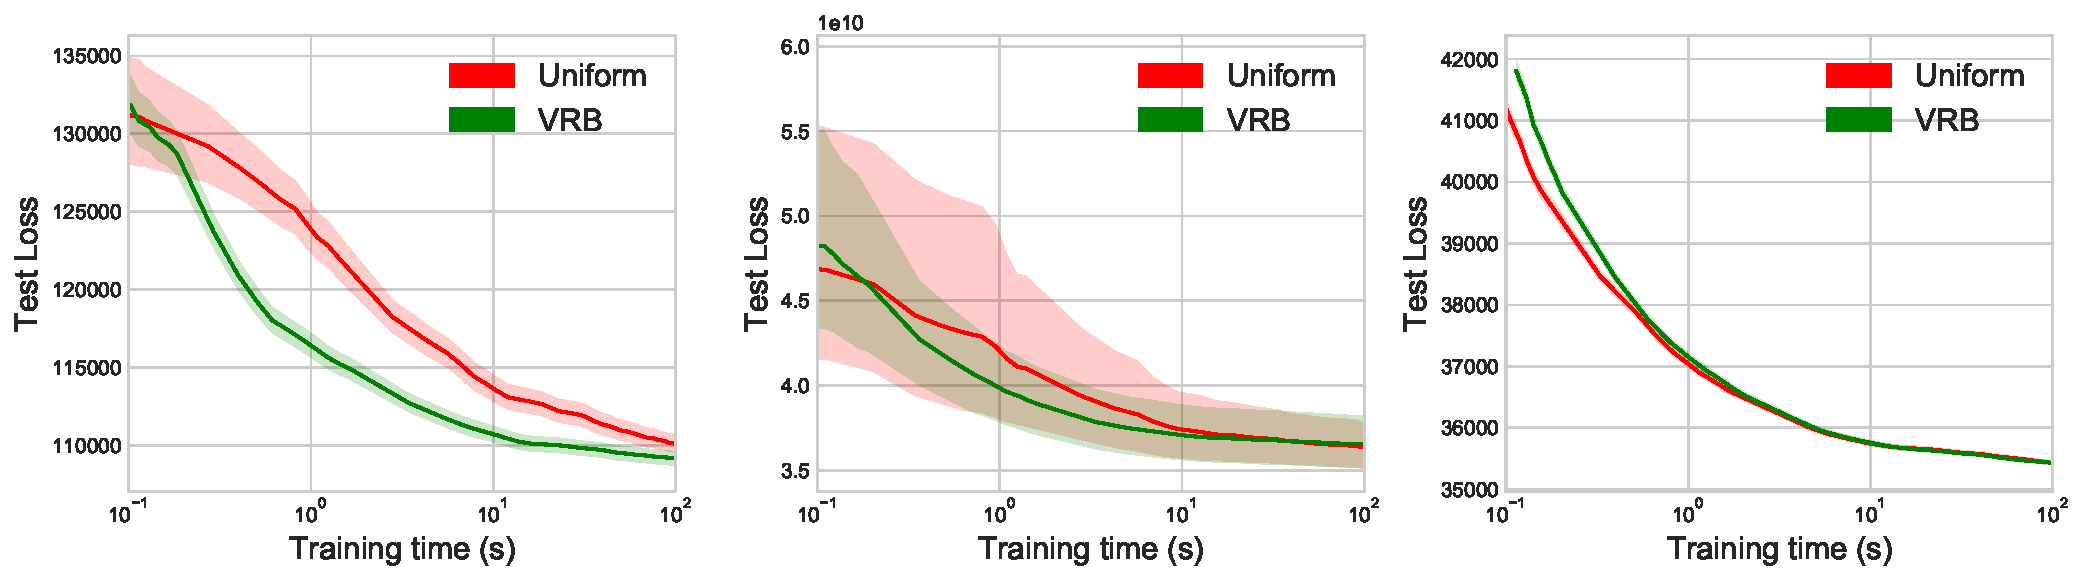
\includegraphics[width=\linewidth]{figures/kmeans.pdf}
      \caption{The evolution of the loss of $k$-Means on the test set. The shaded areas represent $95\%$ confidence intervals over 100 runs.}
      \label{fig:kmeans-results}
        \end{figure}
        
The evolution of the cost function on the test set with respect to the elapsed training time is shown in Figure \ref{fig:kmeans-results}. The chosen datasets illustrate three observed behaviors of our algorithm. In the case of \texttt{CSN}, our method significantly outperforms uniform subsampling. In the case of \texttt{KDD}, the advantage of our method can be seen in the reduced variance of the cost over multiple runs, whereas on \texttt{MNIST} we observe no advantage.
This behavior is highly dependent on intrinsic dataset characteristics: for \texttt{MNIST}, we note that the entropy of the best-in-hindsight sampling distribution is close the entropy of the uniform distribution. We have also compared VRB with the bandit algorithms mentioned in the previous section. Since mini-batch $k$-Means converges in 1-2 epochs, these methods with  uniform initialization do not outperform uniform subsampling significantly. Thus, for this setting, careful initialization is necessary, which is naturally supported by our method.

% !TEX root = main.tex

\section{Conclusions}

In this paper, we showed that even though non-convex approaches for matrix completion are not robust in the semi-random model, but it is possible to fix them using a pre-processing step.
The pre-processing step solves a few convex programs (packing SDPs) to ameliorate the influence of the semi-random adversary. %, and produces a weighted instance with spectral properties similar to a random graph.
Unlike the full convex relaxation for matrix completion, our pre-processing step runs in nearly-linear time. Combining our pre-processing step with non-convex optimization gives an algorithm that is robust in the semi-random model, and at the same time enjoys the efficiency of the non-convex approaches.

%Our pre-processing step solves a variant of the graph sparsification problem.
%Given a graph $G$ formed by adding extra edges to $H$ (or a graph similar to $H$), we can produce a weighted version of $G$ that is spectrally similar to $H$.
%We believe this subroutine can be useful in other problems.

An immediate open problem is whether we can prove the output of the pre-processing step allows non-convex optimization to recover the ground truth {\em exactly}.
%This would require proving stronger concentration inequalities like Lemma~\ref{lem:tangent} using deterministic conditions.
More broadly, we hope this work will inspire new ideas that make non-convex optimization more robust.

%\newpage
\bibliographystyle{plainnat}
\bibliography{onlinepca}

\newpage
\onecolumn
\appendix
%!TEX root = main.tex
\section{Appendices}

In \myapp{main_proof} we provide the proof of Theorem \ref{thm:main}. In \myapp{app_pfsketch} we prove the relevant lemmas mirroring the proof sketch in \mysec{pfsketch}. In \myapp{appapp} we provide proofs of the results for the application discussed in \mysec{geostrong} about geodesically-strongly-convex optimization. \mysec{stream_pca_app} contains background and proofs of results discussed in \mysec{stream_pca} regarding streaming $k$-PCA. \mysec{counter} contains further experiments on synthetic PCA showing a counterexample to the convergence of averaged, constant step-size SGD mentioned in \mysec{experiments} in the main text.

Throughout this section we will denote a sequence of vectors $X_{n}$ to be $X_{n} = O(f_n)$, for scalar functions $f_n$,
if there exists a constant $C>0$, such that $\norm{X_{n+1}} \leq C f_n$ for all $n \geq 0$ almost surely.
\section{Proofs for \mysec{results}} \label{sec:main_proof}
Here we provide the proof of Theorem \ref{thm:main}. The first statement follows by combining Theorems \ref{thm:linear}, \ref{thm:asymp_ave}, Lemma \ref{lem:stream_avg_iters} and Slutsky's theorem. The second statement follows by using Theorems \ref{thm:linear}, \ref{thm:nonasymp_ave}, and Lemma \ref{lem:stream_avg_iters_4mom}.

\section{Proofs for \mysec{pfsketch}} \label{sec:app_pfsketch}
Here we detail the proofs results necessary to conclude our main result sketched in
\mysec{pfsketch}.

\subsection{Proofs in \mysec{pfsketch1}}
We begin with the proofs of the geometric lemmas detailed in \mysec{pfsketch1},
showing how to linearize the progress of the SGD iterates $x_n$ in the tangent space of $x_\star$ by considering the evolution of $\Delta_n = R_{x_\star}^{-1}(x_n)$. Note that since by Assumption~\ref{assump:manifold}, for all $n\geq0$, $x_n\in\X$, the vectors $\Delta_n$ all belong to the compact set $R_{x_\star}^{-1}(\X)$.

% Moreover considering iterates restricted to a compact $\X$, using Assumption~\ref{assump:manifold}, no global conditions on curvature are necessary for Theorem \ref{thm:main}, since as smooth function restricted to $\X$ they will be bounded.

In the course of our argument it will be useful to consider the function $F_{x, y}(\eta_x) = R_y^{-1} \circ R_x(\eta_x) : T_x \M \to T_x \M$
 (which crucially
is a function defined on a vector space) and further $D R_x(\eta_x) : T_x \M \to T_{R_x(\eta_x)} \M$, the linearization of the retraction map. The first recursion we will study is that of $\Delta_{n+1} = F_{x_n, x_\star}(-\gamma_{n+1} \nabla f_{n+1}(x_n))$:
\begin{lemma}\label{lem:tangent_rec}
Let Assumption \ref{assump:manifold} hold. If $\Delta_n = R_{x_\star}^{-1}(x_n)$ for a sequence of iterates evolving as in  \eq{grad_desc}, then there exists a constant $C_{\text{manifold}}>0$ depending on $\X$ such that,
  \[
  \D_{n+1} = \D_n - \gamma_{n+1} [\te{x_\star}{x_n}]^{-1} (\nabla f_{n+1}(x_n)) + \gamma_{n+1} g_n,
  \]  where $\norm{g_n} \leq \gamma_{n+1} C_{\text{manifold}} \norm{\nabla f_{n+1}(x_n)}^2$.
\end{lemma}
\begin{proof}
  Using the chain rule for the differential of a mapping on a manifold and the first-order property of the retraction ($D R_x (0_x) = \idm_{T_x\M}$)
  we have that:
  \begin{multline*}
      D F_{x, y}(0_x) = D(R_y^{-1} \circ R_x)(0_x) = D R_{y}^{-1}(R_x(0_x)) \circ D R_x(0_x) \\= [D R_y(R_{y}^{-1}(R_x(0_x)))]^{-1} \circ \idm_{T_x \M} =    [DR_y(R_{y}^{-1}(x))]^{-1}=[\te{y}{x}]^{-1},
  \end{multline*}
  where the last line follows by the inverse function theorem on the manifold $\M$.
 Smoothness of the retraction  implies the Hessian of $F_{x, y}$ is uniformly bounded in norm on the compact set $F_{x, y}^{-1}(R_{x_\star}^{-1}(\X))$. We use $C_{\text{manifold}}$ to denote a bound on the operator norm of the Hessian of $F_{x, y}$ in this compact set. In the present situation,
  we have that $\Delta_{n+1} = F_{x_n, x_\star}(-\gamma_{n+1} \nabla f_{n+1}(x_n))$. Since $F_{x_n, x_\star}$ is a function defined on vector spaces the result follows using a Taylor expansion,
  $F_{x_n, x_\star}(0)=\Delta_n$, the previous statements regarding the differential of $F_{x_n, x_\star}$, and the uniform bounds on the second-order terms. In particular, the second-order term in the Taylor expansion is upper bounded as $\gamma_{n+1} C_{\text{manifold}} \norm{\nabla f_{n+1}(x_n)}^2$ so the bound on the error term $g_n$ follows.
\end{proof}
We now further develop this recursion by also considering an asymptotic expansion of the gradient term near the optima.
\begin{lemma}\label{lem:tangent_rec_2}
Let Assumptions \ref{assump:HessianLip}, \ref{assump:noiseunbiased},  and \ref{assump:noiseLip} hold.
If $\Delta_n = R_{x_{\star}}^{-1}(x_n)$ for a sequence of iterates evolving as in \eq{grad_desc},  then there exist sequences $\{ \tilde \xi_n \}_{n \geq 0}$ and $\{ \tilde e_n \}_{n \geq 0}$ such that
  \[
 \tp{x_n}{x_\star} \nabla f_{n+1}(x_n)=\Hess f(x_\star)\Delta_n + \nabla f_{n+1}(x_\star)+\tilde \xi_{n+1}+\tilde e_{n+1},
  \]
where $\E[\ \tilde \xi_{n+1}\vert\mathcal F_{n}]=0$, $\E[\Vert \tilde\xi_{n+1}\Vert^2 \vert\mathcal F_{n}]\leq 4 L \Vert \Delta_n\Vert^2$ and $\tilde e_{n+1}$ such that $\Vert\tilde e_{n+1}\Vert \leq \frac{M}{2}\Vert \Delta_n\Vert^2$.
\end{lemma}
\begin{proof}
We begin with the decomposition:
\BEAS
\Hess \!\! f(x_\star)\Delta_n&\!\!\!=\!\!\!& \tp{x_n}{x_\star} \nabla f(x_n) - \nabla f(x_\star) +[\Hess \!\!f(x_\star)\Delta_n-\tp{x_n}{x_\star} \nabla f(x_n) - \nabla f(x_\star) ] \\
&\!\!\!=\!\!\!&  \tp{x_n}{x_\star}\!\! \nabla f_{n+1}(x_n) - \nabla f_{n+1}(x_\star) +[\Hess \!\!f(x_\star)\Delta_n-\tp{x_n}{x_\star} \!\!\nabla f(x_n) \!-\! \nabla f(x_\star) ] \\
&&+  [\tp{x_n}{x_\star} \nabla f(x_n) - \nabla f(x_\star) - \tp{x_n}{x_\star} \nabla f_{n+1}(x_n) + \nabla f_{n+1}(x_\star)].
\EEAS
Under Assumption \ref{assump:HessianLip}, using the manifold version of Taylor's theorem (see \citet{absil2009optimization} Lemma 7.4.8) we have for $\tilde e_{n+1}=   \Hess f(x_\star) \Delta_n -\tp{x_n}{x_{\star}} \nabla f(x_n)$, that
\[
\Vert \tilde e_{n+1}\Vert \leq \frac{M}{2}\Vert \D_n\Vert^2.
\]
Denoting $\tilde \xi_{n+1}=  [\tp{x_n}{x_\star} \nabla f(x_n) - \nabla f(x_\star) - \tp{x_n}{x_\star} \nabla f_{n+1}(x_n) + \nabla f_{n+1}(x_\star)]$, Assumption \ref{assump:noiseunbiased} directly implies that $\E[\ \tilde \xi_{n+1}\vert\mathcal F_{n}]=0$. Finally, using Assumption \ref{assump:noiseLip} and the elementary inequality $2 \E[A \cdot B | \F_n] \leq \E[A^2 | \F_n] + \E[B^2 | \F_n]$ for square-integrable random variables $A, B$ shows that,
\BEAS
\E[\Vert \tilde\xi_{n+1}\Vert^2 \vert\mathcal F_{n}]
&\leq& 2\Vert \tp{x_n}{x_\star} \nabla f(x_n) - \nabla f(x_\star) \Vert^2 + 2 \E \left[\Vert \tp{x_n}{x_\star} \nabla f_{n+1}(x_n) - \nabla f_{n+1}(x_\star) \Vert^2 | \F_n \right] \\
&\leq &4L^2 \Vert \D_n \Vert^2.
\EEAS
\end{proof}
The last important step to conclude a linear recursion in $\Delta_n$ is to argue that the operator composition
$ [\te{x_\star}{x_n}]^{-1}\tp{x_\star}{x_n} : T_{x_\star}\M \to  T_{x_\star}\M$, is in fact an
isometry (up to 2nd-order terms) since $x_n$ is close to $x_\star$. The following argument crucially uses the fact that $R_{x_\star}$ is a second-order retraction.
\begin{lemma} \label{lem:tangent_rec_3}
 Let Assumption \ref{assump:manifold}. Let $\Delta_n = R_{x_{\star}}^{-1}(x_n)$ for a sequence  $\{ x_n \}_{n \geq 0}$ evolving as in \eq{grad_desc}. Then there exists a trilinear operator $K(\cdot,\cdot,\cdot)$ such that
  \[
    [\te{x_\star}{x_n}]^{-1}\tp{x_\star}{x_n} = I - K(\Delta_n,\Delta_n, \cdot)   + O(\norm{\Delta_n}^3).
  \]
\end{lemma}
As noted in the proof, when the exponential map is used as the retraction, the operator $K$ is precisely the Riemann curvature tensor $R_{x_\star}(\D_n, \cdot)\D_n$ (up to a constant prefactor).
\begin{proof}
  We derive a Taylor expansion for the operator composition $[\tp{x}{y}]^{-1}\te{x}{y}$ when $y$ is close to $x$. Consider the function $G(v)= [\tp{x}{R_x(v)}]^{-1}\te{x}{R_x(v)}: T_x\M\to L(T_x\M)$ where $L(T_x\M)$ denotes the set of linear maps on the vector space $T_x\M$. Now, recall that $\tp{x}{R_x(tv)}$ is precisely the parallel translation operator along the curve $\gamma(t)=R_y(tv)$. From Proposition 8.1.2 by \citet{absil2009optimization}, we have that
  \[
  \frac{d}{dt} G(tv)\vert_{t=0} =   \frac{d}{dt}  [\tp{x}{R_x(tv)}]^{-1}\te{x}{R_x(tv)}\vert_{t=0} = \nabla_{\dot \gamma(0)} D R_y,
  \]
  where $\nabla$ denotes the Levi-Civita connection (see also the proof of \citet[Lemma 7.4.7]{absil2009optimization} and \citet[Chapter 2, Exercise 2]{do2016differential}). Using the definition of the covariant derivative $\nabla_{v}$ along a vector $v$, and of the acceleration vector field $\dot{\gamma}$ \citep[Section 5.4]{absil2009optimization}
  we have that
  \[
   \nabla_{\dot \gamma(0)} D R_y= \frac{D}{dt} D R_y(\gamma(t))\vert_{t=0} = \frac{D^2}{dt^2} R_y(tv)\vert_{t=0}=0,
  \]
  since $R$ is a second-order retraction. Thus, $  \frac{d}{dt} G(tv)\vert_{t=0}=0$.

 We use $K$ to denote the symmetric trilinear map $d^2G(0)$, where $K(v,v,\cdot)=\frac{1}{2}\frac{d^2}{dt^2} G(tv)\vert_{t=0}$. Thus, since $G$ is smooth and the iterates are restricted to $\X$ by Assumption \ref{assump:manifold},
 a Taylor expansion gives, for $v\in R_{x_\star}^{-1}(\X)$,
 $
 G(v)=G(0)+K(v,v,\cdot)+O(\Vert v \Vert^3)
 $.
 For $x=x_\star$ and $v=\Delta_n$, this yields
 \[
 [\tp{x_\star}{x_n}]^{-1}\te{x_\star}{x_n}= I+K(\Delta_n,\Delta_n,\cdot)+O(\Vert \D_n \Vert^3).
 \]
 Lastly, as
  $  [\te{x_\star}{x_n}]^{-1}\tp{x_\star}{x_n} = \left([\tp{x_\star}{x_n}]^{-1} \te{x_\star}{x_n} \right)^{-1} = \left( I + K(\Delta_n,\D_n, \cdot) + O(\norm{\Delta_n}^3)) \right)^{-1} = I -  K(\Delta_n, \D_n,\cdot)  + O(\norm{\Delta_n}^3)$
  the conclusion follows.
In the special case the exponential map is used as retraction, \citet[][Theorem A.2.9]{waldmann2012geometric}  directly relates $K$ to the Riemann curvature tensor. They show $K(v,v,\cdot)=-\frac{1}{6}R_{x_\star}(v,\cdot)v$ for $v\in T_{x_\star}\M$. However the result by \citet{waldmann2012geometric} provides the Taylor expansion up to arbitary order in $\Vert v \Vert$.
\end{proof}
Assembling Lemmas  \ref{lem:tangent_rec}, \ref{lem:tangent_rec_2} and \ref{lem:tangent_rec_3} we obtain the desired linear recursion:
\begin{theorem}\label{thm:linear}
  Let Assumptions \ref{assump:manifold}, \ref{assump:HessianLip}, \ref{assump:noiseunbiased},  and \ref{assump:noiseLip} hold. If $\Delta_n = R_{x_{\star}}^{-1}(x_n)$ for a sequence of iterates evolving as in \eq{grad_desc}, then there exists a martingale-difference sequence $\{ \xi_{n} \}_{n \geq 0}$ satisfying  $\E[\xi_{n+1}\vert \F_{n}]=0$,
$ \E[\Vert \xi_{n+1}\Vert^2 \vert \F_{n}] = O(\norm{\D_n}^2) $, and an error sequence $\{ e_n \}_{n \geq 0}$ satisfying $\mathbb{E}[ \norm{ e_{n+1} } | \F_{n} ] \Vert = O(\norm{\Delta_n}^2 + \gamma_{n+1})$ and
$\mathbb{E}[ \norm{ e_{n+1} }^2 | \F_n ] \Vert = O(\norm{\Delta_n}^4 + \gamma_{n+1}^2)$ such that
  \[
    \D_{n+1} = \D_n - \gamma_{n+1} \Hess f(x_\star) \Delta_n  -\gamma_{n+1} \nabla f_{n+1}(x_\star) \\ -\gamma_{n+1}\xi_{n+1}  -\gamma_{n+1} e_{n+1}.
  \]
\end{theorem}
\begin{proof} Combining Lemmas \ref{lem:tangent_rec},  \ref{lem:tangent_rec_2} and \ref{lem:tangent_rec_3},
\BEAS
  \D_{n+1} &=& \D_n - \gamma_{n+1} [\te{x_\star}{x_n}]^{-1} (\nabla f_{n+1}(x_n)) + \gamma_{n+1} g_n \\
   &=& \D_n - \gamma_{n+1} [\tp{x_n}{x_\star}\te{x_\star}{x_n}]^{-1} \tp{x_n}{x_\star}(\nabla f_{n+1}(x_n)) + \gamma_{n+1} g_n \\
   &=& \D_n - \gamma_{n+1} [I -  K(\Delta_n,\D_n, \cdot) ] \circ (\Hess f(x_\star)\Delta_n + \nabla f_{n+1}(x_\star)+\tilde\xi_{n+1}+\tilde e_{n+1}) \\
   && + \gamma_{n+1} g_n + O( \gamma_{n+1} \Vert \D_{n}\Vert^3)\\
   &=& \D_n - \gamma_{n+1} \Hess f(x_\star)\Delta_n  -\gamma_{n+1} \nabla f_{n+1}(x_\star)\\
   &&-\gamma_{n+1}\tilde \xi_{n+1}  +{\gamma_{n+1}} K(\Delta_n,\Delta_n,\nabla f_{n+1}(x_\star)+\tilde \xi_{n+1} ) \\
      &&-\gamma_{n+1}\tilde e_{n+1} +{\gamma_{n+1}} K(\Delta_n,\Delta_n,\Hess f(x_\star) \Delta_n +\tilde e_{n+1}) \\
      && + \gamma_{n+1} g_n + O( \gamma_{n+1} \Vert \D_{n}\Vert^3).
 \EEAS
 Let $\xi_{n+1} = \tilde \xi_{n+1}  -{\gamma_{n+1}} K(\Delta_n,\Delta_n,\nabla f_{n+1}(x_\star)+\tilde \xi_{n+1} )$. By linearity of the map $K(\D_n,\D_n,\cdot)$,  $\E[\xi_{n+1}\vert \F_{n}]=0$. Moreover by smoothness of the retraction, the tensor $K$ is uniformly bounded in injective norm on the compact set $R_{x_\star}^{-1}(\X)$, so $\E[\Vert \xi_{n+1}\Vert^2 \vert \F_{n}] = O(\Vert \D_n\Vert^2)$.

 Let $e_{n+1}=\tilde{e}_{n+1} - K(\Delta_n,\Delta_n,\nabla^2 f(x_\star)+\tilde{e}_{n+1} ) - g_{n} +O( \Vert \D_{n}\Vert^3)$. Using Assumptions \ref{assump:manifold}, \ref{assump:noiseLip} and the almost sure upper bound on $\tilde {e}_{n+1}$ we have that this term satisfies
 \[
 \E[\Vert e_{n+1}\Vert ^2 | \F_n] = \O \left(\norm{\Delta_n}^4 + \gamma_{n+1}^2 \right).
 \]
\end{proof}
Note that sharper bounds may be obtained under higher-order assumptions on the moments of the noise.  This would provide a sharp constant of the leading asymptotic term of $O(\frac{1}{n})$, when the step-size $\gamma_n=\frac{1}{\sqrt{n}}$ is used.

%!TEX root = main.tex
\subsection{Proofs in \mysec{pfsketch2}} \label{sec:conv_rates}
Here we provide proofs, in the Euclidean setting, of both asymptotic and non-asymptotic Polyak-Ruppert-type averaging results. We apply these results to the tangent vectors $\Delta \in T_{x_\star}\M$ as described in \mysec{pfsketch1}.
\subsubsection{Asymptotic Convergence}
Throughout this section, we will consider a general linear recursion perturbed by a remainder term $e_n$ of the form:
\begin{align}
  \D_{n}=\D_{n-1} -\gamma_n A \D_{n-1}+ \gamma_n (\eps_n+\xi_{n}+e_{n}), \label{eq:rec_with_error1}
\end{align}
for which we will show an asymptotic convergence result under appropriate conditions.  

Note that we eventually apply these convergence results to iterates $\Delta_n \in T_{x_\star} \M$, which is a finite-dimensional vector space. In this setting, a probability measure can be defined on a vector space (with inner product) with a covariance operator implicitly depending on the inner product (via the dual map). 

We make the following assumptions on the structure of the recursion:
\begin{assumption} \label{assump:psd}
  $A$ is symmetric positive-definite matrix.
\end{assumption}
\begin{assumption} \label{assump:noise1}
    The noise process $\{ \eps_{n} \}$ is a martingale-difference process (with  $\E[\eps_n\vert\mathcal F_{n-1}]=0$  and  $\sup_n \E[\eps_n^2] < \infty$), for which    there exists $C>0$ such that $\E [\Vert \eps_n \Vert^4 | \mathcal{F}_{n-1}] \leq C$ for all $n \geq 0$ and a matrix $\Sigma \succ 0$ such that
    \[\E[\eps_n\eps_n^\top\vert\mathcal F_{n-1}]\overset{P}{\to} \Sigma.\]
\end{assumption}
\begin{assumption} \label{assump:noise2}
    The noise process $\{ \xi_{n} \}$ is a martingale-difference process (with  $\E[\xi_n\vert\mathcal F_{n-1}]=0$ and $\sup_n \E[\xi_n^2] < \infty$), and for sufficiently large $n \geq N$, there exists $K > 0$ such that
    \[ \E[\Vert \xi_n\Vert^2\vert\mathcal F_{n-1}] \leq K\gamma_n \text{ a.s. } \]
    with $\gamma_n \to 0$ as $n \to \infty$.
\end{assumption}
\begin{assumption} \label{assump:remainder}
  For $n \geq 0$
    \[
    \E[\Vert e_n \Vert] = O(\gamma_n).
    \]
\end{assumption}
\begin{assumption}\label{assump:step_size}
  $\gamma_n \to 0$, $\frac{\gamma_n-\gamma_{n-1}}{\gamma_n} = o(\gamma_n)$ and $\sum_{j=1}^{\infty} \frac{\gamma_j}{\sqrt{j}} < \infty$.
\end{assumption}
The first two conditions in Assumption \ref{assump:step_size} require that $\gamma_n$ decrease sufficiently slowly. For example $\gamma_n = \gamma t^{-\alpha}$ with $ \frac{1}{2} < \alpha < 1$ satisfy these two conditions
but the sequence $\gamma = \gamma t^{-1}$ does not.

We can now derive the asymptotic convergence rate,
\begin{theorem} \label{thm:asymp_ave}
  Let Assumptions \ref{assump:psd}, \ref{assump:noise1}, \ref{assump:noise2}, \ref{assump:remainder} and \ref{assump:step_size}
  hold for the perturbed linear recursion in Equation \eqref{eq:rec_with_error1}.
  Then,
\[
\sqrt n \bar{\Delta}_n  \overset{D}{\to} \mathcal N (0,  A^{-1}\Sigma A^{-1}).
\]
\end{theorem}
\begin{proof}
The argument mirrors the proof of Theorem 2 in \citet{polyak1992acceleration} so we only
sketch the primary points. Throughout we will use $C$ to denote an unimportant, global constant that may change line to line.

Consider the purely linear recursion of the form:
\begin{align}
  & \D^1_{n}=\D^1_{n-1} -\gamma_n A \D^1_{n-1}+ \gamma_n (\eps_n+\xi_{n}) \label{eq:linear_rec} \\
  & \bar{\D}^1_{n} = \frac{1}{n} \sum_{i=0}^{n-1} \D^1_{i}, \nonumber
\end{align}
which satisfies $\D^1_{0} = \D_{0}$, and approximates the perturbed recursion in Equation \eqref{eq:rec_with_error1},
\begin{align}
  & \D_{n}=\D_{n-1} -\gamma_n A \D_{n-1}+ \gamma_n (\eps_n+\xi_{n}) + \gamma_n e_{n} \label{eq:linear_rec_perturb} \\
  & \bar{\D}_{n} = \frac{1}{n} \sum_{i=0}^{n-1} \D_{i}. \nonumber
\end{align}
Now, note that we can show that
$\lim_{K \to \infty} \lim \sup_{n} \E \left[\Vert \eps_n \Vert^2 \mathbb{I}[\Vert \eps_n \Vert > K]|\F_{n-1} \right] \overset{p}{\to} 0$, using our (conditional) 4th-moment bound and the (conditional) Cauchy-Schwarz/Markov inequalities, so the relevant assumption in \citet{polyak1992acceleration} is satisfied. Then as the argument in Part 3 of the proof of Theorem 2 in
\citet{polyak1992acceleration} shows, under Assumptions \ref{assump:psd}, \ref{assump:noise1}, \ref{assump:noise2}
the conditions of Proposition (a) of Theorem 1 in \citet{polyak1992acceleration} also hold. This implies the linear process
satisfies:
\[
\sqrt n \bar{\D}^1_n  \overset{D}{\to} \mathcal N (0,  A^{-1}\Sigma A^{-1}). \notag
\]
We now argue that the process $\bar{\D}^1_n$ and $\bar{\D}_n$ are asymptotically equivalent in distribution. First,
since the noise process is coupled between Equations \ref{eq:linear_rec} and \ref{eq:linear_rec_perturb}, the differenced process
obeys a simple (perturbed) linear recursion,
\[
  \D_n - \D^1_{n} = (I-\gamma_j A)(\D_{n-1}-\D^1_{n-1}) - \gamma_n e_n. \notag
\]
Expanding and averaging this recursion (defining $\delta_n = \bar{\D}_n-\bar{\D}^1_{n}$) gives:
\begin{align}
   & \D_n-\D^1_{n} = \sum_{j=1}^{n} \Pi_{i=j+1}^{n}(I-\gamma_j A) \gamma_j e_j \implies \delta_n = \frac{1}{n} \sum_{k=1}^{n-1} \sum_{j=1}^{k}[\Pi_{i=j+1}^{k}(I-\gamma_i A)] \gamma_j e_j \notag \\
   \implies
   & \delta_n = \frac{1}{n} \sum_{j=1}^{n-1} \left[ \sum_{k=j}^{n-1} \Pi_{i=j+1}^{k}(I-\gamma_i A) \right] \gamma_j e_j. \notag
\end{align}
We can rewrite the recursion for this averaged differenced process as:
\[
  \sqrt{n}\delta_n =  \frac{1}{\sqrt{n}} \sum_{j=1}^{n-1}(A^{-1} + w_j^n)e_j,
\]
defining,
\[
  w_j^n = \gamma_j \sum_{i=j}^{n-1} \Pi_{k=j+1}^{i} (I-\gamma_k A) - A^{-1}.
\]
Now if the step-size sequence satisfies the first two conditions of Assumption \ref{assump:step_size}, by Lemma 1 and 2 in \citet{polyak1992acceleration}
we have that $\Vert w_j^n \Vert \leq C$ uniformly. So using Assumption \ref{assump:psd} we obtain that:
\[
  \sum_{j=1}^{\infty} \frac{1}{\sqrt{j}} \Vert (A^{-1}+w_j^t) e_j\Vert \leq C \sum_{j=1}^{\infty} \frac{1}{\sqrt{j}} \Vert e_j \Vert.
\]
An application of the Tonelli-Fubini theorem and Assumption \ref{assump:remainder} then shows that
\[
  \E[\sum_{j=1}^{\infty} \frac{1}{\sqrt{j}} \Vert e_j \Vert] = \sum_{j=1}^{\infty} \frac{1}{\sqrt{j}} \E [\Vert e_j \Vert] \leq C \sum_{j=1}^{\infty} \frac{\gamma_j}{\sqrt{j}} < \infty,
\]
by choice of the step-size sequence in Assumption \ref{assump:step_size}. Since $\sum_{j=1}^{\infty} \frac{1}{\sqrt{j}} \Vert e_j \Vert \geq 0$ and has finite expectation it must be that,
\[
  \sum_{j=1}^{\infty} \frac{1}{\sqrt{j}} \Vert e_j \Vert < \infty \implies \sum_{j=1}^{\infty} \frac{1}{\sqrt{j}}\Vert (A^{-1} + w_j^n)e_j \Vert < \infty.
\]
An application of the Kronecker lemma then shows that
\[
  \frac{1}{\sqrt{n}} \sum_{j=1}^{n-1} \Vert (A^{-1} + w_j^n)e_j \Vert \to 0 \implies \sqrt{n} \delta_n \to 0 \text{ a.s.}
\]
The conclusion of theorem follows by Slutsky's theorem.
\end{proof}
\subsubsection{Nonasymptotic Convergence}
Throughout this section, we will consider a general linear recursion perturbed by remainder terms $e_n$ of the form:
\begin{align}
  \D_{n}=\D_{n-1} -\gamma_n A \D_{n-1}+ \gamma_n (\eps_n+\xi_{n}+e_{n}). \label{eq:rec_with_error2}
\end{align}
We make the following assumptions on the structure of the recursion:
\begin{assumption} \label{assump:psd2}
  $A$ is symmetric positive-definite matrix, such that $A\succcurlyeq \mu \idm$ for $\mu > 0$.
\end{assumption}
\begin{assumption} \label{assump:noise1na}
    The noise process $\{ \eps_{n} \}$ is a martingale-difference process (with  $\E[\eps_n\vert\mathcal F_{n-1}]=0$  and  $\sup_n \E[\eps_n^2] < \infty$) and a matrix $\Sigma \succ 0$ such that
    \[\E[\eps_n\eps_n^\top\vert\mathcal F_{n-1}] \preccurlyeq \Sigma.\]
\end{assumption}
\begin{assumption} \label{assump:noise2na}
    The noise process $\{ \xi_{n} \}$ is a martingale-difference process (with  $\E[\xi_n\vert\mathcal F_{n-1}]=0$ and $\sup_n \E[\xi_n^2] < \infty$), and there exists $K > 0$ such that for $n\geq 0$
    \[ \E[\Vert \xi_n\Vert^2\vert\mathcal F_{n-1}] \leq K\gamma_n \text{ a.s. } \]
\end{assumption}
\begin{assumption} \label{assump:remainderna}
There exists $M$ such that for $n \geq 0$, $\E[\Vert e_n \Vert^2] \leq M \gamma_n^2$.
\end{assumption}
\begin{assumption} \label{assump:step_sizena}
  The step-sizes take the form $\gamma_n=\frac{C}{n^\alpha}$
  for $C>0$ and $\alpha\in[1/2,1)$.
\end{assumption}
\begin{assumption} \label{assump:slowrate2}
  There exists $C' > 0$ such that for $n \geq 0$, we have that
  \[\sqrt{\E[\norm{\Delta_n}^2]} = O(\sqrt{\gamma_n}) = C' n^{-\alpha/2} \]
\end{assumption}
Using these Assumptions we can derive the non-asymptotic convergence rate:
\begin{theorem} \label{thm:nonasymp_ave}
 Let Assumptions \ref{assump:psd2}, \ref{assump:noise1na}, \ref{assump:noise2na}, \ref{assump:remainderna}, \ref{assump:step_sizena} and \ref{assump:slowrate2} hold for the recursion in Equation \ref{eq:rec_with_error2},
  \[
      \mathbb{E}[\Vert \bar{\Delta}_n \Vert ^2] \leq \frac{1}{n} \tr [A^{-1} \Sigma A^{-1}] +  O(n^{-2\alpha}) + O(n^{\alpha-2}).
      \]
\end{theorem}
\begin{proof}
The argument mirrors the proof of Theorem 3 in \citet{moulines2011non} so we only sketch the key points.
First, since $A$ is invertible due to Assumption \ref{assump:psd2}, from Equation \ref{eq:rec_with_error2}:
\[
\Delta_{n-1}= \frac{A^{-1}(\Delta_{n-1}-\Delta_{n})}{\gamma_{n}} + A^{-1}\eps_{n}+A^{-1}\xi_{n}+A^{-1}e_{n},
\]
We now analyze the average of each of the 4 terms separately. Throughout we will use $C$ to denote an unimportant, numerical constant that may change line to line.
\begin{itemize}
\item Summing the first term by parts we obtain,
\[
\frac{1}{n}\sum_{k=1}^n\frac{A^{-1} (\Delta_{k-1}-\Delta_{k})}{\gamma_{k}}=\frac{1}{n}\sum_{k=1}^{n-1}A^{-1}\Delta_k \left(\frac{1}{\gamma_{k+1}}-\frac{1}{\gamma_{k}}\right)-\frac{1}{n\gamma_n}A^{-1}\Delta_n+\frac{1}{n\gamma_1}A^{-1}\Delta_0,
\]
and using Minkowski's inequality (in $L_2$) gives,
\[
\sqrt{\E \norm{ \frac{1}{n}\sum_{k=1}^n\frac{A^{-1}(\Delta_{k-1}-\Delta_{k})}{\gamma_{k}} }^2}  \leq
\frac{1}{n \mu} \sum_{k=1}^{n-1}\sqrt{\E \Vert \Delta_k\Vert^2} \abs{\frac{1}{\gamma_{k+1}}-\frac{1}{\gamma_{k}}} +\frac{\sqrt{\E \Vert \Delta_n\Vert^2}}{n\gamma_n  \mu } +\frac{\Vert \Delta_0 \Vert}{n\gamma_1 \mu}.
\]
Since we choose a sequence of decreasing step-sizes of the form $\gamma=\frac{C}{n^{\alpha}}$ for $\alpha \in [\frac{1}{2}, 1)$, an application of the
Bernoulli inequality shows that $\vert \gamma_{k+1}^{-1}-\gamma_{k}^{-1}\vert = C^{-1} [(k+1)^\alpha-k^\alpha]\leq  C^{-1} \alpha k^{\alpha-1}$. By assumption, we have that
$\sqrt{\E \Vert \Delta_n\Vert^2}\leq Cn^{-\alpha/2}$ so,
\BEAS
\sqrt{\E \norm{\frac{1}{n}\sum_{k=1}^n\frac{A^{-1}(\Delta_{k}-\Delta_{k})}{\gamma_{k}} }^2}  &\leq& \frac{C\alpha }{n \mu } \sum_{k=1}^{n-1}  k^{\alpha/2-1}+\frac{C}{\mu} n^{\alpha/2-1}+\frac{C}{n  \mu}\Vert \Delta_0 \Vert \\
 &\leq& \frac{2C n^{\alpha/2-1}}{ \mu }+\frac{Cn^{\alpha/2-1}}{\mu} +\frac{C\Vert \Delta_0 \Vert}{n  \mu}\\
 & \leq &\frac{3Cn^{\alpha/2-1}}{\mu} +\frac{C\Vert \Delta_0 \Vert}{n  \mu}.
\EEAS
This implies that,
\[
\E \norm{ \frac{1}{n}\sum_{k=1}^n\frac{A^{-1}(\Delta_{k-1}-\Delta_{k})}{\gamma_{k}} }^2 = O(n^{\alpha-2}). \]
\item Using the  Assumption  \ref{assump:noise1na} and the orthogonality of martingale increments we immediately obtain the leading order term as,
\[
\E \Vert A^{-1} \bar \eps_n\Vert ^2\leq\frac{1}{n}\tr [A^{-1} \Sigma A^{-1}].
\]
\item Using Assumption  \ref{assump:noise2na} and the orthogonality of martingale increments we obtain,
\[
\E \Vert  A^{-1} \bar  \xi_n \Vert^2 =\frac{1}{n^2 \mu^2} \sum_{k=1}^n \E \Vert \xi_k \Vert^2 \leq  \frac{C}{n^2 \mu^2} \sum_{k=0}^{n-1} k^{-\alpha} = O(n^{-(\alpha+1)}).
\]
\item Using the Minkowski inequality (in $L_2$), and Assumption  \ref{assump:remainderna},
we have that
\[
\E \Vert A^{-1} \bar e_{n-1}\Vert^2  \leq \left(\frac{1}{n\mu}\sum_{k=1}^n  \sqrt{\E \Vert e_k \Vert^2 }\right)^2\leq \frac{M^2}{(n \mu)^2} \left(\sum_{k=1}^n k^{-\alpha}\right)^2 \leq \frac{M^2}{\mu^2}n^{-2\alpha}.
\]
\end{itemize}
The conclusion follows.
\end{proof}
\subsubsection{On the Riemannian Center of Mass} \label{sec:com}
Note that $\bar{\Delta}_n$ is \textit{not} computable, but has an interesting interpretation as an upper bound on the Riemannian center of mass (or Karcher mean),
\[
K_n = \arg \min_{x \in \M} \frac{1}{n} \sum_{i=1}^{n} \norm{R_{x}^{-1}(x_i)}^2
\]
 of a set of iterates $\{ x_i \}_{n \geq 0}$ in $\M$. When it exists, computing $K_n$ is itself a nontrivial geometric optimization problem since it does not admit a closed-form solution in general.
See  \citet[][]{moakher2002means,bini2013computing,hosseini2015matrix} for more background on the Karcher mean problem.
If we consider a ``symmetric'' retraction $R$ satisfying for $x,y\in\X$ that $\Vert R_{x}^{-1}(y)\Vert^2=\Vert R_{y}^{-1}(x)\Vert^2$ (which is the case for the exponential map for example), then
\begin{lemma} \label{lem:karcher_mean}
  Let $\{ x_i \}_{i=0}^{n}$ be a sequence of iterates contained in $\M$ and let the retraction $R$ be symmetric, then
  \[\Vert R_{x_\star}^{-1}(K_n)\Vert^2\leq2\Vert\bar \Delta_n\Vert^2.\]
\end{lemma}
\begin{proof}
  The first-order optimality condition requires that $\nabla D(K_n) = 0$ where the manifold gradient is
  given by $\nabla D(x) = \frac{1}{n} \sum_{i=1}^{n} R_{x}^{-1}(x_i)$. Thus, $\nabla D(x_\star)=\bar \Delta_n$. By Assumption \ref{assump:manifold}, the function $D$ is $1$-retraction strongly convex. Defining the function  $g: t\mapsto D \left(R_{x_\star} (t \frac{R_{x_\star}^{-1}(K_n)}{\Vert R_{x_\star}^{-1}(K_n)\Vert })\right)$, we have that at $t_0= \Vert R_{x_\star}^{-1}(K_n)\Vert$,
  \[
     2\Vert \nabla D(x_\star)\Vert^2=2(g'(t_0)-g'(0))^2 \geq  {t_0^2} =\Vert R_{x_\star}^{-1}(K_n)\Vert^2.
     \]
\end{proof}
Therefore the Riemannian center of mass will enjoy the same convergence rate as $\bar \Delta_n$ itself.

%!TEX root = main.tex
\subsection{Proofs in \mysec{pfsketch3}}
Finally, we would like to asymptotically understand the evolution of the averaged vector $\tilde{\Delta}_n = R^{-1}_{x_\star}(\tilde{x}_n)$, where
$\tilde{x}_n$ is the online, streaming iterate average.
From \eq{ave_grad_desc} we see that $\tilde{\Delta}_{n+1} = F_{\bar{x}_n, x_\star}[\frac{1}{n+1} F^{-1}_{\bar{x}_n, x_\star}(\Delta_{n+1})] = \tilde{F}(\Delta_{n+1})$, defining
$\tilde{F}(\cdot) = F_{\bar x_n,x_\star}[\frac{1}{n+1} F_{\bar x_n,x_\star}^{-1}(\cdot)]$.

We first start with a lemma controlling $\Vert \tilde{\Delta}_n \Vert$, when $x_n$ locally converges to $x_\star$.
\begin{lemma} \label{lem:avg_iters}
  Let Assumptions  \ref{assump:slowrate} and \ref{assump:manifold}  hold. Consider $x_n$ and $\tilde{x}_n$, which are a sequence of iterates evolving as in  \eq{grad_desc} and \eq{ave_grad_desc}, and define
  $\tilde {\Delta}_{n} = R_{x_\star}^{-1}(\tilde {x}_{n})$. Then,
  $\E [\Vert \tilde{\Delta}_n \Vert^2] = O(\gamma_n)$ as well.
\end{lemma}
\begin{proof}
  By Assumption \ref{assump:manifold}, the function $x \to \Vert R_{x_\star}^{-1}(x) \Vert^2$ is retraction convex in $x$.
  Then,
  \begin{align}
    \Vert R_{x_\star}^{-1}(\tilde{x}_n) \Vert^2 = \Vert R_{x_\star}^{-1} \left(R_{\tilde{x}_{n-1}}(\frac{1}{n} R^{-1}_{\tilde{x}_{n-1}}(x_n)) \right) \Vert^2 \leq \frac{n-1}{n} \Vert R_{x_\star}^{-1} \left(x_{n-1}\right) \Vert^2 + \frac{1}{n} \Vert R_{x_\star}^{-1} \left(\tilde{x}_{n-1}\right) \Vert^2. \notag
  \end{align}
  A simple inductive argument then shows that $\Vert R_{x_\star}^{-1}(\tilde{x}_n) \Vert^2 \leq \frac{1}{n} \sum_{i=0}^{n} \Vert R^{-1}_{x_\star}(x_i)\Vert^2$. Using that $\E \Vert \Delta_n \Vert^2 = O(\gamma_n)$ (from Assumption \ref{assump:slowrate}),
  and taking expectations shows $\E[\Vert \tilde{\Delta}_n \Vert^2] \leq \frac{C}{n} \sum_{i=0}^{n} \gamma_i \leq C \gamma_n$ when we choose a step-size sequence of the form $\gamma_n = \frac{C}{n^{\alpha}}$.
  \end{proof}
Finally using an asymptotic expansion we can show that $\tilde{\Delta}_n$ and $\bar{\Delta}_n$ approach each other:
\begin{lemma} \label{lem:stream_avg_iters}
  Let Assumptions \ref{assump:slowrate} and \ref{assump:manifold} hold. As before, consider $x_n$ and $\tilde{x}_n$, which are a sequence of iterates evolving as in  \eq{grad_desc} and \eq{ave_grad_desc}, and define
  $\tilde {\Delta}_{n} = R_{x_\star}^{-1}(\tilde {x}_{n})$. Then,
  \[ \tilde{\Delta}_n=\bar{\Delta} + e_n, \]
where  $\E [\Vert e_n \Vert] = O(\gamma_n)$.
\end{lemma}
\begin{proof}
  A similar chain rule computation to Lemma \eqref{lem:tangent_rec} shows that $d \tilde{F}(\Delta) = \frac{1}{n+1}\idm_{T_{x_\star}\M}$.
  Now, in addition to $\tilde {\Delta}_{n+1} = F_{\bar{x}_n, x_\star}[\frac{1}{n+1} F^{-1}_{\bar{x}_n, x_\star}(\Delta_{n+1})] = \tilde{F}(\Delta_{n+1})$,
  we also have that $\tilde{\Delta}_n = \tilde{F}(\tilde{\Delta}_n)$ identically.
  As $\tilde{F}(\cdot)$ is a mapping between vector spaces applying a Taylor expansion to the first expression about
  $\tilde{\Delta}_n$
  gives:
  \begin{align}
    \tilde{\Delta}_{n+1} & = \tilde {\Delta}_{n} + \frac{1}{n+1}(\Delta_{n+1}-\tilde{\Delta}_n) + O(D^2 \tilde{F}(\Delta) \Vert \Delta_{n+1}-\tilde{\Delta}_n \Vert^2).
  \end{align}
  for $\Delta \in R_{x_\star}^{-1}(\X)$.
  Since $\tilde{F}$ is twice-continuously differentiable and $R_{x_\star}^{-1}(\X)$ is compact,
  direct computation of the Hessian using the chain and Leibniz rules shows
  \begin{align}
  \tilde{e}_n = O \left((n+1) D^2 \tilde{F}(\Delta) \Vert \Delta_{n+1}-\tilde{\Delta}_n \Vert^2 \right) =
  O\left((n+1) \left(\frac{1}{(n+1)^2} + \frac{1}{n+1} \right) \cdot \Vert \Delta_{n+1} - \tilde{\Delta}_n \Vert^2 \right),
  \notag
  \end{align}
  which implies that
  \[
   \E \Vert \tilde{e}_n \Vert= O({\gamma_n}),\]
  since both $\E [\Vert \Delta_n \Vert^2] = O(\gamma_n)$ and $\E [\Vert \tilde{\Delta}_n\Vert^2] = O(\gamma_n)$ by Lemma \ref{lem:avg_iters}.
  Therefore $ (n+1)  \tilde{\Delta}_{n+1}  = n   \tilde{\Delta}_{n}+ \Delta_{n+1}+e_n = \sum_{k=0}^{n+1}\Delta_k + \sum_{k=0}^{n+1} \tilde e_k \implies
  \tilde{\Delta}_{n+1} = \bar{\Delta}_{n+1} +  e_{n+1}$ where $e_{n+1}=\frac{\sum_{k=0}^{n+1} \tilde e_k}{n+1}$, and $\E[\Vert e_{n+1} \Vert]= \E\big[\big\Vert \frac{\sum_{k=0}^{n+1} \tilde e_k}{n+1} \big\Vert\big] \leq \frac{1}{n+1} \sum_{i=0}^{n} \E[\Vert \tilde e_k \Vert] = O(\gamma_n)$.
\end{proof}
This result states that the distance between the streaming average $\tilde{\Delta}_n = R_{x_\star}^{-1}(\tilde{x}_n)$ is close to the computationally intractable $\bar{\Delta}_n$ up to $O(\gamma_n)$ error.

We can prove a slightly stronger statement under a 4th-moment assumption on the iterates that follows identically to the above.
\begin{lemma} \label{lem:stream_avg_iters_4mom}
  Let Assumption \ref{assump:manifold} hold, and assume the 4th-moment bound $\E[\Vert \Delta_n \Vert^4] = O(\gamma_n^2)$. As before, consider $x_n$ and $\tilde{x}_n$, which are a sequence of iterates evolving as in  \eq{grad_desc} and \eq{ave_grad_desc}, and define
  $\tilde {\Delta}_{n} = R_{x_\star}^{-1}(\tilde {x}_{n})$. Then,
  \[ \E \left[ \Vert \tilde{\Delta}_n-\bar{\Delta} \Vert^2 \right] = O(\gamma_n^2). \]
\end{lemma}
\begin{proof}
  The proof is almost identical to the proofs of Lemma \ref{lem:avg_iters} and \ref{lem:stream_avg_iters} so we will be brief. Since the function $x \to x^2$ is convex
  and nondecreasing over positive support, using Assumption~\ref{assump:manifold}, the composition $x \to \Vert R_{x_\star}^{-1}(x) \Vert^4$ is also retraction-convex in $x$. An identical argument to the proof
  of Lemma \ref{lem:avg_iters} then shows that $\E[\Vert \Delta_n \Vert^4] = O(\gamma_n^2)$ implies $\E\left[\Vert \tilde{\Delta}_n \Vert^4\right] = O(\gamma_n^2)$. Using that $\E\left[\Vert \tilde{\Delta}_n \Vert^4\right] = O(\gamma_n^2)$, a nearly identical calculation
  to Lemma \ref{lem:stream_avg_iters} and an application of Minkowski's inequality (in $L_2$) shows that $\sqrt{\E \left[\Vert \bar{\Delta}_n - \tilde{\Delta}_n \Vert^2\right]} = O(\gamma_n)$. The conclusion follows.
\end{proof}

%!TEX root = main.tex
\section{Proofs in \mysec{application}} \label{sec:appapp}
Here we provide further discussion and proofs of results described in \mysec{application}.
\subsection{Proofs in \mysec{geostrong}}
Here we present the proofs of the slow convergence rate (both in 2nd and 4th moments) for SGD applied to geodesically-smooth and strongly-convex functions. As discussed
in \mysec{geostrong} we will take the retraction $R$ to be the exponential map throughout this section.
Before we begin, we recall the following Lemma from \citet{moulines2011non},
 \begin{lemma}\label{lem:computsum} Let $n,m\in\mathbb{N}$ such that $m<n$ and $\alpha\geq0$. Then,
\[
\frac{1}{2(1-\alpha)}[n^{1-\alpha}-m^{1-\alpha}]\leq \sum_{k=m+1}^n n^{-\alpha}\leq \frac{1}{1-\alpha}[n^{1-\alpha}-m^{1-\alpha}].
\]
\end{lemma}
This follows by simply bounding sums via integrals.

With this result we can now show that SGD applied to (local) geodesically-smooth and strongly-convex functions will converge at the ``slow'' rate
with an appropriately decaying size.
\begin{proposition}\label{prop:mom2}
Let Assumptions \ref{assump:manifold}, \ref{assump:noiseunbiased},  \ref{assump:noiseLip} and \ref{assump:strongconv}
  hold for the iterates evolving in  \eq{grad_desc}. Recalling that $\gamma_n=Cn^{-\alpha}$ where $C>0$ and $\alpha\in[1/2,1)$ we have,
\[
\E[d^2(x_{n},x_\star)]\leq \frac{2C  \zeta \upsilon^2}{\mu n^\alpha } + O( \exp(-c\mu n^{1-\alpha} )),
\]
and
\[
\E[d^4(x_{n},x_\star)]\leq\frac{4C(3+\zeta)\zeta\upsilon^4}{\mu n^{2\alpha} } + O( \exp(-c\mu n^{1-\alpha} )).
\]
for some $c > 0$, where $\zeta > 0$ is a constant depending on the geometry of $\M$.
\end{proposition}
\begin{proof}
Throughout we will use $c$ to denote a global, positive constant that may change from line to line. The quantity $\zeta \equiv \zeta(\kappa, c) = \frac{\sqrt{\abs{\kappa}} c}{\tanh(\sqrt{\abs{\kappa}} c)}$ is a geometric quantity from \citet{zhang2016first}, where $\kappa$ denotes the sectional curvature of the manifold.  Note that bound on the sectional curvature is subsumed by Assumption \ref{assump:manifold} -- since it is a smooth function on $\X$, so is bounded.

\paragraph{Bound on the second moment.}
We first prove the 2nd-moment bound by following the proof of Theorem 2 by \citet{moulines2011non}, but adapting it to the setting of g-strong convexity.
Using Corollary 8 (a generalization of the law of cosines to the manifold setting) by \citet{zhang2016first} we have
\begin{equation}\label{eq:mom2}
d^2(x_{n+1},x_\star) \leq d^2(x_{n},x_\star) +2\gamma_{n+1}\langle \nabla f_{n+1}(x_n),\Exp_{x_n}^{-1}(x_\star)\rangle +\gamma_{n+1}^2 \zeta \Vert  \nabla f_{n+1}(x_n) \Vert^2,
\end{equation}
where $\zeta$ satisfies $\max_{x\in\X} \zeta(\kappa, d(x,x_\star))\leq \zeta$.
Taking conditional expectations yields
\[
\E[d^2(x_{n+1},x_\star)\vert \F_n]\leq d^2(x_{n},x_\star) +2\gamma_{n+1}\langle \nabla f(x_n),\Exp_{x_n}^{-1}(x_\star)\rangle +\gamma_{n+1}^2 \zeta  \E[\Vert  \nabla f_{n+1}(x_n) \Vert^2\vert \F_n].
\]
Using the definition of g-strong convexity and Assumptions~\ref{assump:noiseLip},\ref{assump:strongconv} we directly get
 \[
\E[d^2(x_{n+1},x_\star) | \F_n]\leq (1-2\gamma_{n+1}\mu )d^2(x_{n},x_\star)+ \gamma_{n+1}^2 \zeta \upsilon^2.
\]
Taking the full expectation, and denoting by $\delta_{n}=\E[d^2(x_{n},x_\star)]$, we obtain the recursion,
\[
\delta_n\leq (1-2\gamma_{n}\mu )\delta_{n-1}+ \gamma_{n}^2 \zeta \upsilon^2.
\]
Unrolling the recursion we have,
\[
\delta_n\leq \prod_{i=1}^n(1-2\gamma_{i}\mu )\delta_0 + \zeta\upsilon^2 \sum_{i=1}^n \gamma_i^2 \prod_{k=i+1}^n(1-2\mu\gamma_k).
\]
Using the elementary inequality $(1-x)\leq \exp(-x)$ for $x\in\mathbb R$, we observe the first term on the right side decreases exponentially fast. To analyze the second term, we split it into two components around $\lfloor n/2 \rfloor$:
\begin{equation}
\sum_{i=1}^n \gamma_i^2 \prod_{k=i+1}^n(1-2\mu\gamma_k)
=
 \sum_{i=1}^{\lfloor n/2 \rfloor} \gamma_i^2 \prod_{k=i+1}^n(1-2\mu\gamma_k)
 +\sum_{i={\lfloor n/2 \rfloor}+1}^n \gamma_i^2 \prod_{k=i+1}^n(1-2\mu\gamma_k). \label{eq:split}
\end{equation}
For the first term in \eq{split}, using again $(1-x)\leq \exp(-x)$ for $x\in\mathbb R$
\BEAS
 \sum_{i=1}^{\lfloor n/2 \rfloor} \gamma_i^2 \prod_{k=i+1}^n(1-2\mu\gamma_k)
 &\leq&
 \prod_{k=\lfloor n/2 \rfloor+1}^n(1-2\mu\gamma_k)  \sum_{i=1}^{\lfloor n/2 \rfloor} \gamma_i^2\\
  &\leq&
 \prod_{k=\lfloor n/2 \rfloor+1}^n\exp(-2\mu\gamma_k)  \sum_{i=1}^{\lfloor n/2 \rfloor} \gamma_i^2\\
  &\leq&
 \exp(-2\mu \sum_{k=\lfloor n/2 \rfloor+1}^n\gamma_k)  \sum_{i=1}^{\lfloor n/2 \rfloor} \gamma_i^2\\
   &\leq&
 C \exp(-{c\mu }n^{1-\alpha}) n^{1-2\alpha},
\EEAS
using Lemma \ref{lem:computsum}, which will decrease exponentially fast as $n \to \infty$. For the second term,
\BEAS
\sum_{i={\lfloor n/2 \rfloor}+1}^n \gamma_i^2 \prod_{k=i+1}^n(1-\mu\gamma_k)&\leq&\gamma_{\lfloor n/2 \rfloor}\sum_{i={\lfloor n/2 \rfloor}+1}^n \gamma_i \prod_{k=i+1}^n(1-\mu\gamma_k)\\
&=&\gamma_{\lfloor n/2 \rfloor}\sum_{i={\lfloor n/2 \rfloor}+1}^n\frac{ 1-(1-\mu\gamma_i)}{\mu} \prod_{k=i+1}^n(1-\mu\gamma_k) \\
&=&\frac{\gamma_{\lfloor n/2 \rfloor}}{\mu}\sum_{i={\lfloor n/2 \rfloor}+1}^n [ \prod_{k=i+1}^n(1-\mu\gamma_k)-\prod_{k=i}^n(1-\mu\gamma_k)]\\
&\leq&\frac{\gamma_{\lfloor n/2 \rfloor}}{\mu}[1-\prod_{k=\lfloor n/2 \rfloor+2}^n(1-\mu\gamma_k)]]\\
&\leq&\frac{\gamma_{\lfloor n/2 \rfloor}}{\mu}\leq \frac{2C}{n^\alpha\mu}.
\EEAS
The bound on the second moment follows from this last inequality.
\paragraph{Bound on the fourth moment.}
We now prove the bound on the 4th-moment. We start by expanding the square of \eq{mom2},
\begin{multline*}
d^4(x_{n+1},x_\star) \leq d^4(x_{n},x_\star) +4\gamma_{n+1}^2(\langle \nabla f_{n+1}(x_n),\Exp_{x_n}^{-1}(x_\star)\rangle)^2 +\gamma_{n+1}^4 \zeta^2 \Vert  \nabla f_{n+1}(x_n) \Vert^4 \\ +4 \gamma_{n+1}\langle \nabla f_{n+1}(x_n),\Exp_{x_n}^{-1}(x_\star)\rangle d^2(x_{n},x_\star)  +2 \gamma_{n+1}^2 \zeta \Vert  \nabla f_{n+1}(x_n) \Vert^2d^2(x_{n},x_\star) \\+ 4 \gamma_{n+1}^3\langle \nabla f_{n+1}(x_n),\Exp_{x_n}^{-1}(x_\star)\rangle \zeta \Vert  \nabla f_{n+1}(x_n) \Vert^2.
\end{multline*}
Taking conditional expectations and using Cauchy-Schwarz we have,
\BEAS
\E [d^4(x_{n+1},x_\star) \vert\mathcal F_{n}]
&\leq&
 d^4(x_{n},x_\star) +2(2+\zeta)\gamma_{n+1}^2 \E [ \Vert \nabla f_{n+1}(x_n)\Vert^2 \vert\mathcal F_{n}]d^2(x_{n},x_\star) \\
 &&  +\gamma_{n+1}^4 \zeta^2 \E[ \Vert  \nabla f_{n+1}(x_n) \Vert^4  \vert\mathcal F_{n}] +4 \gamma_{n+1}\langle \nabla f(x_n),\Exp_{x_n}^{-1}(x_\star)\rangle d^2(x_{n},x_\star)  \\
 &&+ 4 \gamma_{n+1}^3 \zeta \E \Vert  \nabla f_{n+1}(x_n) \Vert^3 \vert\mathcal F_{n}] d(x_{n},x_\star).
\EEAS
Using that $f$ is g-strongly convex (Assumption~\ref{assump:strongconv}), the 4th-moment bound in Assumption~\ref{assump:noiseLip}, and Jensen's inequality we obtain,
\begin{multline*}
\E [d^4(x_{n+1},x_\star) \vert\mathcal F_{n}]\leq  (1-4\gamma_{n+1}\mu)d^4(x_{n},x_\star) +2(2+\zeta)\gamma_{n+1}^2 d^2(x_{n},x_\star) \upsilon^2 \\ +\gamma_{n+1}^4 \zeta^2 \upsilon^4 + 4 \gamma_{n+1}^3 \zeta \upsilon^3 d(x_{n},x_\star).
\end{multline*}
Using the upper bound $4 \gamma_{n+1}^3 \zeta \upsilon^3 d(x_{n},x_\star)  \leq 2 \gamma_{n+1}^4 \zeta^2 \upsilon^4+2  \gamma_{n+1}^2 \upsilon^2d(x_{n},x_\star) ^2 $, we have,
\begin{equation}\label{eq:dada}
\E [d^4(x_{n+1},x_\star) \vert\mathcal F_{n}]\leq  (1-4\gamma_{n+1}\mu)d^4(x_{n},x_\star) +2(3+\zeta)\upsilon^2\gamma_{n+1}^2 d^2(x_{n},x_\star)  +3\gamma_{n+1}^4 \zeta^2 \upsilon^4.
\end{equation}
Now let us define, $a_n= \E [d^4(x_{n+1},x_\star)]$,  $b_n= \E [d^2(x_{n+1},x_\star)]$ and  $u_n=a_n+\frac{2(3+\zeta)\upsilon^2}{\mu} \gamma_{n+1}b_n$. Taking the full expectation of \eq{dada}, we can bound $u_{n+1}$ as,
\BEAS
u_{n+1} &\leq &   (1-\gamma_{n+1}\mu) u_n  +3\gamma_{n+1}^4 \zeta^2 \upsilon^4 +\frac{2(3+\zeta)\zeta\upsilon^4}{\mu} \gamma_{n+1}^3 +2(3+\zeta)\upsilon^2\gamma_{n+1}^2 b_n\\
&&   -  (1-\gamma_{n+1}\mu) \frac{2(3+\zeta)\upsilon^2}{\mu} \gamma_{n+1} b_n+(1-2\gamma_{n+1}\mu) \frac{2(3+\zeta)\upsilon^2}{\mu} \gamma_{n+1} b_n.
\EEAS
Noting that $2(3+\zeta)\upsilon^2\gamma_{n+1}^2 b_n
   -  (1-\gamma_{n+1}\mu) \frac{2(3+\zeta)\upsilon^2}{\mu} \gamma_{n+1} b_n+(1-2\gamma_{n+1}\mu) \frac{2(3+\zeta)\upsilon^2}{\mu} \gamma_{n+1} b_n=0$, we obtain the simple upper-bound on $u_{n+1}$,
\[
u_{n+1} \leq    (1-\gamma_{n+1}\mu) u_n  +3\gamma_{n+1}^4 \zeta^2 \upsilon^4 +\frac{2(3+\zeta)\zeta\upsilon^4}{\mu} \gamma_{n+1}^3.
\]
Using $(1-x)\leq \exp( -x)$ for $x\in\mathbb R$, we have,
\[
u_{n+1} \leq   \exp (-\gamma_{n+1}\mu) u_n  +3\gamma_{n+1}^4 \zeta^2 \upsilon^4 +\frac{2(3+\zeta)\zeta\upsilon^4}{\mu} \gamma_{n+1}^3.
\]
We can unroll this recursion as before,
\[
u_{n} \leq   \exp (-\mu \sum_{i=1}^n \gamma_{i}) u_0  + \sum_{i=1}^n[3\zeta^2 \upsilon^4\gamma_{i}^4 +\frac{2(3+\zeta)\zeta\upsilon^4}{\mu} \gamma_{i}^3] \prod_{k=i+1}^n\exp(-\mu\gamma_k).
\]
Proceeding exactly as in the proof of the bound on the second moment, we may bound $u_n$ as
\[ u_n\leq \frac{2(3+\zeta)\zeta\upsilon^4}{\mu} \gamma_{\lfloor \frac{n}{2}\rfloor}^2 +\text{exponentially small  remainder terms}. \]
The conclusion follows.
\end{proof}

%!TEX root = main.tex
\section{Streaming PCA} \label{sec:stream_pca_app}
Given a sequence of i.i.d.~symmetric random matrices $H_n \in \rb^{d \times d}$ such that $\E H_n = H$, in the streaming $k$-PCA problem we hope to approximate the subspace of the top $k$ eigenvectors. Let us denote by $\{\lambda_i\}_{1\leq i\leq d}$ the eigenvalues of $H$ sorted in decreasing order. Sharp convergence rates and finite sample guarantees for streaming PCA (with $k=1$) were first obtained by \citet{jain2016streaming,shamir16b} using the randomized power method (with and without a positive eigengap $\lambda_1-\lambda_2$). When $\lambda_1>\lambda_2$,  \citet{jain2016streaming} showed
with proper choice of learning rate $\eta_i \sim  {\tilde{O}} \left( \frac{1}{(\lambda_1-\lambda_2)i} \right)$,  an $\epsilon$-approximation to the top eigenvector $v_1$ of $H$ could be found in $ {\tilde{O}}(\frac{\lambda_1}{(\lambda_1-\lambda_2)^2} \frac{1}{\epsilon})$ iterations with constant probability. In the absence of an eigengap, \citet{shamir16b} showed a slow rate of convergence $ {\tilde{O}}(\lambda_1/\sqrt{n})$ for the objective function using a step-size choice of $O(1/\sqrt{n})$. \citet{AllenLi2017-streampca,shamir2016fast}\footnote{\citet{shamir2016fast} does not directly address the streaming setting but his result can be extended to the streaming setting, as remarked by \citet{AllenLi2017-streampca}.} later extended these results to the more general streaming $k$-PCA setting (with $k\geq1$).

The aforementioned results are quite powerful---because they are \textit{global} convergence results. In particular, they hold for any random initialization and do not require an initialization very close to the optima. In contrast, our framework only provides local results.

However, streaming $k$-PCA still provides an instructive and practically interesting application of our iterate-averaging framework. An important theme in the following analysis is to leverage to underlying Riemannian structure of the $k$-PCA problem as a Grassmann manifold.

Throughout this section we will assume that the stream of matrices satisfies the bound $\norm{H_n} \leq 1$ a.s.

\subsection{Grassmann Manifolds}

\paragraph{Preliminaries:}
We begin by first reviewing the geometry of the Grassmann manifold and proving several useful auxiliary lemmas. We denote the  Grassmann manifold $\G$, which is the set of the $k$-dimensional subspaces of a $d$-dimensional Euclidean space. Recalling the Stiefel manifold is the submanifold of the orthonormal matrices $\{ X\in\mathbb{R}^{d\times k}, X^\top X=I_k\}$), $\G$ can be viewed as the Riemannian quotient manifold of the Stiefel manifold where two matrices are identified as equivalent when their columns span the same subspace. Finally, $\G$ can also be identified with the set of rank $k$ projection matrices $\G=\{ X \in \mathbb{R}^{d\times d} \text{ s.t. } X^\top=X, X^2=X, \tr(X)=k \}$ \citep[see, e.g.,][for further details]{edelman1998geometry,absil2004riemannian}. We will use $\mathbf{X}$ to denote an element of $\G$, and $X$ a corresponding member of the equivalence class associated to $\mathbf{X}$, which belongs to the Stiefel manifold. Further, the tangent space at that point $\mathbf X$ is given by $T_{\mathbf X}\G= \{ Y\in \mathbb{R}^{d\times k}, Y^\top X=0 \}$. In the following we identify $\mathbf X$ and $X$ when it is clear from the context.

For our present purposes, we consider the (second-order) retraction map
\begin{equation}\label{eq:retraproj}
R_X(V)=(X+V)[(X+V)^\top(X+V)]^{-1/2},
\end{equation}

which is projection-like mapping onto $\G$. Note we implicitly extend $R_X$ to all matrices in $\mathbb{R}^{d\times d}$, and do not consider it only defined on the tangent space $T_X\G$. For $V \in T_X\G$, we still have $R_X(V)=(X+V)[\idm_k+V^\top V]^{-1/2}$.  If $X^\top Y$ is invertible, then a short computation shows that $R_X^{-1}(Y)=(I-X^\top X X)Y(X^\top Y)^{-1}$ with $\Vert R_X^{-1}(Y)\Vert_F^2=\tr [( X^\top Y X Y^\top)^{-1}-I]$. As we argue next, $\Vert R_X^{-1}(Y)\Vert_F^2$ is in fact locally equivalent to the induced, Frobenius norm $d_F(X,Y)=2^{-1/2}\Vert X X^\top-Y Y^\top\Vert_F^2$.

\paragraph{Measuring Distance on $\G$:}

It will be useful to have several notions of distance defined on $\G$ between two representative elements $X$ and $Y$.
Let $\theta_i$ for $i=1, \hdots, k$ denote the principal angles between the two subspaces spanned by the columns of $X$ and $Y$, i.e.
$U \cos(\Theta) V^\top$ is the singular value decomposition (SVD) of $X^\top Y$, where $\Theta$ is the diagonal matrix of principal angles,
and $\theta$ the $k$-vector formed by $\theta_i$. Our first distance of interest will be the arc length (or geodesic distance):
\[
  d_A(X, Y) = \norm{\theta}_2 = \norm{\Exp^{-1}_{X}(Y)}_2,
\]
while the second will be the projected, Frobenius norm:
\[
    d_F(X, Y) = \norm{\sin \theta}_2 = 2^{-1/2} \norm{X X^\top - Y Y^\top}_{F}.
\]
The distance $d_F(\cdot, \cdot)$ is induced by embedding $\G$ in Euclidean space $\rb^{d \times k}$ and inheriting the corresponding Frobenius norm. Lastly, we will also consider the pseudo-distance induced by the retraction $\Vert R^{-1}_{X}(Y)\Vert_F$. Conveniently, for small principal angles we can show these quantities are asymptotically equivalent,
\begin{lemma}
 \label{lem:distequiv}
  Let $\theta$ denote the $k$-vector of principal angles between the subspaces spanned by $X$ and $Y$. If
  $\norm{\theta}_{\infty} \leq \frac{\pi}{4}$ then:
  \[
   \frac{\pi}{2}  \Vert R^{-1}_{X}(Y)\Vert_F \geq \frac{\pi}{2}   d_{F}(X, Y) \geq  d_{A}(X, Y) \geq \frac{1}{\sqrt{2}}  \Vert R^{-1}_{X}(Y)\Vert_F. \]
\end{lemma}
\begin{proof}
  In fact $d_{A}(X, Y) \geq d_{F}(X, Y)$ uniformly over $\theta$ which follows $\sin x \leq x$ for all $x$. Using the elementary inequality $|\frac{\sin x}{x}| \geq \frac{2}{\pi}$ for $x \in [-\pi/2, \pi/2]$ we immediately obtain that $d_{A}(X, Y) \leq \frac{\pi}{2} d_{F}(X, Y)$ if $\norm{\theta}_{\infty} \leq \pi/2$.
A direct computation shows:
\[
\Vert R^{-1}_{X}(Y)\Vert^2_F = \tr[ (X^\top YY^\top X)^{-1}-I]=  \tr[ \cos(\Theta)^{-2}-I]=\tr[ (I-\sin^2(\Theta))^{-1}-I].
\]
Using that for $x\in(0,\frac{1}{\sqrt{2}})$, $\frac{1}{1-x}\geq 1+x$ and $\frac{1}{1-x}\leq 1+2x$, we obtain for $\Vert \theta \Vert_\infty<\pi/4$ that,
\[
d^2_{F}(X, Y)\leq \Vert R^{-1}_{X}(Y)\Vert^2_F \leq 2d^2_{F}(X, Y),\]
concluding the argument.
\end{proof}
The local equivalence between these quantities will prove useful for relating various algorithms for the
streaming $k$-PCA problem.

\paragraph{Streaming $k$-PCA in $\G$:} Within the geometric framework we can cast the $k$-PCA problem as minimizing the Rayleigh quotient, $f(X) = -\frac{1}{2} \tr [X^\top H X]$, over $\G$ as
\[\min _{X \in \G} -\frac{1}{2} \tr [X^\top H X].\]
  \citet{edelman1998geometry} show the (Riemannian) gradient of $f$\footnote{Note that on embedded manifold the Riemannian gradient of a function is given by projection of its Euclidean gradient in the tangent space of the manifold at a point.} is given by
  \[\nabla f (X)=-(I-X^\top X) H X.\]
 Similarly, the Hessian operator is characterized by the property that if $\Delta\in T_X\G$, then
\[\Hess f (X)[\Delta] =\Delta X^\top H X-(\idm -X X^\top)H\Delta.\]
It is worth noting that $\nabla f (X) = 0$ for $X$ spanning any subspace or eigenvector of $H$, but that $\Hess f(X)$ is only positive-definite at the optimum $X_\star$.

\subsection{Algorithms for streaming $k$-PCA} \label{sec:alg_stream}

We now have enough background to describe several, well-known iterative  algorithms for the streaming $k$-PCA problem and elucidate their relationship to Riemannian SGD.

\begin{description}
\item[Randomized power method \citep{OjaKar85}:] corresponds to  SGD on the Rayleigh quotient (with step size $\gamma_n$) over Euclidean space followed by a projection,
\[
X_n = ( \idm_d + \gamma_n H_n ) X_{n-1}  \big[ X_{n-1}^\top ( \idm_d + \gamma_n H_n ) ^{2}X_{n-1}  \big]^{-1/2}.
\]
\item[Oja iteration \citep{Oja82}:]corresponds to a first-order expansion in $\gamma_n$ of the previous randomized power iteration,
\[
 X_n = X_{n-1}  + \gamma_n ( \idm - X_{n-1} X_{n-1}^\top) H_n  X_{n-1}.
 \]
\item[Yang iteration \citep{Yan95}:] corresponds to a symmetrization of the Oja iteration,
\[
X_{n} =  X_{n-1}  + \gamma_n (2 H_n - X_{n-1} X_{n-1}^\top H_n-  H_n X_{n-1} X_{n-1}^\top)  X_{n-1}.
\]
In the special case that $H_n=h_n h_n^\top$, the Yang iteration can also be related to the unconstrained stochastic optimization of the function $X\mapsto\E \Vert h_n- X X^\top h_n\Vert_F^2$.
\item[(Stochastic) Gradient Descent over $\G$ \citep{bonnabel2013stochastic}:] corresponds to directly optimizing the Rayleigh quotient over $\G$ by equipping SGD with either the exponential map $\Exp$ or the aforementioned retraction $R$,
\[
X_n = R_{X_{n-1}}\big(\gamma_n(I-X_{n-1} X_{n-1}^{\top}) H_n X_{n-1}\big).
\]
\end{description}
We are now in position to show that for the present problem Riemannian SGD, the randomized power method, and Oja's iteration
are equivalent updates up to $O(\gamma_n^2)$ corrections. First note that the randomized power method (with the aforementioned choice of retraction $R$) can be written as:
\begin{align}
  R_{X}(\gamma_n H_nX), \label{eq:rand_power}
\end{align}
bearing close resemblance to the Riemannian SGD update,
\begin{align}
  R_{X}(\gamma_n(I-X X^{\top}) H_nX). \label{eq:rie_sgd}
\end{align}
The principal difference between \eq{rie_sgd} and \eq{rand_power} is that in the randomized power method, the Euclidean gradient is used instead of the Riemannian gradient. In the following Lemma we argue that both of the updates in \eq{rie_sgd} and \eq{rand_power} can be
directly approximated by the Oja iteration, $X_{n+1}=X_n+\gamma_{n+1}(I-X_n X_n^{\top}) H_{n+1}X_n+O(\gamma_{n+1}^2)$ up to
2nd-order terms and hence that $\Vert R_{X_\star}^{-1}(X_{n+1})) -R_{X_\star}^{-1}(R_{X_n}(\gamma_n\nabla f_{n+1}(X_n))))\Vert_F^2=O(\gamma_n^2)$. Therefore, a direct modification of Lemma \ref{lem:tangent_rec} shows that the
iterates in \eq{rand_power} generated from the randomized power method may also be linearized in the tangent space.

\begin{lemma} \label{lem:equiv_oja}
  Alternatively, let $X_n = R_{X_{n-1}}(\gamma_n(I-X_{n-1} X_{n-1}^{\top}) H_n X_{n-1})$ denote the Riemannian SGD update (equipped with second-order retraction $R$) or $X_n = R_{X_{n-1}}(H_n X_{n-1})$, the randomized power update. Then both updates satisfy,
  \[
    X_{n}=X_n+\gamma_{n}(I-X_{n-1} X_{n-1}^{\top}) H_{n}X_{n-1}+O(\gamma_{n}^2),
  \]
  and hence are equivalent to the Oja update up to $O(\gamma_n^2)$ terms.
\end{lemma}
\begin{proof}
The computation for both the randomized power method and the Riemannian SGD (equipped with the retraction $R$) are straightforward. For the randomized power method we have that,
\BEAS
 X_n & = &
  ( \idm_d + \gamma_n H_n ) X_{n-1}  \big[ X_{n-1}^\top ( \idm_d + \gamma_n H_n ) ^{2}X_{n-1}  \big]^{-1/2} \\
& = &
 ( \idm_d + \gamma_n H_n ) X_{n-1}  \big[ \idm_d + 2 \gamma_n X_{n-1}^\top   H_n  X_{n-1} \big]^{-1/2} + O(\gamma_n^2) \\
& = &  ( \idm_d + \gamma_n H_n ) X_{n-1}  \big[ \idm_d -  \gamma_n X_{n-1}^\top   H_n  X_{n-1}\big] + O(\gamma_n^2)\\
& = & X_{n-1}+\gamma_n [\idm_d -X_{n-1}X_{n-1}^\top]  H_n X_{n-1}+ O(\gamma_n^2).
\EEAS
An identical computation shows the same result for the Riemannian SGD update,
\begin{align}
  X_n &  =
  \big( \idm_d +  \gamma_n  [\idm_d -X_{n-1}X_{n-1}^\top] H_n \big) X_{n-1}  \big[ X_{n-1}^\top( \idm_d +  \gamma_n  [\idm_d -X_{n-1}X_{n-1}^\top] H_n )  ^{2}X_{n-1}  \big]^{-1/2} \notag \\
& =  X_{n-1}+\gamma_n [\idm_d -X_{n-1}X_{n-1}^\top]  H_n X_{n-1}+ O(\gamma_n^2). \notag
\end{align}
\end{proof}
Since these two algorithms are identical up to $O(\gamma_n^2)$ corrections we can directly show they will have the same linearization in $T_{X_{\star}} \M$.
\begin{lemma} \label{lem:oja_linear}
  Let, $\Delta_n=R_{X_\star}^{-1}(X_{n})$, where $X_n$ is obtained from one iteration of the randomized power method, $X_n=R_{X_n}(\gamma_n H_n X_n)$. Then $\Delta_n$ obeys,
  \[
    \Delta_n=\D_{n-1} -\gamma_n \Hess f(x_\star) \D_{n-1}+ \gamma_n (\eps_n+\xi_{n}+e_{n}) +O(\gamma_n^2).
  \]
\end{lemma}
\begin{proof}
 Let $\dot \Delta_n=R_{X_\star}^{-1}(Y_{n})$, where $Y_n$ is obtained from one iteration of Riemannian SGD (with the aforementioned second-order retraction $R$), $Y_n=R_{X_n}(\gamma_n \nabla f_n(X_n))$. From Lemma \ref{lem:tangent_rec_3} we have that $\dot \Delta_n$ may be linearized as
\[
 \dot\D_{n}=\D_{n-1} -\gamma_n \Hess f(x_\star) \D_{n-1}+ \gamma_n (\eps_n+\xi_{n}+e_{n})
\]
Defining $\square= X_{n-1}+\gamma_n [\idm_d -X_{n-1}X_{n-1}^\top]  H_n X_{n-1}$ for the Oja update, we can then show the randomized power method satisfies,
\[
R^{-1}_{X_\star}(X_n)= Y_n(X_\star^\top Y_n)^{-1}=[\square +O(\gamma_n^2)](X_\star^\top (\square +O(\gamma_n^2)))^{-1}=\square (X_\star^\top \square )^{-1}+O(\gamma_n^2)
\]
This allows us to directly bound the difference between $\dot\D_{n}$ and $\D_n$ using Lemma \ref{lem:equiv_oja},
\[
\Vert \dot \Delta_n- \Delta_n \Vert_F=
\Vert R^{-1}_{X_\star}(X_n)-R^{-1}_{X_\star}(Y_n) \Vert_F =
\Vert Y_n(X_\star^\top Y_n)^{-1}-X_n(X_\star^\top X_n) \Vert_F = O(\gamma_n^2).
\]
Hence the randomized power method iterate $X_n$ obeys the linearization,
\[
\Delta_n=\D_{n-1} -\gamma_n \Hess f(x_\star) \D_{n-1}+ \gamma_n (\eps_n+\xi_{n}+e_{n}) +O(\gamma_n^2),
\]
and falls within the scope of our framework.
\end{proof}

\subsection{Algorithms for Streaming Averaging}
Just as there are several algorithms to compute the primal iterate $X_n$, their are several reasonable ways to compute the streaming average $\tilde X_n$. Our general framework directly considers $\tilde X_n=R_{\tilde X_{n-1}}[\frac{1}{n}R^{-1}_{\tilde X_{n-1}}(X_n)]$ which leads to the following update rule:
\begin{equation}\label{eq:averageojaret}
\tilde X_n=R_{\tilde X_{n-1}}\Big[\frac{1}{n}(\idm -\tilde X_{n-1}\tilde X_{n-1}^\top)X_n[\tilde X_{n-1}X_n]^{-1}\Big].
\end{equation}
As described in \mysec{com}, the streaming average is an approximation to a corresponding global Riemannian average (which is intractable to compute). Hence, it is reasonable to consider
other global Riemannian averages that the streaming average approximates. For instance, the update rule in \eq{averageojaret} is naturally motivated by the global minimization of $X\mapsto\sum_{i=1}^n\Vert R^{-1}_X(X_i)\Vert^2$. Considering instead the distance $d_F$, and attempting to minimizing $X\mapsto\sum_{i=1}^n d^2_F(X,X_i)$, suggests a different averaging scheme. A short computation shows the aforementiond problem can be rewritten as the maximization of the function $2\tr [X^\top(\sum_{i=1}^n X_iX_i^\top)X]$ and is therefore precisely equivalent to the $k$-PCA problem.
With this in mind, we can directly use the randomized power method to compute the streaming average of the iterates. This leads to the different update rule:
\begin{equation}\label{eq:averageoja}
\tilde X_n=R_{\tilde X_{n-1}}\Big[\frac{1}{n}X_nX_n^\top \tilde X_{n-1}\Big],
\end{equation}
which is exactly one step of randomized power method iteration to compute the first $k$ eigenvectors of the matrix $\frac{1}{n}\sum_{i=1}^nX_iX_i^\top$ with step size $\gamma_n=\frac{1}{n}$.

Using similar computations to those in Lemma \ref{lem:equiv_oja} and \ref{lem:oja_linear}, it can be shown that these iterates are equivalent to those in \eq{averageojaret} since they have a similar linearzation in $T_{X_\star}\G$.
\begin{lemma}\label{lem:average_oja}
 Let $\tilde X_n=R_{\tilde X_{n-1}}\Big[\frac{1}{n}X_nX_n^\top \tilde X_{n-1}\Big]$ and $\tilde \D_n=R_{X_\star}^{-1}(\tilde X_n)$. Then $\tilde X_n$ obeys
\[
\tilde \D_n=\tilde \D_{n-1}+\frac{1}{n}\big[\tilde \D_{n-1}+ \D_{n} \big]+ \frac{1}{n}O\big( \Vert \D_{n-1}\Vert^2+\Vert \tilde\D_{n}\Vert^2 + \frac{1}{n^2}\big).
\]
\end{lemma}
\begin{proof}
Following a similar approach as in the proof of Lemma \ref{lem:tangent_rec} we can show that
\[
\tilde \D_n=\tilde \D_{n-1}+\frac{1}{n+1}[\idm-X_\star X_\star^\top]X_nX_n^\top \tilde X_{n-1}+O(\frac{1}{n^2}).
\]
Then a direct expansion shows that for all $\Delta = R^{-1}_{X_\star}(X)$,
\[
X=R_{X_\star}(\D)=(X_\star+\D)[\idm+\D^\top\D]^{-1/2}=X_\star+\D+O(\Vert\D\Vert^2),
\]
so we obtain (using $\Vert\D_n^\top \tilde\D_{n-1}\Vert=O(\Vert\D_n\Vert^2+\Vert \tilde \D_{n-1}\Vert^2)$) that
\[
[\idm-X_\star X_\star^\top]X_nX_n^\top \tilde X_{n-1}=\D_n+\tilde \D_{n-1}+O(\Vert\D_n\Vert^2+\Vert \tilde \D_{n-1}\Vert^2)).
\]
\end{proof}
This manner of iterate averaging is interesting, not only due to its simplicity, but due to its close connection to the primal, randomized power method. In fact, this averaging method allows us
to interpret the aforementioned, streaming, averaged PCA algorithm as a preconditioning method.

Consider the case where we hope to compute the principal $k$-eigenspace of a poorly conditioned matrix $H$. The aforementioned streaming, averaged PCA algorithm can be interpreted as the composition of two stages. First, running $n$ steps of the randomized power method with step size $\gamma_n\propto1/\sqrt{n}$, to produce a well-conditioned matrix $\frac{1}{n}\sum_{i=1}^nX_iX_i^\top$, and then using the randomized power method with step size $1/n$ to compute the average of the points $X_i$ (which is efficient since the eigengap of $\frac{1}{n}\sum_{i=1}^nX_iX_i^\top$ is large). The intuition for this first step is formalized in the following remark,
\begin{remark}
  Assume the sequence of iterates $\{ X \}_{i=0}^{n}$ satisfies $d_F(X_i, X_\star) =  {O}(\sqrt{\gamma})$ for all $i=1, \dots, n$ then the eigengap of the averaged matrix $\tilde{X} = \frac{1}{n} \sum_{i=1}^{n} X_i X_i^\top$ satisfies $\tilde \lambda_{k}-\tilde \lambda_{k+1} \geq 1-kO(\sqrt{\gamma})$ (where we denote by $\{\tilde \lambda_i\}_{1\leq i\leq d}$ the eigenvalues of $\tilde X$ sorted in decreasing order).
\end{remark}
\begin{proof}
  $X_i X_i^\top = X_\star X_\star^\top + \eta_i$ for $\eta_i$ satisfying $\norm{\eta_i}_{F} \leq O(\sqrt{\gamma})$ by the definition of the distance $d_{F}(\cdot, \cdot)$, so it follows that
  $\tilde{X}_n = X_\star X_\star^{\top} + \eta$ for $\eta$ satisfying $\norm{\eta}_{F} \leq O(\sqrt{\gamma})$ using the triangle inequality.
  Now using the Weyl inequalities \citep{horn1990matrix} we have that:
  \[
    \lambda_{k}(\tilde{X}_n - \eta + \eta) \geq \lambda_{k}(\tilde{X}_n - \eta) + \lambda_d(\eta),
  \]
  where we denote by $\lambda_k(M)$ the $k$-th largest eigenvalue of the matrix $M$. Moreover $\lambda_{k}(\tilde{X}_n - \eta)=1$ and $|\lambda_d(\eta)| \leq \norm{\eta}_F \leq O(\sqrt{\gamma})$ since the spectral norm is upper bounded by the Frobenius norm, so
  $\lambda_{k}(\tilde{X}_n) \geq 1-O(\sqrt{\gamma})$.
  Now, recall that each $X_i \in \G$, so $\Tr[\tilde{X}_n]= \frac{1}{n} \sum_{i=1}^{n} \Tr[X_i X_i^\top] = k$ due to the normalization constraint $X_i X_i^\top = \idm_{k}$.
 Thus we must have that $\tilde \lambda_{k+1} \leq k O(\sqrt{\gamma})$ which implies $\tilde \lambda_k(\tilde{X}_n)-\tilde\lambda_{k+1}(\tilde{X}_n) = 1-kO(\sqrt{\gamma})$.
\end{proof}
For these reasons we prefer to use \eq{averageoja} rather than \eq{averageojaret} in our experiments and our presentation. It is worth noting that since these both iterations are equivalent up to $O(\gamma_n)$ corrections, they will (a) have the same theoretical guarantees in our framework and (b) perform similarly in practice.

\subsection{Convergence Results}

We are now ready to apply Theorem \ref{thm:oja_main} to the streaming $k$-PCA problem, with only the tedious task of verifying our various technical assumptions. Since we only seek to derive a local convergence result, we will once again use Assumption \ref{assump:manifold} which stipulates the iterates $X_n$ are restricted to $\X$ and that the map $X\mapsto\norm{R_{X_\star}^{-1}(X)}_F^2$ is strongly-convex. Here we will take the set $\X=\{Y : d_F(X_\star, Y)\leq \delta \}$, for $\delta>0$.  As previously noted, if the retraction $R$ was taken as the exponential map, the map $X\mapsto \norm{\Exp_{X_\star}^{-1}(X)}_F^2$ would always be retraction strongly convex locally in a ball around $y$ whose radius depends on the curvature, as explained by \citet{Afs11}. However,
we can also verify, that even when $R$ is the aforementioned projection-like retraction it is locally retraction strongly convex,
\begin{remark} \label{rmk:strongcvxpca}
 Let $k=1$ and take $R$ as the second-order retraction defined in \eq{retraproj}. Then there exists a constant $\delta>0$ such that on the set
 $\X = \{Y : \abs{X_\star^\top Y} \geq 1-\delta \}$, $X\mapsto \norm{R_{X_\star}^{-1}(X)}_F^2$ is retraction strongly convex.
\end{remark}
\begin{proof}
 For notational convenience, let $\epsilon$ be defined so we consider $\mathcal{Y} = \{ Y : \abs{X_\star^\top Y} \geq 1-\epsilon \}$. It suffices to show that for $\norm{X_\star}_2=1$, all $Y$ such that $\norm{Y}_2=1$ and $\abs{X_\star^\top Y} \geq 1-\epsilon$, and all $V$ such that $\norm{V}_2=1$, the map $g(t) : t \mapsto \norm{R_{X_\star}^{-1}(R_{Y}(t V))}_F^2$ is convex in $t$. For $k=1$, using the previous formulas for the retraction and its inverse norm, we can explicitly compute the map as $g(t) = \frac{1+t^2}{(X_\star^\top(Y+tV))^2}-1$. We then have that $g''(t) = \frac{2 (3 (X_\star V)^2-2t (X_\star^\top v)(X_\star^\top y)+ (X_\star^\top y)^2)}{(t (X_\star^\top v) +(X_\star^\top y))^4}$. It suffices to show that $3 (X_\star^\top V)^2+ (X_\star^\top Y)^2 > 2t (X_\star^\top V)(X_\star^\top Y)$ for all $t$ such that $R_{Y}(t V) \in \mathcal{Y}$.
 Since $V \in T_{Y}\M$ we must have that $V^\top Y = 0$ which implies that $(V^\top X_\star)^2 = (V^\top (Y-X_\star))^2 \leq 2-2Y^\top X_{\star} \leq 2 \epsilon$. Hence we have that $2\abs{(X_\star^\top V)(X_\star^\top Y)} \leq 4\epsilon$. On the otherhand,
 we have that $3 (X_\star^\top V)^2+ (X_\star^\top Y)^2 > (X_\star^\top Y)^2 > (1-\epsilon)^2$. Thus the statement is satisfied for all $\abs{t} \leq \frac{(1-\epsilon)^2}{4\epsilon}$. Using the local equivalence of distances for PCA (Lemma \ref{lem:distequiv}), the conclusion holds for some constant $\delta>0$.
\end{proof}
A similar, but lengthier linear algebra computation, also shows the result for $k > 1$.

Theorem \ref{thm:oja_main} requires several other assumptions (namely Assumptions \ref{assump:HessianLip} and \ref{assump:noiseLip}) which are (surprisingly) tedious to verify even in the simple case when $f$ is the quadratic Rayleigh quotient. However, we note Lemma \ref{lem:tangent_rec_2}, for the streaming $k$-PCA problem, can also be derived from first principles, circumventing the need to directly check these assumptions.
\begin{remark} If $f$ is the Rayleigh quotient, the conclusion of Lemma \ref{lem:tangent_rec_2} follows (without having to directly verify Assumptions \ref{assump:HessianLip} and \ref{assump:noiseLip}), when the stream of matrices satisfies the almost sure bound $\Vert H_n\Vert\leq1$.
\end{remark}
\begin{proof}
As in the proof of Lemma \ref{lem:average_oja}, we use
\[
X_n=R_{X_\star}(\D_n)=(X_\star+\D_n)[\idm+\D_n^\top\D_n]^{-1/2}=X_\star+\D_n+O(\Vert\D_n\Vert^2),
\]
to simplify $\nabla f_{n+1}(X_n)$. This yields
\BEAS
\nabla f_{n+1}(X_n)
&=&(\idm-X_nX_n^\top)H_{n+1}X_n +O(\Vert\D_n\Vert^2)\\
&=&(\idm-(X_\star +\D_n)(X_\star+\D_n)^\top)H_{n+1}(X_\star +\D_n)\\
&=&(\idm-X_\star X_\star^\top)H_{n+1}X_\star+(\idm-X_\star X_\star^\top)H_{n+1}\D_n-\D_n X_\star^\top H_{n+1}X_\star\\
&&+ X_\star \D_n^\top H_{n+1}X_\star+O(\Vert\D_n\Vert^2).
\EEAS
Upon projecting back into $T_{X_\ast}\M$, the term $ X_\star \D_n^\top H_nX_\star$ vanishes and we obtain,
\BEAS
(\idm-X_\star X_\star^\top)\nabla f_{n+1}(X_n)
&=& \Hess f(X_\star)\D_n+\nabla f_{n+1}(X_\ast)+\xi_{n+1},
\EEAS
with $\xi_{n+1}=(\idm-X_\star X_\star^\top)H_{n+1}\D_n-\D_n X_\star^\top H_{n+1}X_\star$ satisfying $\E[\xi_{n+1}|\mathcal{F}_{n}]=0$ and $\E[\Vert\xi_{n+1}\Vert^2|\mathcal{F}_{n}]=O(\Vert \Delta_n\Vert^2)$ since $\E[\Vert H-H_{n+1}\Vert^2|\mathcal{F}_{n}]$ is bounded (recall that we assume $\norm{H_n} \leq 1$ a.s.).
\end{proof}
Using results from the work of \citet{AllenLi2017-streampca} and \citet{shamir2016fast} we can now argue under appropriate conditions that
the randomized power method for the streaming $k$-PCA problem will converge in expectation to a neighborhood of $X_\star$.
Namely,
\begin{lemma}[\cite{AllenLi2017-streampca} and \cite{shamir2016fast}]
 \label{lem:oja_converge}
  Let $X_n$ denote the iterates of the randomized power method evolving as in \eq{rand_power}.
  If Assumption \ref{assump:manifold} holds for $\X$ defined above with $\delta<1/4$ then,
  \[
    \E[d_{F}^2 (X_\star, X_n)] = O(\gamma_n^2).
  \]
\end{lemma}
\begin{proof}
  This a direct adaptation of Lemma 10 by \citet{shamir2016fast} as explained by \citet[][Section 3]{AllenLi2017-streampca}.
\end{proof}
Finally, we are able to present the proof of Theorem \ref{thm:oja_main}. Since the assumptions of Lemma \ref{lem:oja_converge} are satisfied by assumption, and we have asymptotic equivalence of distances from Lemma \ref{lem:distequiv}, Assumption \ref{assump:slowrate} is satisfied. Further, since Lemmas \ref{lem:oja_linear} and \ref{lem:average_oja} show the linearized process of the randomized power iterates is equivalent to that of Riemannian SGD up to $O(\gamma_n^2)$ corrections, distributional convergence immediately follows from these Lemmas and Theorem \ref{thm:main}. Lastly, we can compute the asymptotic variance.

We first compute the inverse of the Hessian of $f$. Let us consider the following basis of $T_{X_\star}\G$, $\{v_i e_j^\top \}_{k<i\leq d;j\leq k}$, where we denote by $v_i$ the eigenvector of $H$ associated with the eigenvalue $\lambda_i$ and $e_j$ the $j$th standard basis vector.
Indeed  $\{v_i e_j^\top \}_{k<i\leq d;j\leq k}$ is a linear independent set since   $\{v_i e_j^\top \}_{i\leq d;j\leq k}$ is a basis of $\mathbb R^{d,k}$. Moreover for $k<i\leq d$, $X_\star^\top v_i e_j^\top=0$ so $ v_i e_j^\top\in T_{X_\star}\G$. We conclude this set is a basis from a dimension count. We now compute the projection of the Hessian on this basis
\BEAS
\Hess f(X_\star)[v_ie_j^\top]&=& v_ie_j^\top X_\star^\top H X_\star - Hv_ie_j^\top\\
&=&
v_ie_j^\top \diag(\lambda_1,\dots, \lambda_k)-\lambda_i v_ie_j^\top\\
&=&(\lambda_j-\lambda_i) v_ie_j^\top.
\EEAS
Therefore
\[
[\Hess f(X_\star)]^{-1}[v_ie_j^\top]= \frac{v_ie_j^\top}{\lambda_j-\lambda_i}.
\]
We now reparametrize $\tilde H_n= H^{-1/2} H_n H^{-1/2} $ such that $\E[\tilde H_n]= \idm$. Thus
\BEAS
\nabla f_n(X_\star)
&=&  (\idm-X_\star X_\star ^\top)H_nX_\star \\
&=&(\idm-X_\star X_\star ^\top)H^{1/2} \tilde H_nH^{1/2} X_\star\\
&=&
\sum_{i=k+1}^d \sqrt{\lambda_i} v_iv_i^\top  \tilde H_n\sum_{j=1}^k \sqrt{\lambda_j}v_j e_j^\top\\
&=&
\sum_{j=1}^k\sum_{i=k+1}^d\sqrt{\lambda_i \lambda_j} [v_i^\top \tilde H_n v_j] v_i  e_j^\top.
\EEAS
This yields
\[
[\Hess f(X_\star)]^{-1}\nabla f_n(X_\star) = \sum_{j=1}^k\sum_{i=k+1}^d\frac{\sqrt{\lambda_i \lambda_j}}{\lambda_j-\lambda_i}[v_i^\top \tilde H_n v_j]v_ie_j^\top.
\]
And the asymptotic covariance becomes,
\begin{align}
& [\Hess f(X_\star)]^{-1}\E[\nabla f_n(X_\star)\nabla f_n(X_\star)^\top] \Hess f(X_\star)]^{-1}= \notag \\
& 
\sum_{j'=1}^k\sum_{i'=k+1}^d \sum_{j=1}^k\sum_{i=k+1}^d\frac{\sqrt{\lambda_i \lambda_j} \cdot \sqrt{\lambda_{i'} \lambda_{j'}}}{(\lambda_{j}-\lambda_{i}) \cdot (\lambda_{j'}-\lambda_{i'})} \E \left[\left(v_i^\top \tilde H_n v_j\right) \left(v_{i'}^\top \tilde H_n v_{j'}\right)\right](v_i e_j^\top) \otimes (v_{i'} e_{j'}^\top). \notag
\end{align}

It is interesting to note that the tensor structure of $C_{ii'jj'}$ significantly simplifies if we have that $H_n = h_n h_n^\top$ for $h_n \sim \mathcal{N}(0, \Sigma)$ -- that $H_n$ is comprised of a rank-one stream of Gaussians. Recall we have $\tilde{H}_n = H^{-1/2} H_n H^{-1/2} = H^{-1/2} x_n x_n^\top H^{-1/2} = x'_n (x'_n)^\top$.
So for a rank-one stream,
\begin{align}
  C_{ii'jj'} = \E \left[\left(v_i^\top \tilde H_n v_j\right) \left(v_{i'}^\top \tilde H_n v_{j'}\right)\right]  = \E \left[ \langle v_i, x'_n \rangle
  \langle v_{i'}, x'_n \rangle \langle v_j, x'_n \rangle \langle v_{j'}, x'_n \rangle \right]. \notag
\end{align}
Since $x'_n \sim \mathcal{N}(0, I_d)$ and the law of a jointly multivariate normal random variable is invariant under an orthogonal rotation, the joint distribution of the vector
$[\langle v_i, x'_n \rangle,
\langle v_{i'}, x'_n \rangle, \langle v_j, x'_n \rangle, \langle v_{j'}, x'_n \rangle] \sim \mathcal{N}(0, I_4)$ for $i \neq i'$ and $j \neq j'$. So the only non-vanishing terms become,
\begin{align}
  C_{ii'jj'} = \delta_{ii'} \delta_{jj'}, \notag
\end{align} and the asymptotic covariance reduces to,
\begin{align}
    C = \sum_{j=1}^k\sum_{i=k+1}^d\frac{{\lambda_i \lambda_j}}{(\lambda_j-\lambda_i)^2} (v_i e_j^\top) \otimes (v_{i} e_{j}^\top). \notag
\end{align}

This is precisely the same asymptotic variance given by \citet{reiss2016non} and matches the lower bound of \citet{CaiMaWu13} obtained for the (Gaussian) spiked covariance model. However, formally, our result requires the $H_n$ to be a.s. bounded.

%!TEX root = main.tex
\section{Additional Experiments: Numerical Counterexample to Oja Convergence with Constant Step Size}
\label{sec:counter}
 \begin{figure}[!ht]
\centering
  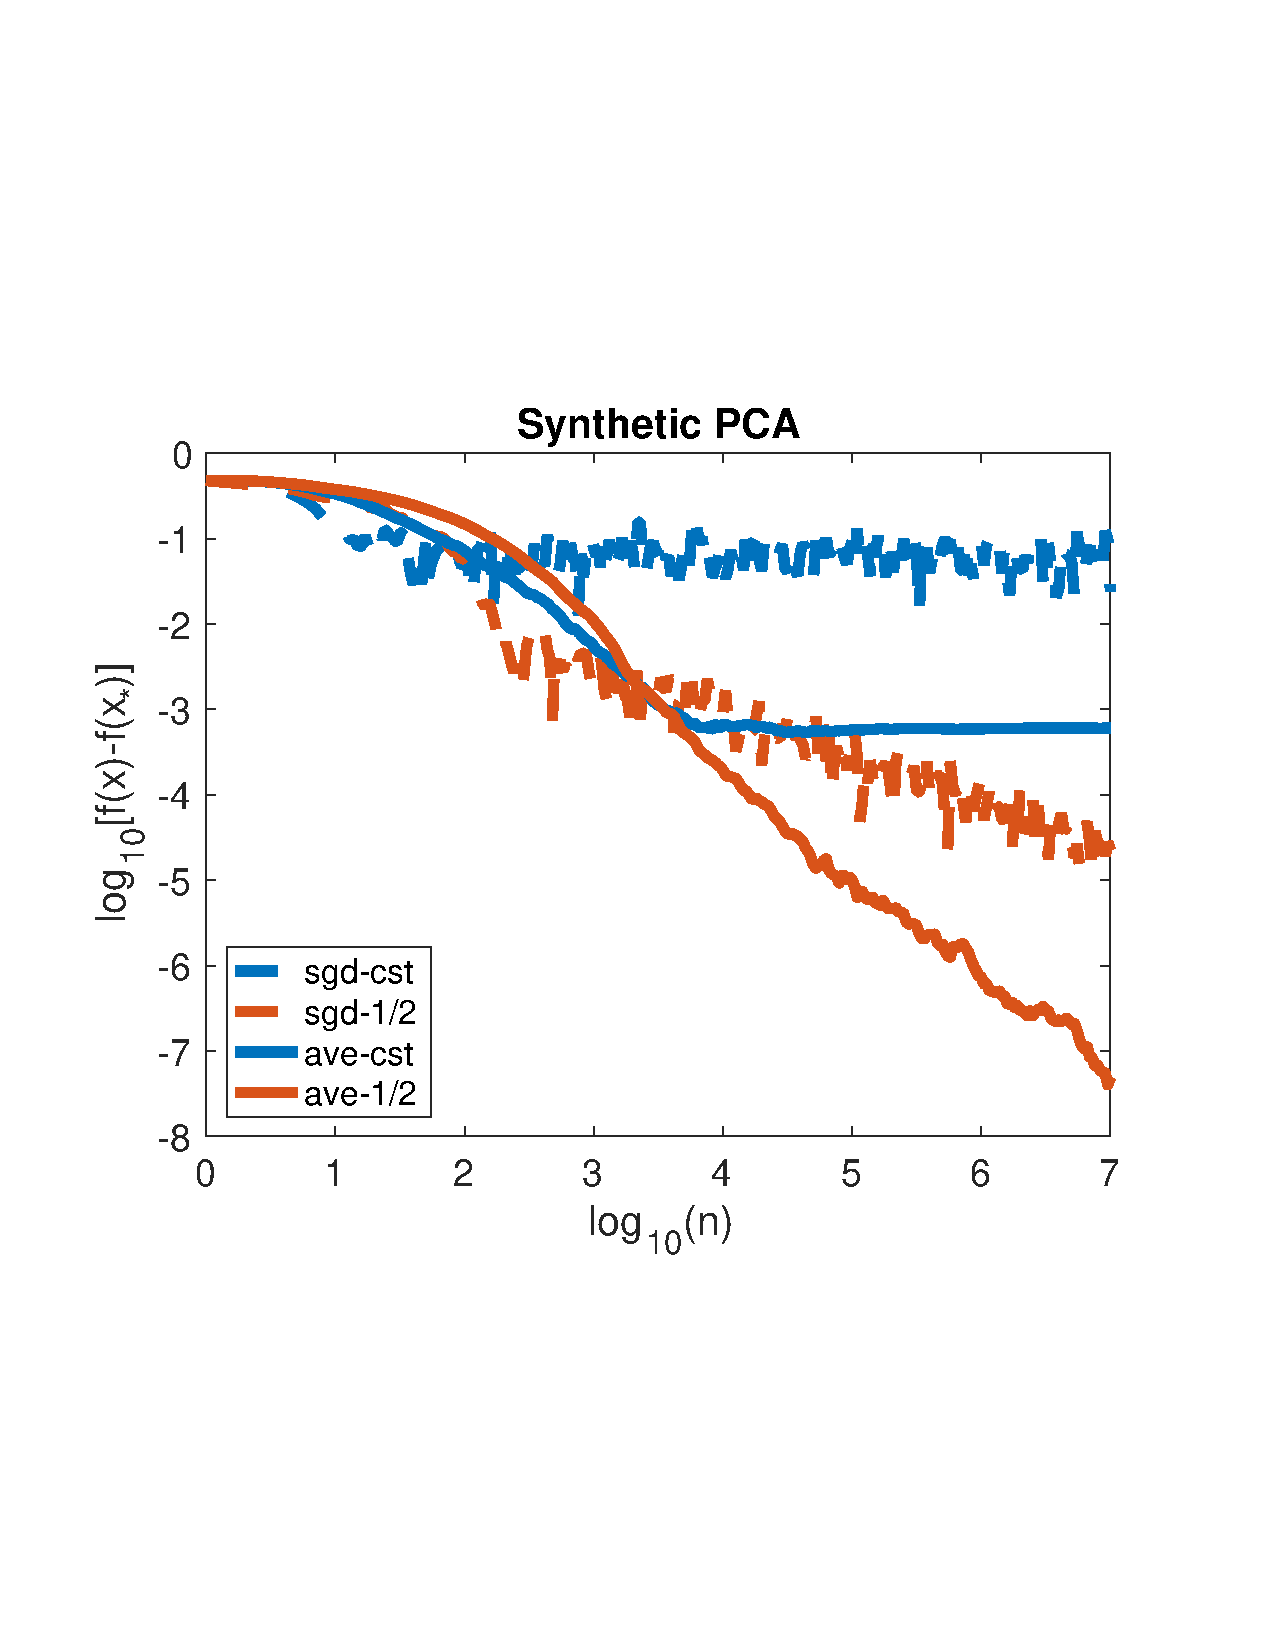
\includegraphics[width=0.8\linewidth]{Figs/counter2.pdf}
  \vspace{-3.0cm}
  \caption{Counterexample for the convergence of averaged SGD with constant step size.}
     \label{fig:counter}
\end{figure}
In this section we present an additional experiment which shows empirically that averaged SGD with constant step-size does not always converge for the streaming $k$-PCA problem. We consider $d=2$ and  a covariance matrice $H$ with random eigenvectors and two eigenvalues $\frac{1\pm1/\pi}{4}$. The noise distribution of the stream $\{h_n h_n^\top \}_{n\geq0}$ uses a more involved construction. Consider $\alpha_n\sim\mathcal N(-\pi/2,\pi^2/4)$ and $\beta_n\sim\mathcal N(\pi/4,\pi^2/16)$ and $\tau_n\sim \mathcal{B}(1/2)$. Then define $\theta_n$ as:
\[
\theta_n= \tau_n \alpha_n+(1-\tau_n)\beta_n,
\]
and the stream $h_n$ to be
\[
h_n= \Big[\frac{\cos(\theta_n)}{\sqrt{(1-1/\pi)/2}}, \frac{\sin(\theta_n)}{\sqrt{(1+1/\pi)/2}}\Big].
\]
\myfig{counter}, compares the performance of averaged SGD with constant step size $\gamma=1$ and the decreasing step size $\gamma_n=\frac{1}{\sqrt{n}}$. We see that with constant step size both SGD and averaged SGD do not converge to the true solution. SGD oscillates around the solution in ball of radius $\sim \gamma$ and averaged SGD does converge but not to the correct solution (although is still contained in a ball of radius $\sim 10^{-4}$ around the correct solution). On the other hand, SGD with decreasing step size behaves just as well as with a Gaussian data stream. SGD converges to the solution at the slow rate $O(1/\sqrt{n})$, while averaged SGD converges at the fast rate $O(1/{n})$.

This interesting example shows that constant step size averaged SGD does not converge to the correct solution in all situations. However, it remains a open problem to investigate the convergence properties of constant step size SGD in the Gaussian case.


\end{document}
